% Original License:
% CC BY-NC-SA 3.0 (http://creativecommons.org/licenses/by-nc-sa/3.0/)
%%%%%%%%%%%%%%%%%%%%%%%%%%%%%%%%%%%%%%%%%

\documentclass[11pt,fleqn]{book} 

\usepackage[top=3cm,bottom=3cm,left=3.2cm,right=3.2cm,headsep=10pt,letterpaper]{geometry}

\usepackage{xcolor}
\definecolor{ocre}{RGB}{52,177,201} 

\usepackage{avant} 
%\usepackage{times} % Use the Times font for headings
\usepackage{mathptmx} 
\usepackage{microtype} 
\usepackage[utf8]{inputenc}
\usepackage{mathrsfs}
\usepackage{graphicx}
\usepackage{caption}
\usepackage{subfigure}
\usepackage{wrapfig}
\usepackage{float}
\usepackage{braket}
\usepackage{multicol}
\usepackage{siunitx}
\usepackage{comment}



\usepackage[T1]{fontenc} 
%\usepackage[style=alphabetic,sorting=nyt,sortcites=true,autopunct=true,babel=hyphen,hyperref=true,abbreviate=false,backref=true,backend=biber]{biblatex}
%\addbibresource{ref-statistics.bib}
%\defbibheading{bibempty}{}


%%%%%%%%%%%%%%%%%%%%%%%%%%%%%%%%%%%%%%%%%
% This is based on the Legrand Orange Book
% Structural Definitions File
%
% The original template (the Legrand Orange Book Template) can be found here --> http://www.latextemplates.com/template/the-legrand-orange-book
%
% Original author of the Legrand Orange Book Template::
% Mathias Legrand (legrand.mathias@gmail.com) with modifications by:
% Vel (vel@latextemplates.com)
%
% Original License:
% CC BY-NC-SA 3.0 (http://creativecommons.org/licenses/by-nc-sa/3.0/)
%
%%%%%%%%%%%%%%%%%%%%%%%%%%%%%%%%%%%%%%%%%
%----------------------------------------------------------------------------------------
%	VARIOUS REQUIRED PACKAGES
%----------------------------------------------------------------------------------------

\usepackage{titlesec} % Allows customization of titles

\usepackage{graphicx} % Required for including pictures
\graphicspath{{Pictures/}} % Specifies the directory where pictures are stored

\usepackage{lipsum} % Inserts dummy text

\usepackage{tikz} % Required for drawing custom shapes

\usepackage[english]{babel} % English language/hyphenation

\usepackage{enumitem} % Customize lists
\setlist{nolistsep} % Reduce spacing between bullet points and numbered lists

\usepackage{booktabs} % Required for nicer horizontal rules in tables

\usepackage{eso-pic} % Required for specifying an image background in the title page

%----------------------------------------------------------------------------------------
%	MAIN TABLE OF CONTENTS
%----------------------------------------------------------------------------------------

\usepackage{titletoc} % Required for manipulating the table of contents

\contentsmargin{0cm} % Removes the default margin
% Chapter text styling
\titlecontents{chapter}[1.25cm] % Indentation
{\addvspace{15pt}\large\sffamily\bfseries} % Spacing and font options for chapters
{\color{ocre!60}\contentslabel[\Large\thecontentslabel]{1.25cm}\color{ocre}} % Chapter number
{}  
{\color{ocre!60}\normalsize\sffamily\bfseries\;\titlerule*[.5pc]{.}\;\thecontentspage} % Page number
% Section text styling
\titlecontents{section}[1.25cm] % Indentation
{\addvspace{5pt}\sffamily\bfseries} % Spacing and font options for sections
{\contentslabel[\thecontentslabel]{1.25cm}} % Section number
{}
{\sffamily\hfill\color{black}\thecontentspage} % Page number
[]
% Subsection text styling
\titlecontents{subsection}[1.25cm] % Indentation
{\addvspace{1pt}\sffamily\small} % Spacing and font options for subsections
{\contentslabel[\thecontentslabel]{1.25cm}} % Subsection number
{}
{\sffamily\;\titlerule*[.5pc]{.}\;\thecontentspage} % Page number
[] 

%----------------------------------------------------------------------------------------
%	MINI TABLE OF CONTENTS IN CHAPTER HEADS
%----------------------------------------------------------------------------------------

% Section text styling
\titlecontents{lsection}[0em] % Indendating
{\footnotesize\sffamily} % Font settings
{}
{}
{}

% Subsection text styling
\titlecontents{lsubsection}[.5em] % Indentation
{\normalfont\footnotesize\sffamily} % Font settings
{}
{}
{}
 
%----------------------------------------------------------------------------------------
%	PAGE HEADERS
%----------------------------------------------------------------------------------------

\usepackage{fancyhdr} % Required for header and footer configuration

\pagestyle{fancy}
\renewcommand{\chaptermark}[1]{\markboth{\sffamily\normalsize\bfseries\chaptername\ \thechapter.\ #1}{}} % Chapter text font settings
\renewcommand{\sectionmark}[1]{\markright{\sffamily\normalsize\thesection\hspace{5pt}#1}{}} % Section text font settings
\fancyhf{} \fancyhead[LE,RO]{\sffamily\normalsize\thepage} % Font setting for the page number in the header
\fancyhead[LO]{\rightmark} % Print the nearest section name on the left side of odd pages
\fancyhead[RE]{\leftmark} % Print the current chapter name on the right side of even pages
\renewcommand{\headrulewidth}{0.5pt} % Width of the rule under the header
\addtolength{\headheight}{2.5pt} % Increase the spacing around the header slightly
\renewcommand{\footrulewidth}{0pt} % Removes the rule in the footer
\fancypagestyle{plain}{\fancyhead{}\renewcommand{\headrulewidth}{0pt}} % Style for when a plain pagestyle is specified

% Removes the header from odd empty pages at the end of chapters
\makeatletter
\renewcommand{\cleardoublepage}{
\clearpage\ifodd\c@page\else
\hbox{}
\vspace*{\fill}
\thispagestyle{empty}
\newpage
\fi}

%----------------------------------------------------------------------------------------
%	THEOREM STYLES
%----------------------------------------------------------------------------------------

\usepackage{amsmath,amsfonts,amssymb,amsthm} % For math equations, theorems, symbols, etc

\newcommand{\intoo}[2]{\mathopen{]}#1\,;#2\mathclose{[}}
\newcommand{\ud}{\mathop{\mathrm{{}d}}\mathopen{}}
\newcommand{\intff}[2]{\mathopen{[}#1\,;#2\mathclose{]}}
\newtheorem{notation}{Notation}[chapter]

%%%%%%%%%%%%%%%%%%%%%%%%%%%%%%%%%%%%%%%%%%%%%%%%%%%%%%%%%%%%%%%%%%%%%%%%%%%
%%%%%%%%%%%%%%%%%%%% dedicated to boxed/framed environements %%%%%%%%%%%%%%
%%%%%%%%%%%%%%%%%%%%%%%%%%%%%%%%%%%%%%%%%%%%%%%%%%%%%%%%%%%%%%%%%%%%%%%%%%%
\newtheoremstyle{ocrenumbox}% % Theorem style name
{0pt}% Space above
{0pt}% Space below
{\normalfont}% % Body font
{}% Indent amount
{\small\bf\sffamily\color{ocre}}% % Theorem head font
{\;}% Punctuation after theorem head
{0.25em}% Space after theorem head
{\small\sffamily\color{ocre}\thmname{#1}\nobreakspace\thmnumber{\@ifnotempty{#1}{}\@upn{#2}}% Theorem text (e.g. Theorem 2.1)
\thmnote{\nobreakspace\the\thm@notefont\sffamily\bfseries\color{black}---\nobreakspace#3.}} % Optional theorem note
\renewcommand{\qedsymbol}{$\blacksquare$}% Optional qed square

\newtheoremstyle{blacknumex}% Theorem style name
{5pt}% Space above
{5pt}% Space below
{\normalfont}% Body font
{} % Indent amount
{\small\bf\sffamily}% Theorem head font
{\;}% Punctuation after theorem head
{0.25em}% Space after theorem head
{\small\sffamily{\tiny\ensuremath{\blacksquare}}\nobreakspace\thmname{#1}\nobreakspace\thmnumber{\@ifnotempty{#1}{}\@upn{#2}}% Theorem text (e.g. Theorem 2.1)
\thmnote{\nobreakspace\the\thm@notefont\sffamily\bfseries---\nobreakspace#3.}}% Optional theorem note

\newtheoremstyle{blacknumbox} % Theorem style name
{0pt}% Space above
{0pt}% Space below
{\normalfont}% Body font
{}% Indent amount
{\small\bf\sffamily}% Theorem head font
{\;}% Punctuation after theorem head
{0.25em}% Space after theorem head
{\small\sffamily\thmname{#1}\nobreakspace\thmnumber{\@ifnotempty{#1}{}\@upn{#2}}% Theorem text (e.g. Theorem 2.1)
\thmnote{\nobreakspace\the\thm@notefont\sffamily\bfseries---\nobreakspace#3.}}% Optional theorem note

%%%%%%%%%%%%%%%%%%%%%%%%%%%%%%%%%%%%%%%%%%%%%%%%%%%%%%%%%%%%%%%%%%%%%%%%%%%
%%%%%%%%%%%%% dedicated to non-boxed/non-framed environements %%%%%%%%%%%%%
%%%%%%%%%%%%%%%%%%%%%%%%%%%%%%%%%%%%%%%%%%%%%%%%%%%%%%%%%%%%%%%%%%%%%%%%%%%
\newtheoremstyle{ocrenum}% % Theorem style name
{5pt}% Space above
{5pt}% Space below
{\normalfont}% % Body font
{}% Indent amount
{\small\bf\sffamily\color{ocre}}% % Theorem head font
{\;}% Punctuation after theorem head
{0.25em}% Space after theorem head
{\small\sffamily\color{ocre}\thmname{#1}\nobreakspace\thmnumber{\@ifnotempty{#1}{}\@upn{#2}}% Theorem text (e.g. Theorem 2.1)
\thmnote{\nobreakspace\the\thm@notefont\sffamily\bfseries\color{black}---\nobreakspace#3.}} % Optional theorem note
\renewcommand{\qedsymbol}{$\blacksquare$}% Optional qed square
\makeatother

% Defines the theorem text style for each type of theorem to one of the three styles above
\newcounter{dummy} 
\numberwithin{dummy}{section}
\theoremstyle{ocrenumbox}
\newtheorem{theoremeT}[dummy]{Teorema}
\newtheorem{problem}{Problema}[chapter]
\newtheorem{exerciseT}{Ejercicio}[chapter]
\theoremstyle{blacknumex}
\newtheorem{exampleT}{Ejemplo}[chapter]
\theoremstyle{blacknumbox}
\newtheorem{vocabulary}{Vocabulario}[chapter]
\newtheorem{definitionT}{Definición}[section]
\newtheorem{corollaryT}[dummy]{Corollary}
\theoremstyle{ocrenum}
\newtheorem{proposition}[dummy]{Proposition}

%----------------------------------------------------------------------------------------
%	DEFINITION OF COLORED BOXES
%----------------------------------------------------------------------------------------

\RequirePackage[framemethod=default]{mdframed} % Required for creating the theorem, definition, exercise and corollary boxes

% Theorem box
\newmdenv[skipabove=7pt,
skipbelow=7pt,
backgroundcolor=black!5,
linecolor=ocre,
innerleftmargin=5pt,
innerrightmargin=5pt,
innertopmargin=5pt,
leftmargin=0cm,
rightmargin=0cm,
innerbottommargin=5pt]{tBox}

% Exercise box	  
\newmdenv[skipabove=7pt,
skipbelow=7pt,
rightline=false,
leftline=true,
topline=false,
bottomline=false,
backgroundcolor=ocre!10,
linecolor=ocre,
innerleftmargin=5pt,
innerrightmargin=5pt,
innertopmargin=5pt,
innerbottommargin=5pt,
leftmargin=0cm,
rightmargin=0cm,
linewidth=4pt]{eBox}	

% Definition box
\newmdenv[skipabove=7pt,
skipbelow=7pt,
rightline=false,
leftline=true,
topline=false,
bottomline=false,
linecolor=ocre,
innerleftmargin=5pt,
innerrightmargin=5pt,
innertopmargin=0pt,
leftmargin=0cm,
rightmargin=0cm,
linewidth=4pt,
innerbottommargin=0pt]{dBox}	

% Corollary box
\newmdenv[skipabove=7pt,
skipbelow=7pt,
rightline=false,
leftline=true,
topline=false,
bottomline=false,
linecolor=gray,
backgroundcolor=black!5,
innerleftmargin=5pt,
innerrightmargin=5pt,
innertopmargin=5pt,
leftmargin=0cm,
rightmargin=0cm,
linewidth=4pt,
innerbottommargin=5pt]{cBox}

% Creates an environment for each type of theorem and assigns it a theorem text style from the "Theorem Styles" section above and a colored box from above
\newenvironment{theorem}{\begin{tBox}\begin{theoremeT}}{\end{theoremeT}\end{tBox}}
\newenvironment{exercise}{\begin{eBox}\begin{exerciseT}}{\hfill{\color{ocre}\tiny\ensuremath{\blacksquare}}\end{exerciseT}\end{eBox}}				  
\newenvironment{definition}{\begin{dBox}\begin{definitionT}}{\end{definitionT}\end{dBox}}	
\newenvironment{example}{\begin{exampleT}}{\hfill{\tiny\ensuremath{\blacksquare}}\end{exampleT}}		
\newenvironment{corollary}{\begin{cBox}\begin{corollaryT}}{\end{corollaryT}\end{cBox}}	

%----------------------------------------------------------------------------------------
%	REMARK ENVIRONMENT
%----------------------------------------------------------------------------------------

\newenvironment{remark}{\par\vspace{10pt}\small % Vertical white space above the remark and smaller font size
\begin{list}{}{
\leftmargin=35pt % Indentation on the left
\rightmargin=25pt}\item\ignorespaces % Indentation on the right
\makebox[-2.5pt]{\begin{tikzpicture}[overlay]
\node[draw=ocre!60,line width=1pt,circle,fill=ocre!25,font=\sffamily\bfseries,inner sep=2pt,outer sep=0pt] at (-15pt,0pt){\textcolor{ocre}{R}};\end{tikzpicture}} % Orange R in a circle
\advance\baselineskip -1pt}{\end{list}\vskip5pt} % Tighter line spacing and white space after remark

%----------------------------------------------------------------------------------------
%	SECTION NUMBERING IN THE MARGIN
%----------------------------------------------------------------------------------------

\makeatletter
\renewcommand{\@seccntformat}[1]{\llap{\textcolor{ocre}{\csname the#1\endcsname}\hspace{1em}}}                    
\renewcommand{\section}{\@startsection{section}{1}{\z@}
{-4ex \@plus -1ex \@minus -.4ex}
{1ex \@plus.2ex }
{\normalfont\large\sffamily\bfseries}}
\renewcommand{\subsection}{\@startsection {subsection}{2}{\z@}
{-3ex \@plus -0.1ex \@minus -.4ex}
{0.5ex \@plus.2ex }
{\normalfont\sffamily\bfseries}}
\renewcommand{\subsubsection}{\@startsection {subsubsection}{3}{\z@}
{-2ex \@plus -0.1ex \@minus -.2ex}
{.2ex \@plus.2ex }
{\normalfont\small\sffamily\bfseries}}                        
\renewcommand\paragraph{\@startsection{paragraph}{4}{\z@}
{-2ex \@plus-.2ex \@minus .2ex}
{.1ex}
{\normalfont\small\sffamily\bfseries}}

%----------------------------------------------------------------------------------------
%	HYPERLINKS IN THE DOCUMENTS
%----------------------------------------------------------------------------------------

% For an unclear reason, the package should be loaded now and not later
\usepackage{hyperref}
\usepackage{hyperref}
\hypersetup{hidelinks,colorlinks=false,breaklinks=true,urlcolor= ocre,bookmarksopen=false,pdftitle={Title},pdfauthor={Author}}
%----------------------------------------------------------------------------------------
%	CHAPTER HEADINGS
%----------------------------------------------------------------------------------------

% The set-up below should be (sadly) manually adapted to the overall margin page septup controlled by the geometry package loaded in the main.tex document. It is possible to implement below the dimensions used in the goemetry package (top,bottom,left,right)... TO BE DONE

\newcommand{\thechapterimage}{}
\newcommand{\chapterimage}[1]{\renewcommand{\thechapterimage}{#1}}

% Numbered chapters with mini tableofcontents
\def\thechapter{\arabic{chapter}}
\def\@makechapterhead#1{
\thispagestyle{empty}
{\centering \normalfont\sffamily
\ifnum \c@secnumdepth >\m@ne
\if@mainmatter
\startcontents
\begin{tikzpicture}[remember picture,overlay]
\node at (current page.north west)
{\begin{tikzpicture}[remember picture,overlay]
\node[anchor=north west,inner sep=0pt] at (0,0) {\includegraphics[width=\paperwidth]{\thechapterimage}};
%%%%%%%%%%%%%%%%%%%%%%%%%%%%%%%%%%%%%%%%%%%%%%%%%%%%%%%%%%%%%%%%%%%%%%%%%%%%%%%%%%%%%
% Commenting the 3 lines below removes the small contents box in the chapter heading
%\fill[color=ocre!10!white,opacity=.6] (1cm,0) rectangle (8cm,-7cm);
%\node[anchor=north west] at (1.1cm,.35cm) {\parbox[t][8cm][t]{6.5cm}{\huge\bfseries\flushleft \printcontents{l}{1}{\setcounter{tocdepth}{2}}}};
\draw[anchor=west] (5cm,-9cm) node [rounded corners=20pt,fill=ocre!10!white,text opacity=1,draw=ocre,draw opacity=1,line width=1.5pt,fill opacity=.6,inner sep=12pt]{\huge\sffamily\bfseries\textcolor{black}{\thechapter. #1\strut\makebox[22cm]{}}};
%%%%%%%%%%%%%%%%%%%%%%%%%%%%%%%%%%%%%%%%%%%%%%%%%%%%%%%%%%%%%%%%%%%%%%%%%%%%%%%%%%%%%
\end{tikzpicture}};
\end{tikzpicture}}
\par\vspace*{230\p@}
\fi
\fi}

% Unnumbered chapters without mini tableofcontents (could be added though) 
\def\@makeschapterhead#1{
\thispagestyle{empty}
{\centering \normalfont\sffamily
\ifnum \c@secnumdepth >\m@ne
\if@mainmatter
\begin{tikzpicture}[remember picture,overlay]
\node at (current page.north west)
{\begin{tikzpicture}[remember picture,overlay]
\node[anchor=north west,inner sep=0pt] at (0,0) {\includegraphics[width=\paperwidth]{\thechapterimage}};
\draw[anchor=west] (5cm,-9cm) node [rounded corners=20pt,fill=ocre!10!white,fill opacity=.6,inner sep=12pt,text opacity=1,draw=ocre,draw opacity=1,line width=1.5pt]{\huge\sffamily\bfseries\textcolor{black}{#1\strut\makebox[22cm]{}}};
\end{tikzpicture}};
\end{tikzpicture}}
\par\vspace*{230\p@}
\fi
\fi
}
\makeatother
\addto\captionsenglish{\renewcommand{\figurename}{Fig.}}

\begin{document}
\title{FÍSICA ESTADÍSTICA}
%-------------------------------------------------
\begingroup
\thispagestyle{empty}
\AddToShipoutPicture*{\put(-580,0){\includegraphics[scale=0.1855]{stars}}}
\centering
\vspace*{5cm}
\par\normalfont\fontsize{35}{35}\sffamily\selectfont
\textbf{Física Estadística}\\
{\LARGE Notas de clase}\par
\vspace*{1cm}
%{\Huge Carlos José Páez Gonzalez}\par 
\endgroup
%--------------------------------------------------
\newpage
~\vfill
\thispagestyle{empty}

%\noindent Copyright \copyright\ 2014 Andrea Hidalgo\\ % Copyright notice
\noindent \textsc{Universidad Industrial de Santander \textbf{(UIS)} \\
Física Computacional en Materia Condensada  \textbf{(FICOMACO)}}\\
\url{http://www.uis.edu.co}\\

\noindent Profesor\\
Carlos José Páez Gonzalez\\
carlos.paez@uis.edu.co\\
\url{https://orcid.org/0000-0003-4037-064X}\\

\noindent Estudiante\\
Juan Alejandro Pinto Castro\\
alejopintirris@gmail.com\\
\url{https://orcid.org/0000-0002-0937-4848}\\

\noindent The original template (the Legrand Orange Book Template) can be found here:\\
\noindent \textsc{\url{http://www.latextemplates.com/template/the-legrand-orange-book}}\\ % URL

\noindent  This is based on the Legrand Orange Book. Original author of the Legrand Orange Book Template: Mathias Legrand (legrand.mathias@gmail.com) with modifications by: Vel (vel@latextemplates.com)
Original License: CC BY-NC-SA 3.0 (\url{http://creativecommons.org/licenses/by-nc-sa/3.0/}).\\ % License information

\noindent \textit{Primera Edición, Mayo 2020} % Printing/edition date
%--------------------------------------------------------------
\newpage
~\vfill
\thispagestyle{empty}
\noindent \begin{flushright}
\emph{"Soy consciente de ser sólo una persona que lucha débilmente contra la corriente del tiempo. Sin embargo, todavía me queda poder contribuir de tal manera que, cuando la teoría de los gases sea de nuevo reavivada, no tarde demasiado en ser redescubierta.“}\\
\vspace{3mm}
\textbf{- Ludwig Boltzmann}
\end{flushright}

%http://www.frasesypensamientos.com.ar/autor/irving-langmuir.html
%---------------------------------------------------

\chapterimage{plasma_light_line_abstraction.jpg} % Table of contents heading image

\pagestyle{empty} % No headers
\renewcommand\contentsname{Contenido}
\tableofcontents % Print the table of contents itself

%\cleardoublepage % Forces the first chapter to start on an odd page so it's on the right

\pagestyle{fancy} % Print headers again

%----------------------------------------------------------------------------------------
%	CHAPTER 1
%----------------------------------------------------------------------------------------

\chapterimage{plasma_hand.jpg} % Chapter heading image
\renewcommand{\chaptername}{}
\chapter{Teoría cinética de los gases}

\begin{quote}
\emph{"Conseguimos obtener así la fórmula estadística para conocer aproximadamente la posición de un electrón en un instante determinado. Pero, personalmente, no creo que dios juegue a los dados."}
\begin{flushright}
\textbf{-Albert Einstein}
\end{flushright}
\headrule
\end{quote}

\section{Introducción y Algo de Historia}

¿Como podemos describir las propiedades físicas de sistemas macroscópicos? Pregunta que se responde con la estadística y la termodinámica. Un sistema macroscópico es un sistema con un número muy grande de partículas, una parte de ese sistema es fenomenológico (\textbf{termodinámica}) y otra parte es probabilístico (\textbf{estadística}); cuando necesitamos entender el sistema microscópicamente, se usa la estadística.

\begin{figure}[H]
    \centering
    \subfigure[]{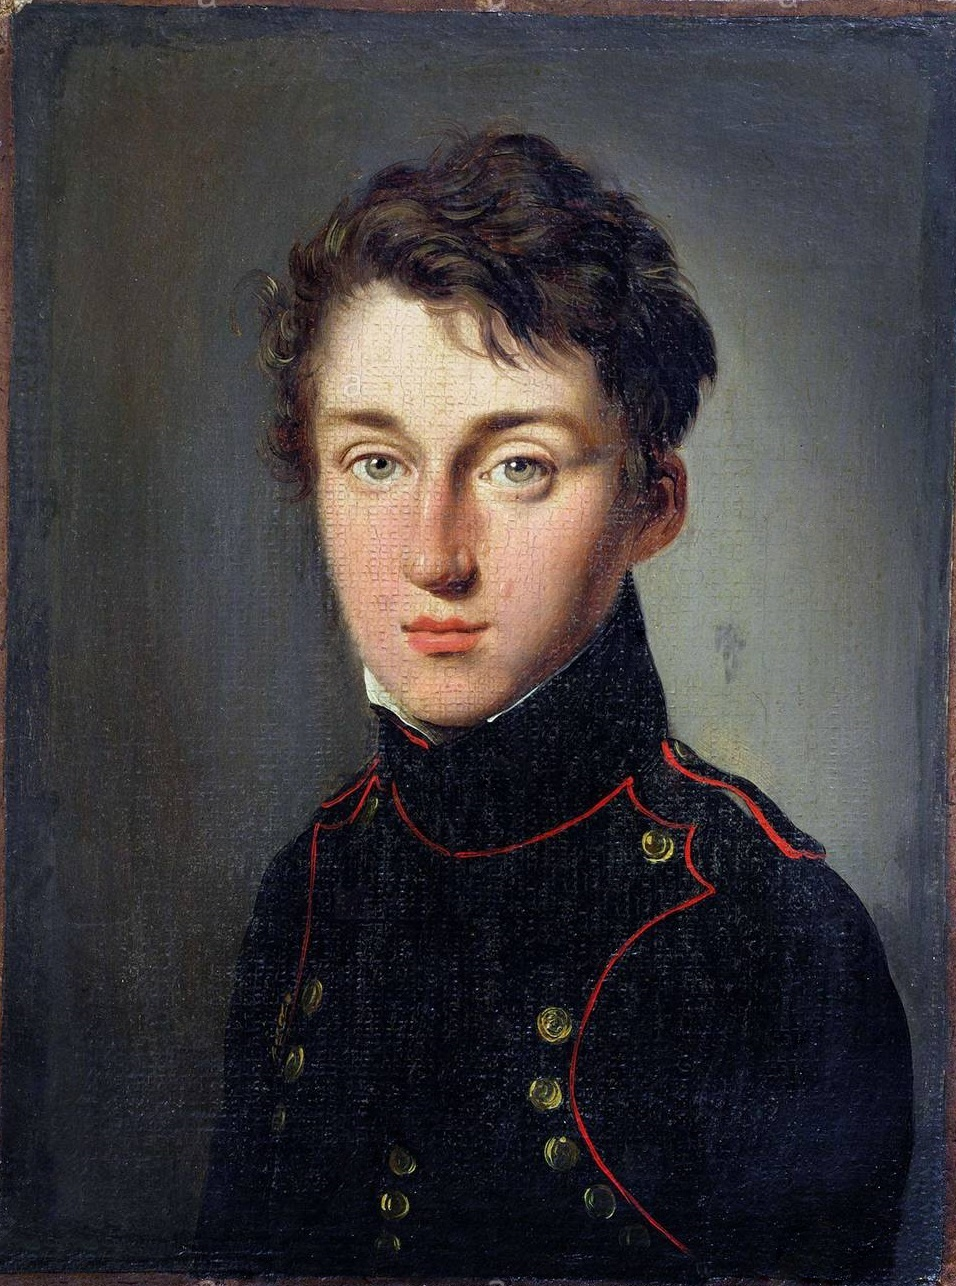
\includegraphics[width=0.207\textwidth]{zSadi_Carnot.jpeg}}
    \subfigure[]{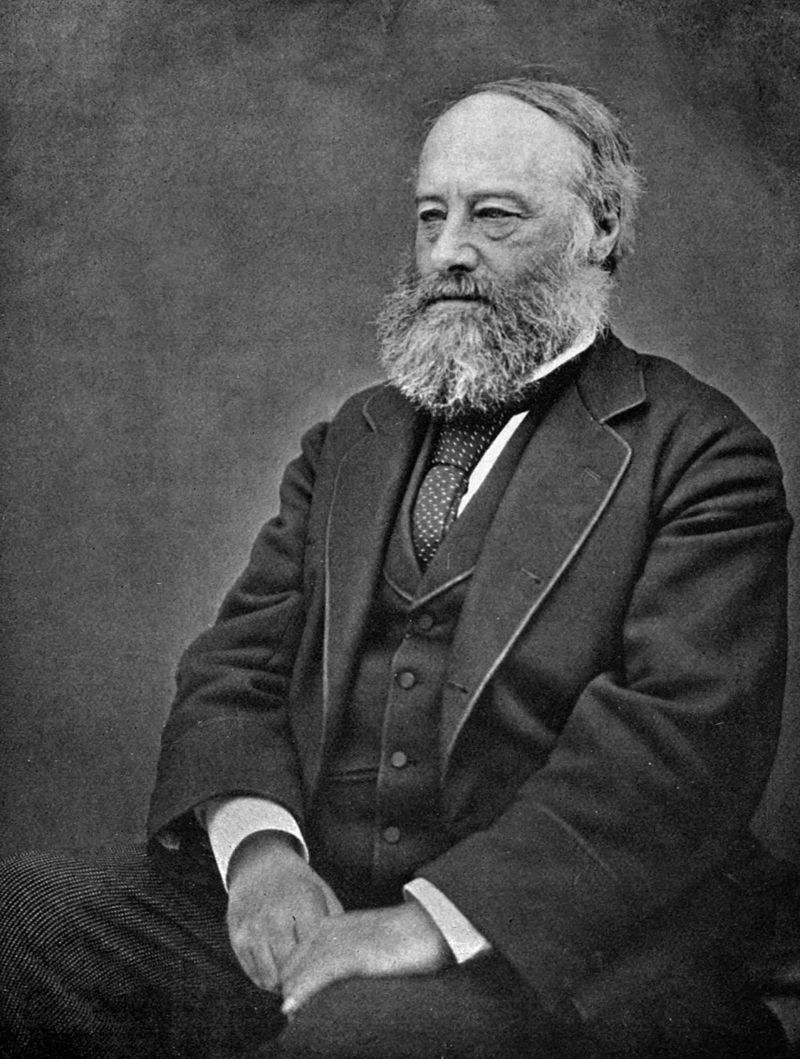
\includegraphics[width=0.21\textwidth]{zjoule.jpg}}
    \subfigure[]{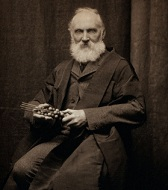
\includegraphics[width=0.246\textwidth]{zkelvin.jpg}}
    \subfigure[]{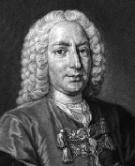
\includegraphics[width=0.227\textwidth]{zandercelsius1_62.jpg}}
    \caption{(a) Nicolas Carnot, (b) James Joule, (c) William Thomson (Baron Kelivn) y (d) Anders Celsius}
\end{figure}

La \textbf{termodinámica} nace entre el siglo \textsc{xix} y \textsc{xx} con autores que aportaron un poco de conocimiento, como Carnot (2 ley), Joule (1 ley), Kelvin, Celsius, los cuales describieron sistemas macroscópicos. La termodinámica surge a partir de resultados experimentales, es una consecuencia de tener limitaciones en las mediciones. Si medimos el tiempo en segundos, comparado con tiempos microscópicos como la velocidad a la que gira el electrón alrededor de su núcleo, es un tiempo muy grande, cuando medimos, el sistema ya esta en equilibrio; el equilibrio termodinámico puede ser descrito por unas variables, como presión, temperatura, volumen. Un sistema en equilibrio termodinámico tiene tres tipos de equilibrio:

\begin{itemize}
    \item \textbf{Térmico:} intercambio de energía (temperatura)
    \item \textbf{Mecánico:}intercambio de volumen (presión)
    \item \textbf{Difusivo:} intercambio de partículas (potencial químico)
\end{itemize}
     
El sistema tiene que estar intercambiando algo, siempre va a buscar el equilibrio (2 ley), y cuando llega al equilibrio, llega de las tres formas, no una ni dos. El sistema tiene un tiempo de relajación para llegar al equilibrio, ahí es donde surge el  intento de la termodinámica por definir que es la temperatura, ligada con el calor, que se refiere a los procesos de intercambio de energía, ligada con sistemas microscópicos.

\begin{figure}[H]
    \centering
    \subfigure[]{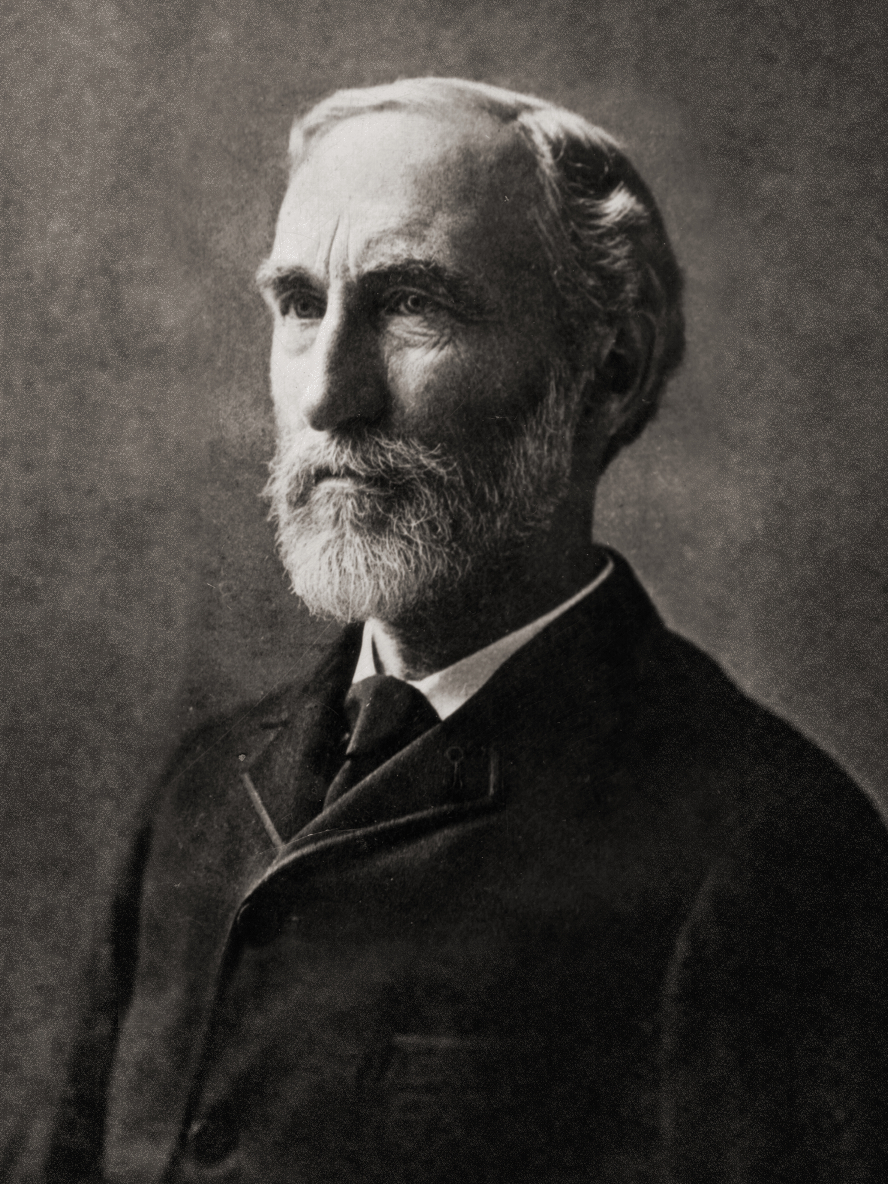
\includegraphics[width=0.213\textwidth]{zgibbs.jpg}}
    \subfigure[]{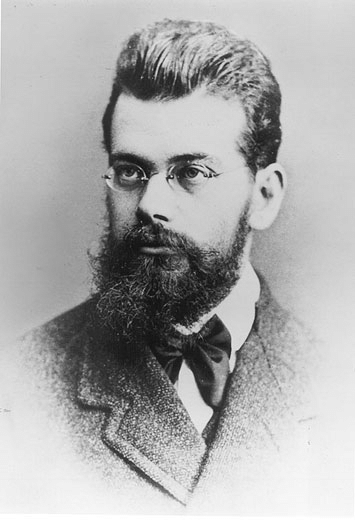
\includegraphics[width=0.194\textwidth]{zboltzmann.png}}
    \subfigure[]{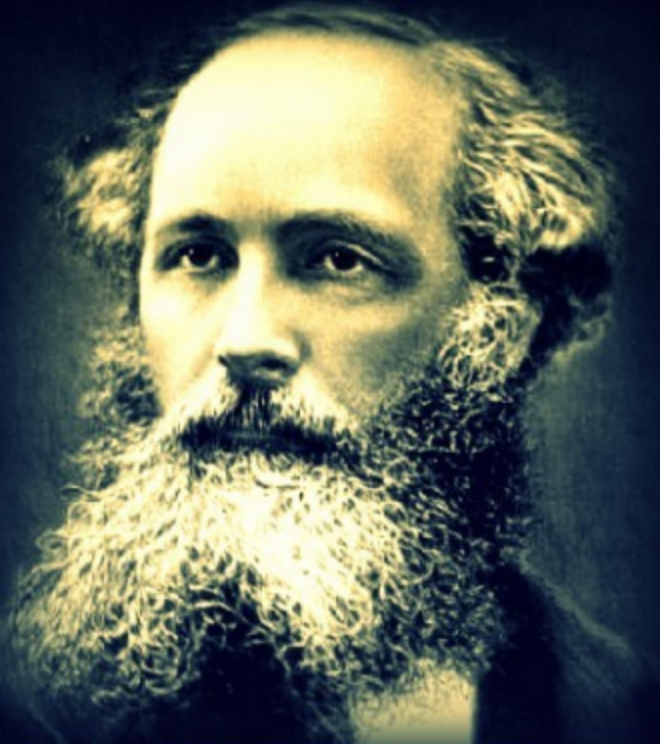
\includegraphics[width=0.252\textwidth]{zmaxwell.jpg}}
    \subfigure[]{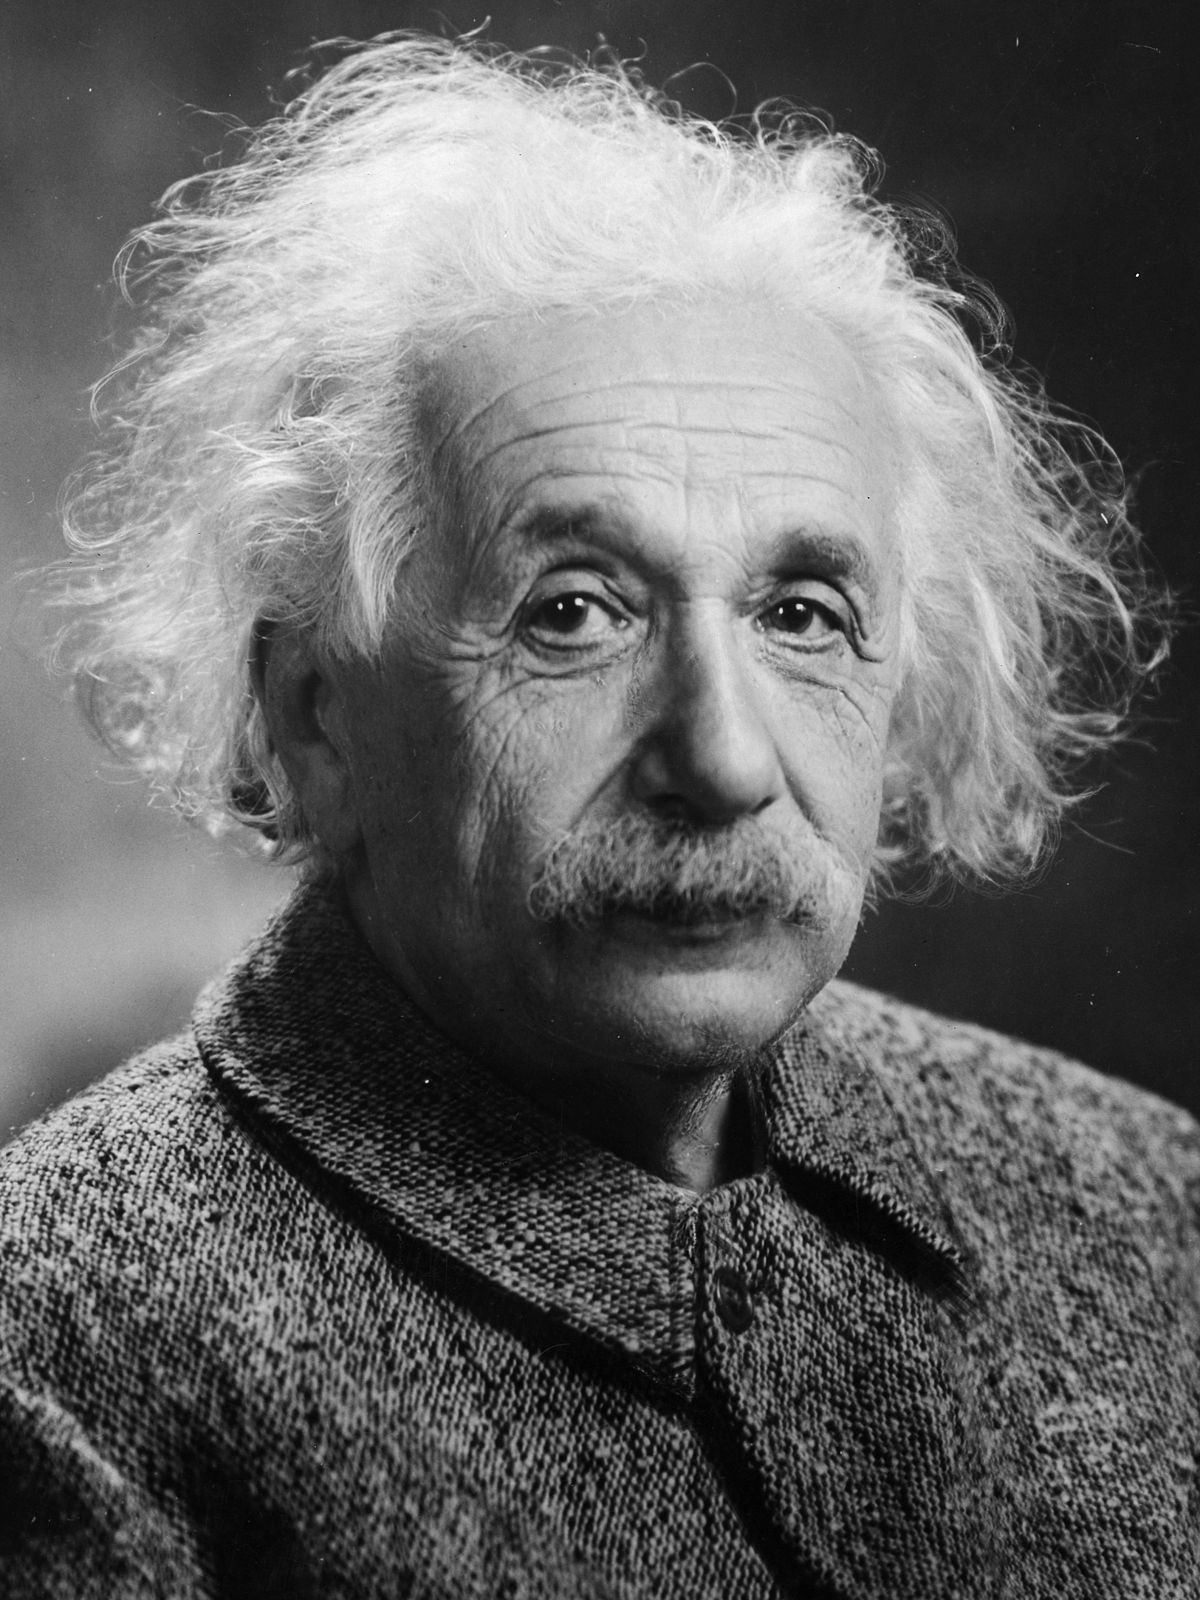
\includegraphics[width=0.214\textwidth]{zAlbert_Einstein_Head.jpg}}
    \caption{(a) Josiah Gibbs, (b) Ludwig Boltzmann, (c) James Maxwell y (d) Albert Einstein }
\end{figure}

La \textbf{estadística} inició entre el siglo \textsc{xix} y \textsc{xx}, aportaron grandes ideas como Gibbs, Boltzmann, Maxwell, Einstein. Gibbs definió un ensamble, son muchos sistemas microscópico que se comportan como un sistema macroscópico, lo que medimos es un promedio de lo que le pasa a los sistemas microscópicos. Boltzmann postuló \textit{la hipótesis ergódica} (diferente a la teoría ergódica), dice que si tenemos ensambles y esperamos un tiempo diferente, todos van a ser igualmente probables. También definió \textit{la ecuación maestra} o ecuación de transporte, un sistema demora cierto tiempo en llegar al equilibrio. También habló sobre el \textit{teorema H}, intentó describir las leyes de la termodinámica a partir de la probabilidad, postuló la \textit{teoría cinética de los gases}, una teoría que implicaba la irreversibilidad temporal, lo que lo llevó a suicidarse por ser incomprendido. La estadística tiene dos objetivos claros:

\begin{itemize}
    \item Intenta deducir las leyes de la termodinámica, no ha sido posible hasta ahora.
    \item Calcular las propiedades físicas considerando que las coordenadas microscópicas de los observables pueden ser tratadas probabilísticamente.
\end{itemize}

\section{Modelo mecánico microscópico}

Volviendo a la temperatura, es lo que se mide en el termómetro, se relaciona con las características físicas del sistema. Celsius habló primero de los termómetros, las propiedades que podemos medir del mercurio en una columna están relacionadas con la temperatura la cual modifica otras propiedades; midió el volumen de la columna cerca del hielo y observó que tiende a disminuir su volumen, luego colocó el termómetro sobre agua evaporándose y definió su escala. Un gas cuántico es un gas muy denso, las partículas interactúan entre sí y esas interacciones se describen cuánticamente. Se creó un termómetro basado en gas, pero con una baja concentración de partículas, que se comportan de forma lineal. La escala Kelvin surgió de este termómetro.

La ecuación de estado para un gas ideal es:
\begin{equation}
    PV=nRT
    \label{Eq-ideal-gas}
\end{equation}

Donde la temperatura se mide en Kelvin $[K]$, el número de moles del gas $n=\frac{N}{n_{A}}$, donde $N_{A}$ es la constante de Avogadro, $R=8,31 [\frac{J}{molK}]$, entonces podemos reescribir la ecuación \ref{Eq-ideal-gas} como:

\begin{equation}
    Pv=N\left(\frac{R}{N_{A}}\right)T=Nk_{b}T
\end{equation}

Donde $k_{b}$ representa la constante de Boltzmann $1.38 [\frac{J}{K}]$, esta constante dice que existe una relación entre energía y temperatura, también se puede ver como una conversión entre estas dos variables. 

\begin{figure}[H]
    \begin{minipage}[c]{0.6\linewidth}
    \hspace{5mm} Daniel Bernoulli establece el modelo mecánico de un gas ideal, supone un pistón de longitud $l$ y área $A$ que contiene un gas ideal, las partículas que componen el gas no interactúan, solo tienen energía y chocan elásticamente con las paredes, tienen velocidad y masa. Estas aplican una fuerza sobre la pared que depende del cambio del momento en un tiempo pequeño de interacción con la pared, entonces ¿Qué fuerza ejerce la partícula sobre la pared?, en un tiempo t:
    \end{minipage}\hspace{1cm}
    \begin{minipage}[c]{0.5\linewidth}
    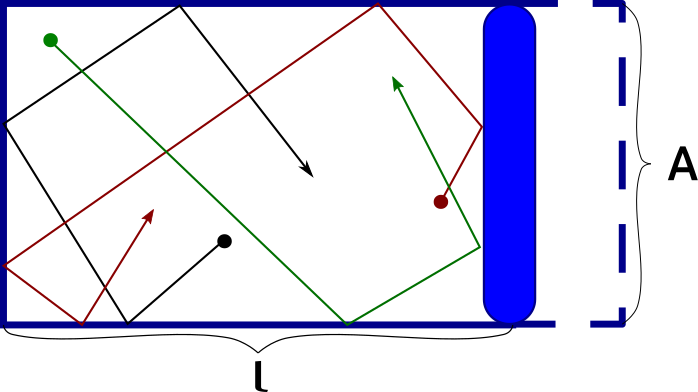
\includegraphics[width=0.7\textwidth]{text12388.png}
    \end{minipage}
\end{figure}
\vspace{-9mm} 

\begin{equation}
    F \Delta t =2m\Bar{v}_{x}
    \label{Eq. 1.3}
\end{equation}

Las partículas vuelven a chocar con la pared pero con velocidad negativa, $\Delta t = \frac{2l}{\bar{v}_{x}}$, reemplazando en la ecuación \ref{Eq. 1.3}, la fuerza queda como:

\begin{equation}
   Fl=m\bar{v}_{x}^{2}
   \label{Eq. 1.4}
\end{equation}

La ecuación \ref{Eq. 1.4} es la fuerza promedio. La presión promedio es $P=\frac{F}{A}$, entonces:

\begin{equation}
PV=m\bar{v}_{x}^{2}
\label{Eq. 1.5}
\end{equation}

Suponemos que la velocidad en todas las direcciones es la misma, $v_{x}=v_{y}=v_{z}$, entonces $\bar{v}^{2}=3v_{x}^{2}$; reemplazando esta igualdad en la ecuación \ref{Eq. 1.5}, y definiendo la energía cinética de la partículas como $K=\frac{1}{2}m\bar{v}^{2}$, tenemos:

\begin{equation}
    PV=\frac{2}{3}N\frac{m\bar{v}^{2}}{3}=Nk_{b}T
    \label{Eq. 1.6}
\end{equation}

Según la anterior ecuación, la energía cinética es:

\begin{equation}
    K_{t}=\frac{3}{2}k_{B}T
    \label{Eq. 1.7}
\end{equation}

La energía cinética es una  cantidad microscópica, mientras que la temperatura es una cantidad macroscópica, es decir la interpretación física de la ecuación \ref{Eq. 1.7} es que la temperatura es la energía cinética de las partículas.

\subsection{Energía}

La temperatura $T$ es una característica macroscópica que determina una característica microscópica $K_{t}$ como se menciona en la ecuación \ref{Eq. 1.7}. Si extrapolamos este resultado a los conceptos de la mecánica clásica, vemos que la energía cinética,

\begin{equation}
    K_{t}=\frac{1}{2}m\left(\bar{v}_{x}^{2}+\bar{v}_{y}^{2}+\bar{v}_{z}^{2}\right)=\frac{3}{2}k_{B}T
    \label{Eq. 1.8}
\end{equation}

representa una ligadura holónoma del sistema, es decir no contribuye a reducir los grados de libertad. Cuando construimos la energía, el número de grados de libertad que tenemos depende de la cantidad de términos que le sumamos a la energía, en el caso de la ecuación \ref{Eq. 1.8}, el sistema tiene 3 términos que corresponden a 3 grados de libertad.

\begin{theorem}[Equipartición]
Por cada grado de libertad cuadrático, a la energía se adiciona $\frac{1}{2}k_{B}T$.

\begin{example}
Una molécula diatómica (Fig. \ref{Fig. 1.4}(a)) tiene un hamiltoniano de la forma:

\begin{align*}
      H=&\frac{M}{2}\left(p_{x}^{2}+p_{y}^{2}+p_{z}^{2}\right) && \text{Traslacional con 3 grados de libertad}\\
      &+\frac{p_{\theta}^{2}}{2mr^{2}}+\frac{p_{\phi}^{2}}{2mr^{2}sin(\theta)} && \text{Rotacional con 2 grados de libertad}\\
      &+\frac{p_{R}^{2}}{2mr}+\frac{K_{e}R^{2}}{2} && \text{Vibracional con 2 grados de libertad}
\end{align*}

\noindent La molécula diatómica puede girar con respecto al eje $x$ y $y$ pero por simetría no puede girar con el eje $z$, la traslación con respecto al centro de masa, por cada término, se agrega $\frac{1}{2}k_{B}T$, si no hay un término cuadrático no se agrega, el cuadrático es la energía térmica del sistema, en el caso de la molécula diatómica viene siendo:

\begin{equation*}
    \braket{H}\quad=\quad\frac{3}{2}k_{B}T+\frac{2}{2}k_{B}T+\frac{2}{2}k_{B}T\quad=\quad\frac{7}{2}k_{B}T
\end{equation*}
\end{example}
\end{theorem}

De una forma más general, podemos escribir la energía térmica como:

\begin{equation}
    U_{ter}=Nf\frac{k_{B}T}{2}
    \label{Eq. 1.9}
\end{equation}

Donde $f$ es el número de grados de libertad activos en el sistema. Si la molécula esta formada de diferentes especies de átomos, se debe distinguir la energía de cada átomo. Así pues, se suma un término de energía que podría ser la interacción de los diferentes tipos de átomos que conforman la molécula.

\begin{equation*}
    U=U_{ter}+U_{otro}
\end{equation*}

\begin{figure}[H]
    \begin{minipage}[c]{0.6\linewidth}
    \hspace{5mm} La energía térmica está en términos de $k_{B}T$, si se tiene una temperatura de $300[K]$ en un sistema con 2 grados de libertad, la energía térmica sería alrededor de $\frac{1}{40}[eV]$. Si la energía de ionización que se necesita para expulsar un electrón de la  orbita nuclear en el estado base del átomo de hidrógeno (Fig. \ref{Fig. 1.3}) es de $E_{ion}\approx13.6 [eV]$, y si quisiera ionizar ese átomo térmicamente voy a necesitar una temperatura de 400 veces la temperatura inicial $T\approx544\cdot300\approx163200[K]$. Térmicamente no puedo separar el electrón del núcleo, necesitaría una temperatura demasiado alta. 
    \end{minipage}\hspace{7mm}
    \begin{minipage}[c]{0.5\linewidth}
    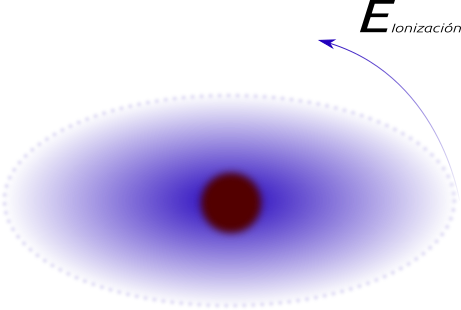
\includegraphics[width=0.6\textwidth]{electron.png}
    \caption{Electrón orbitando\\ sobre un plano en el átomo de H}
    \label{Fig. 1.3}
    \end{minipage}
\end{figure}
\vspace{-5mm} 

En  el caso de las moléculas, los grados de libertad de la molécula diatómica se activan a medida que se aumenta la temperatura, y por ende aumenta su energía. Los primeros estados en ser activados son traslacionales, luego rotacionales, por último vibracionales, como se muestra en la figura \ref{Fig. 1.4}(b). Con una energía alrededor de $300 [K]$, alcanzamos a activas los modos traslacionales y algunos rotacionales, los vibracionales existen pero es difícil activarlos, se encuentran congelados. La energía térmica del sistema va a ser el número de partículas que tengo con tres traslacionales y dos rotacionales. la mayoría de los resultados estudiados se van a tener en cuenta los traslacionales y rotacionales, por esta razón es común ver resultados con $\frac{5}{2}$, ejemplo $U_{ter}=N\frac{5}{2}k_{B}T$. 

\begin{figure}[H]
    \centering
    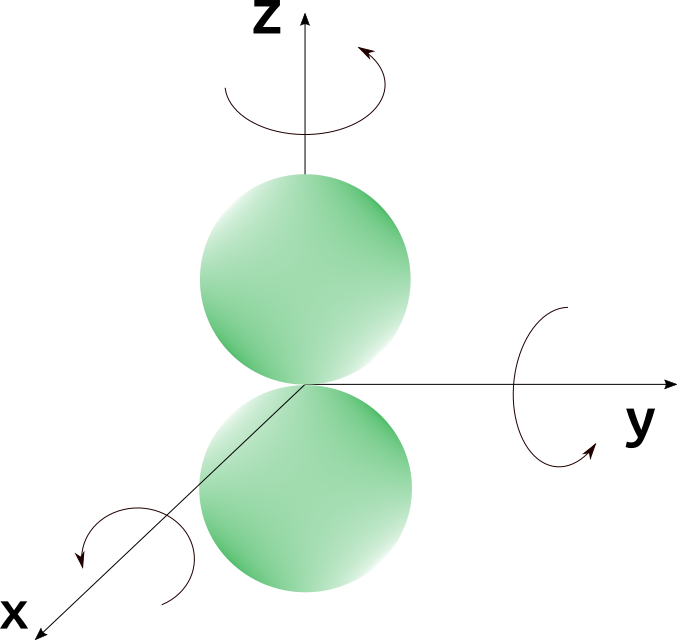
\includegraphics[width=0.4\textwidth]{molecule-di.png}\hspace{2cm}
    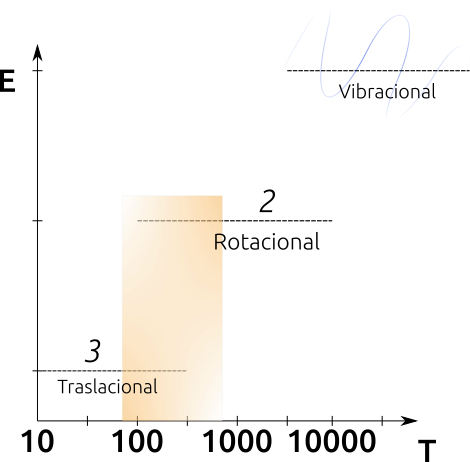
\includegraphics[width=0.45\textwidth]{evst.png}
    \caption{(a) Molécula diatómica. (b) Gráfica de capacidad calorífica a volumen constante ($C_{v}$) en función de la temperatura.}
    \label{Fig. 1.4}
\end{figure} 

El rompimiento de enlaces entre moléculas están vinculados con otro tipo de interacción, en las transiciones de fase no se rompen los átomos de la molécula, solo los enlaces entre las moléculas. Hablamos que en la energía térmica aportan $\frac{1}{2}k_{B}T$ solo a los grados de libertad con expresión cuadrático, los demás términos no dependen de la temperatura.

\section{Calor y trabajo}

En termodinámica definimos que el calor y el trabajo es un flujo de energía, en un sistema podemos ingresar energía de dos maneras: calor y trabajo. El calor es un flujo de energía que pasa de forma espontánea y es producido por la diferencia de temperatura. Ese calor que entra al sistema, consideramos que es mayor que cero, los demás tipos de flujo de energía que no es calor, lo consideramos como trabajo,que va a ser positivo si entra al sistema. la energía interna del sistema va a cambiar $\Delta U$ si estoy introduciendo $Q$ y $W$, el cambio en la energía interna es:

\begin{equation}
    \Delta U=Q+W \quad\longrightarrow\quad\mathrm{d}U=\mathrm{d_{i}}Q+\mathrm{d_{i}}W
    \label{Eq. 1.10}
\end{equation}

Conocida como la primera ley de la termodinámica, si el cambio es infinitesimal seguimos teniendo calor y trabajo, ni el calor ni el trabajo son cantidades variacionales.

\subsection{Mecanismos de transferencia}

Como transferimos calor o trabajo al sistema, los mecanismos de transferencia son: 

\begin{itemize}
    \item Conducción: se tiene contacto microscópico, hay choque de moléculas o contacto entre ellas.
    \item  Convección: exige un movimiento global del sistema. Al aumentar la temperatura disminuye su densidad, como están bajo campo gravitatorio todas las moléculas calentadas van a subir.
    \item  Radiación: relacionada con la radiación electromagnética. 
\end{itemize}

\begin{example}
cuando calentamos agua en microondas, el mecanismo de transferencia corresponde a trabajo a través de la radiación mas no motivado por una diferencia de temperatura. Cuando nos frotamos las manos, se realiza trabajo porque no hay diferencia de temperaturas. 
\end{example}

\subsection{Tipos de trabajo}

Existen muchos tipos de trabajo, pero nos enfocaremos en el trabajo de compresión que es la fuerza aplicada al sistema que produce un desplazamiento en el punto de aplicación de la fuerza o sobre el centro de masa dándole energía al sistema. Por el momento vamos a definir el desplazamiento en el punto donde se coloca la fuerza. En los demás trabajos no nos enfocaremos.

\begin{equation}
    W=W_{comp}+W_{otros}
    \label{Eq. 1.11}
\end{equation}

El trabajo de compresión lo definimos como:
\begin{equation}
    W_{comp}=\Vec{F}\cdot\mathrm{d}\Vec{r}\quad>\quad0
    \label{Eq. 1.12}
\end{equation}

El sistema debe llegar al equilibrio para relacionar variables como $PTV$, etc., el proceso es cuasiestático, se le da tiempo al sistema para que se acomode, este tiempo debe ser menor a la velocidad del sonido perturbación mecánica de sistema, que se transfiere en el sistema. Le doy tiempo al sistema de que se reacomode y llegue a los tres equilibrios: térmico, mecánico y difusivo. La presión debe ser homogénea, el requisito de compresión es que debe ser un proceso estático. Ese trabajo de compresión se puede definir través de la presión. como $P=\frac{F}{A}$, esta se reemplaza en la ecuación \ref{Eq. 1.12}: 

\begin{equation*}
    W_{comp}=PA\mathrm{d}x=-P\mathrm{d}V\quad>\quad0
\end{equation*}

Por la condición que se impuso sobre el trabajo positivo entrando al sistema, el menos surge debido a que el volúmen final va a ser menor que el inicial. La presión va a ser constante pero diferente para cada volumen, entonces lo puedo considerar como:

\begin{equation}
    W_{comp}=-\int_{V_{i}}^{V_{f}}P(V)\mathrm{d}V
    \label{Eq. 1.13}
\end{equation}

\section{Proceso cuasiestático}

Procesos cuasiestáticos pueden ser variados, pero nos enfocaremos en los procesos de dos maneras: isotérmico y adiabático, se realiza un poco mas rápida el proceso isotérmico que el adiabático $v_{i}<v_{a}$.

\subsection{Proceso isotérmico}

En un proceso isotérmico la temperatura es constante, entonces $\Delta T=0$ no cambia la temperatura, es decir sale calor pero esta entrando otro tipo de energía por movimiento, esto implica que cuando hago un proceso isotérmico, al comprimir el sistema le doy tiempo suficiente al sistema para que intercambie energía con el medio, la temperatura exterior va a ser igual a la temperatura interior. Un ejemplo de este proceso se observa en la figura \ref{Fig. 1.5}(a).

\begin{figure}[H]
    \centering
    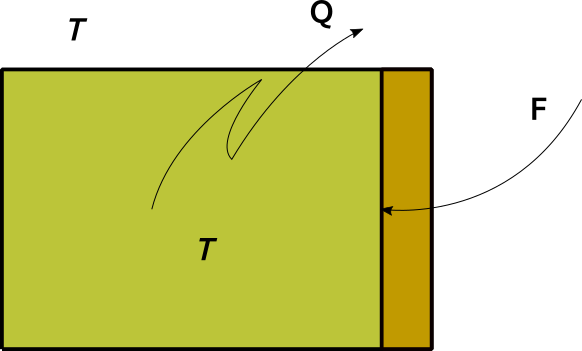
\includegraphics[width=0.55\textwidth]{isotermabox.png}\hspace{5mm}
    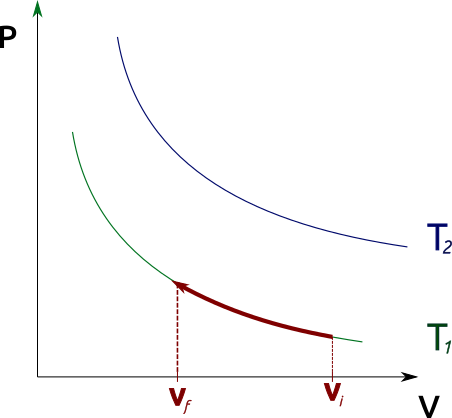
\includegraphics[width=0.35\textwidth]{isoterma.png}
    \caption{(a) Trabajo de compresión para mantener $T=cte$. (b) Gráfica de un proceso isotérmico.}
    \label{Fig. 1.5}
\end{figure} 

Para el gas ideal, lo que obtenemos en el diagrama $PV$ de la figura \ref{Fig. 1.5}(b) es que cuando se hace el proceso de forma isotérmica, me muevo de un volumen inicial $V_{i}$ a un volumen final $V_{f}$, cuanto trabajo necesito darle al sistema para que se comprima, depende del trabajo de compresión que se hace, en este caso se tiene la definición de la integral de la ecuación \ref{Eq. 1.13} y como la energía térmica del gas ideal es $U=\frac{3}{2}Nk_{B}T$, el trabajo de compresión es de:

\begin{equation}
    w_{comp}=-nk_{B}T\int_{V_{i}}^{V_{f}}\frac{1}{V}\mathrm{d}V=Nk_{B}Tln\left(\frac{V_{i}}{V_{f}}\right)
    \label{Eq. 1.14}
\end{equation}

La ecuación \ref{Eq. 1.14} representa la cantidad de energía que se aumenta al sistema. El cambio de energía térmica del gas ideal $\Delta U$ es nula por que no hay cambio en la temperatura. Debido a la ecuación \ref{Eq. 1.10} la energía que perdió para mantener la temperatura es la misma que necesite para comprimir el sistema.

\begin{equation}
    Q=-W
    \label{Eq. 1.15}
\end{equation}

\subsection{Proceso adiabático}

\begin{figure}[H]
    \begin{minipage}[c]{0.55\linewidth}
    \hspace{5mm} En un proceso adiabático $Q=0$, no se pierde calor, si vemos un diagrama $PV$ de la figura En un proceso adiabático no le dejo que llegue al equilibrio, aíslo el sistema y no hay flujo de calor. la pendiente de este proceso va a ser mayor que la pendiente de un proceso isotérmico. No entra ni sale calor del sistema, en ese caso la energía interna del sistema va a cambiar, la presión se mantiene constante y el cambio en la energía interna del sistema va a estar relacionada con la diferencia en el volumen. Por la ecuación \ref{Eq. 1.9} para el caso adiabático y la ecuación \ref{Eq. 1.10} tenemos que:
    \end{minipage}\hspace{5mm}
    \begin{minipage}[c]{0.5\linewidth}
    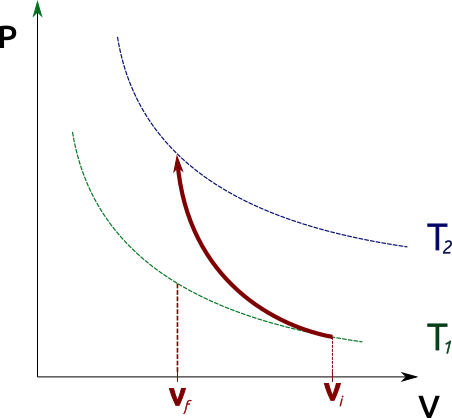
\includegraphics[width=0.7\textwidth]{adiaba.png}
    \caption{Gráfica de un proceso\\ adiabático.}
    \label{Fig. 1.6}
    \end{minipage}
\end{figure}
\vspace{-7mm}

\begin{equation*}
    \Delta U=W\quad;\quad\Delta u=\frac{f}{2}Nk_{B}\Delta T\Longrightarrow\frac{f}{2}Nk_{B}\Delta T=-P\Delta V
\end{equation*}

Expresando $P$ en función de $V$ con la ecuación \ref{Eq. 1.6} resulta en:

\begin{equation*}
    \frac{f}{2}\int_{T_{i}}^{T_{f}}\frac{\mathrm{d}T}{T}=-\int_{V_{i}}^{V_{f}}\frac{\mathrm{d}V}{V}
\end{equation*}

Resolviendo la integral,

\begin{equation}
    \frac{f}{2} \ln \left(\frac{T_{f}}{T_{i}}\right)=\ln \left(\frac{v_{i}}{v_{i}}\right) \rightarrow\left(\frac{T_{f}}{T_{i}}\right)=\left(\frac{v_{i}}{v_{t}}\right)^{2 / f}
    \label{Eq. 1.16}
\end{equation}

La ultima ecuación se puede reescribir,

\begin{equation}
    \begin{split}
        T_{f}V_{f}^{\frac{2}{f}}&=T_{i}V_{i}^{\frac{2}{f}}=cte\\
        P_{f}V_{f}^{\gamma}&=P_{i}V_{i}^{\gamma}\qquad;\qquad\gamma=\frac{2+f}{f}\longrightarrow&&\text{Constante adiabática}\\
    \end{split}
    \label{Eq. 1.17}
\end{equation}

Las cantidades extensivas dependen de la masa, por lo tanto del volumen, las cantidades intensivas no dependen del volumen ni de la masa del sistema, son independientes.

La capacidad térmica se usa bastante y tiene una relación importante con la cantidad de calor.

\begin{equation}
    C=\frac{Q}{\Delta T}\quad\longrightarrow\quad\text{Capacidad térmica}
    \label{Eq. 1.18}
\end{equation}

La ecuación \ref{Eq. 1.18} depende del calor y la temperatura, va a cambiar de temperatura cuando inyectamos calor, además está relacionado con las transiciones de fase. El calor especifico por unidad de masa

\begin{equation}
    c=\frac{C}{n}\quad\longrightarrow\quad\text{Calor específico por unidad de mol}
    \label{Eq. 1.19}
\end{equation}

esta relacionado con el cambio de la energía interna. En un proceso de compresión, se relaciona con el cambio en el volumen del sistema.

\begin{equation*}
    \Delta U=Q-P\Delta V
\end{equation*}

Despejando $Q$ y agregando el término a a ecuación \ref{Eq. 1.18},

\begin{equation}
    C=\frac{\Delta U+P\Delta V}{\Delta T}
    \label{Eq. 1.20}
\end{equation}

Si en el sistema el volumen es constante, tenemos que la capacidad térmica es:

\begin{equation}
    C_{v}=\left(\frac{\partial U}{\partial T}\right)_{V} \quad;\quad U=U(P,T)
    \label{Eq. 1.21}
\end{equation}

La diferencial parcial puede depender de la temperatura o de la presión, depende de las características del sistema. En el caso de un \textbf{gas ideal} la capacidad térmica a volumen constante sería 

\begin{equation}
    C_{v}=\frac{f}{2}Nk_{B}=\frac{f}{2}nR
    \label{Eq. 1.22}
\end{equation}

Según la ecuación \ref{Eq. 1.22} el calor específico a volumen constante es:

\begin{equation*}
    c_{v}=\frac{C_{v}}{mol}=\frac{f}{2}R
\end{equation*}
 
La capacidad térmica a presión constante es:

\begin{equation}
    C_{p}=\left(\frac{\Delta U+P\Delta V}{\Delta T}\right)=\left(\frac{\partial U}{\partial T}\right)_{p}+P\left(\frac{\partial V}{\partial T}\right)_{p}
    \label{Eq. 1.23}
\end{equation}

En la ecuación \ref{Eq. 1.23} hay diferenciales que dependen de otras variables. Cuando se hace un experimento, lo que se hace es variar una variable y ver que pasa con las demás variables. La relación que existe entre $C_{v}$ y $C_{p}$ entre la ecuación \ref{Eq. 1.22} y \ref{Eq. 1.23} es:

\begin{equation}
    C_{p}=c_{v}+p\left(\frac{\partial V}{\partial T}\right)_{p}=\frac{f}{2}nR+nR
    \label{Eq. 1.24}
\end{equation}

En general $C_{p}$ es mayor a $C_{v}$, cuando tenemos presión constante, permitimos que se expanda; cuando tenemos volumen constante no se expande, el calor que entra se convierte en energía térmica y la temperatura aumenta. Cuando inyecto calor, el sistema se expande, por eso $C_{p}$ es mayor a $C_{v}$. Al absorber el calor rápido aumenta su temperatura que se transforma en energía térmica y no va a existir tanta capacidad calorífica, en lo contrario parte del calor se suministra en aumentar la energía a las partículas y aumentar el volumen, capacidad energética $C_{v}$ y capacidad entálpica $C_{p}$. 

\begin{figure}[H]
    \centering
    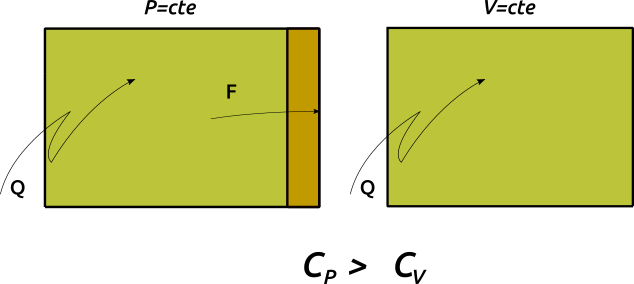
\includegraphics[width=0.8\textwidth]{cpcvbox.png}
    \caption{$C_{v}$ y $C_{p}$ respectivamente.}
    \end{figure}

El nombre de capacidad térmica esta un poco mal dado. Muchos autores lo denominan como capacidad energética porque depende de la energía. Cuando realizamos un proceso isotérmico no tenemos cambio de temperatura, podemos ingresar calor sin cambiar la temperaturas, eso es un cambio de fase, puede pasar de hielo a liquido. Para corregir el problema se introdujo algo llamado \textbf{calor latente} y mide la cantidad de energía de debo administrar a una masa manteniendo su temperatura constante. Es un proceso que pasa a presión constante  y a temperatura constante:

\begin{equation}
    L=\frac{Q}{m}
    \label{Eq. 1.25}
\end{equation}

Cuando se hace este proceso se rompen las ligaciones entre las moléculas, es darle más energía a las partículas que definen el gas.

\begin{example}
Calor latente del agua ($H_{2}O$).

\begin{equation*}
    L_{s-l}=333 \left[\frac{J}{g}\right]\quad;\quad L_{l-g}=2260 \left[\frac{J}{g}\right]
\end{equation*}

El calor latente para pasar de hielo a líquido es mucho menor que el calor latente para pasar de líquido a gas, es decir que se gasta más energía de pasar el agua de liquido a gas que de hielo a líquido. 
\end{example}

Se definen los cambios de fase cuando hay una característica del sistema que cambia drásticamente. Cada sistema debe definir una variable que puede ver que va a cambiar bruscamente cuando cambia otra variable. 

\section{Potenciales termodinámicos}
\subsection{Entalpía}

la capacidad térmica son variables que se pueden medir experimentalmente. Podemos relacionar la capacidad térmica a presión constante con otra cantidad física muy usada y es la entalpía. Por definición la entalpía es un potencial termodinámico o energía libre. Cuando quiero crear un sistema en un volumen en el espacio. ¿Cuanta energía debo tener para crear el sistema? eso representa la entalpía.
\begin{comment}

\begin{figure}[H]
    \begin{minipage}[c]{0.4\linewidth}
        \centering
        \includegraphics[width=0.3\textwidth]{Sdf}
        \caption{Caption}
        \label{Fig. 1.8}
    \end{minipage}
\begin{minipage}[c]{0.4\linewidth}
    \begin{equation}
        H=U+PV
        \label{Eq. 1.26}
    \end{equation}
\end{minipage}
\end{figure}

\end{comment}

El sistema físico creado en la imagen \ref{Fig. 1.8} tiene una energía interna, tengo que darle la suficiente energía para que tenga esa energía. Además tengo que gastar energía para mover las partículas de aire y crear el sistema. Como se ve en la ecuación \ref{Eq. 1.26} es un proceso a presión constante y es la energía que voy a gastar para crear un sistema con cierto volumen en el espacio. Tomando la ecuación \ref{Eq. 1.26} como diferenciales:

\begin{equation}
    \Delta H=\Delta U+P\Delta V
    \label{Eq. 1.27}
\end{equation}

Definíamos en la ecuación \ref{Eq. 1.23} la capacidad térmica a presión contante, prácticamente es la definición de entalpía. Usando \ref{Eq. 1.27}, tenemos que

\begin{equation}
    C_{P}=\left(\frac{\partial H}{\partial T}\right)_{P}
    \label{Eq. 1.28}
\end{equation}

En este caso debe ser una función que depende de la presión y temperatura. Mucha gente denomina a esta capacidad térmica como capacidad entálpica porque mide justamente el cambio de energía con respecto a la temperatura. Al final es una variable termodinámica que se usa porque apenas depende del flujo de energía. El cambio de la entalpía es una variable que no depende del volumen del sistema.

\begin{exercise}
Entalpía de formación\\

Tenemos $\frac{1}{2}$ mol de $H_{2}$ que encontramos fácilmente en la naturaleza. Queremos disociar esa molécula para formar una mol de $H$. ¿Cuanta energía necesitamos gastar a temperatura ambiente ($298 [K]$) y presión atmosférica ($1 [atm]$) para poder disociar esas moléculas y crear la mol de hidrógeno?.

En las tablas aparece la energía entálpica deformación para esta situación, entonces:

\begin{equation*}
    \Delta H=217.97 [kJ]
\end{equation*}

Esa es la energía que necesito gastar para disociar la molécula y formar hidrógeno atómica. Según la ecuación \ref{Eq. 1.27} además de necesitar energía para disociar la molécula, necesito energía para cambiar el volumen, entonces el término $P\Delta V=\Delta nRT$ va a pasar de tener media a una mol. el gasto energético para hacer esa expansión   una mol de hidrógeno es aproximadamente $1.24 [kJ]$. Ahora la energía que necesito para disociar la molécula va despejando $\Delta U$ de la ecuación \ref{Eq. 1.27} es.

\begin{equation*}
    \Delta U=\Delta H-P\Delta V \approx 216.73 [kJ]
\end{equation*}

Ahora, ¿Cuanta energía por mol se gasta? seria:

\begin{equation*}
    \frac{\Delta U}{mol}=\frac{216.73}{\frac{1}{2}6\times10^{23}}\approx7.2\times10^{-19} [J]
\end{equation*}

En electronvolts es $4.49 [eV]$. Se puede medir el cambio de la entalpía experimentalmente, no se puede medir directamente la entalpía en si. Ya hay tablas para casi todos los elementos. 
\end{exercise}

\begin{exercise}
$H_{2}O$ en forma líquida transformar $h_{2}O$ en forma gaseosa. ¿cuanta energía se necesita para hacer esa transformación?. \\

Hay que buscar el calor latente del agua en estado líquido a temperatura constante y presión constante. La transición de fase acontece cuanto se esta a $100[K]$ a $1 [atm]$. Una mol de agua en fase líquida y fase gaseosa pesan lo mismo ($18 [g]$), lo que cambia es el volumen que es mayor e fase gaseosa. En las tablas aparece el valor $\Delta H=40660 [J]$, entonces ¿cuanta energía necesito?. En la ecuación \ref{Eq. 1.25} esta la respuesta, el calor latente es la energía que necesito para hacer esta transformación. Como es a presión constante es proporcional a la entalpía:

\begin{equation*}
    L=\frac{\Delta H}{18 [g]}=2260 [\frac{J}{g}]\sim540[\frac{cal}{g}]
\end{equation*}

Este es el calor que se necesita para romper as interacciones. La energía que se gastó para aumentar el volumen es:

\begin{equation*}
\frac{P\Delta  V}{18 [g]}=\frac{nRT}{18 [g]}=\frac{3100 [J]}{18 [g]}    
\end{equation*}

Esta es la energía para expandir una mol de agua y pasar de fase líquida a fase gaseosa. 
\end{exercise}

\section{Fenómenos de transporte}

Seguimos usando la teoría cinética de los gases que es un modelo mecánico microscópico para definir propiedades macroscópicas. Es una teoría que esta bastante relacionada con la probabilidad. Los mecanismos de transferencia que se hablaron en la sección 1.3.1 son fundamentales es este fenómeno. Decíamos que la conducción se debe al contacto microscópico, que la convección se debe a un movimiento global, y la radiación que depende de las ondas electromagnéticas. Los dos últimos procesos son difíciles de modelar con un modelo simple, pero el proceso de conducción si esta relacionado con la teoría cinética. 

\subsection{Conductividad térmica}

Un ejemplo de fenómeno de transporte es lo que se conoce como conducción térmica. Tenemos un sistema exterior e interior con diferentes tempera rutas, pero $T_{2}>T_{1}$, lo mas probable que suceda es que ese sistema transmita energía. La cantidad de calor que transferimos depende las condiciones para esa transferencia. La cantidad de calor que podemos transferir de un sistema a otro va a depender de diferentes variables. Cuando se deja el café en el termo dejamos que exista un tiempo de relajación $\Delta t$. Si el $\Delta T$ es muy grande, va a aumentar la cantidad de calor que sale del sistema, esa cantidad de calor que va a salir depende del espesor $\Delta x$ de la pared térmica:
\begin{comment}

\begin{figure}[H]
    \begin{minipage}[c]{0.4\linewidth}
        \centering
        \includegraphics[width=0.3\textwidth]{Sdf}
        \caption{Caption}
        \label{Fig. 1.8}
    \end{minipage}
\begin{minipage}[c]{0.4\linewidth}
    \begin{equation}
        Q\propto\frac{\Delta tA\Delta T}{\Delta x}
        \label{Eq. 1.29}
    \end{equation}
\end{minipage}
\end{figure}

\end{comment}
Lo que se confirma experimentalmente es que la cantidad de calor por unidad de tiempo es proporcional a las variables de la ecuación \ref{Eq. 1.29}, esa constante de proporcionalidad es lo que se conoce como conductividad térmica.

\begin{equation}
    \frac{Q}{\Delta t}=-K_{t}A\left(\frac{\partial T}{\partial x}\right)
    \label{eq. 1.30}
\end{equation}

Entre mayor área mayor transferencia de calor, esta es la ley de Fourier. La constante $K_{J}$ se mide para diferentes sistemas como el aire ($0.026$), la madera ($0.08$), el vidrio ($0.8$), el hierro ($80$) o el cobre ($400$) con unidades de $\frac{J}{msK}=\frac{Watt}{ms}$. La conductividad térmica esta relacionada con las vibraciones de la red, por eso es tan complicada la transferencia de energía en la madera o el vidrio. El cobre es mayor que el hierro porque además de transferir energía térmica por los fonones, también porque los electrones de conducción ayudan a aumentar esa energía térmica. La conductividad térmica esta relacionada directamente con la conductividad eléctrica.

\begin{example}
Conductividad térmica de un gas\\
%imagen
El gas va a tener al equilibrio, quiere decir que se transfiere energía por contacto microscópico. Las moléculas que hacen esa transferencia de energía son las que viven en la regiones de frontera, las de la derecha se mueven a la izquierda y viceversa. la cantidad de energía que se transfiere es, como estamos considerando un gas ideal, un sistema que no se expande, por o tanto la energía interna del sistema va a depender de la cantidad de calor que se transfiere:

\begin{equation*}
    Q=\frac{1}{2}U_{1}-\frac{1}{2}U_{2}
\end{equation*}

Como es el mismo gas en ambos lados,

\begin{equation*}
    Q=-\frac{C_{v}}{2}\Delta T
\end{equation*}

La mitad de las partículas con temperatura $T_{1}$ se van hacia la derecha y la mitad de las partículas con temperatura $T_{2}$ se van hacia la izquierda. La partícula azul debió recorrer una cierta distancia antes de entregar esa energía, igual pasa con la partícula roja. La distancia que recorre antes de chocar es conocido como camino libre medio $l=\Delta x$.  
\end{example}

De forma general, el calor transferido es:

\begin{equation}
    Q=-K_{t}A\Delta  t\left(\frac{\partial T}{\partial x}\right)
    \label{Eq. 1.31}
\end{equation}

Para un gas ideal encontramos que:

\begin{equation}
    Q=-\frac{1}{2}C_{V}\Delta x\left(\frac{\partial T}{\partial x}\right)
    \label{Eq. 1.32}
\end{equation}

Comparando la ecuación \ref{Eq. 1.32} con la ecuación \ref{Eq. 1.31} podemos deducir que:

\begin{equation}
    K_{t}=\frac{1}{2}\frac{C_{V}\Delta x}{A\Delta t}
    \label{Eq. 1.33}
\end{equation}

La velocidad media de las partículas esta relacionada con $\frac{l}{\Delta T}$ y es proporcional a la temperatura. 

\begin{equation*}
    v_{med}\propto\sqrt{T}
\end{equation*}

Si reemplazamos esa idea en la ecuación \ref{Eq. 1.33} obtenemos:

\begin{equation}
    K_{t}=\frac{1}{2}\frac{C_{V}}{A}\frac{\Delta x}{\Delta x}v_{med}
    \label{Eq. 1.34}
\end{equation}

La capacidad térmica para un gas ideal $K_{t}\propto Vv{med}\propto\sqrt{T}$. Esta ley es llamada ley Fick. Esto se demostró experimentalmente para diferentes gases con densidad baja para poder considerarlo un gas ideal. El camino libre medio se puede calcular de la siguiente manera.

%imagen

Dos moléculas se van a encontrar cuando sus centro se encuentren a $2R$. Puedo considerar que la molécula tiene un volumen igual a $4R$ con longitud $l$. Si otra partícula entra en ese volumen vana transferir energía. Cuando el volumen esta sobre la molécula, corresponde al volumen total dividido entre el número de partículas, existe la colisión cuando:

\begin{equation*}
    \pi(2R)^{2}l=\frac{V}{N}
\end{equation*}

El libre camino medio queda definido como:

\begin{equation}
    l=\frac{V}{N}\frac{1}{4\pi R^{2}}
    \label{Eq. 1.35}
\end{equation}

La interpretación física de la ecuación \ref{Eq. 1.35} es que cuando aumento el volumen del sólido, aumento el libre camino medio de las partículas, entre más partículas le aumenta al sistema mayor probabilidad hay de que colisionen. Si fuera un gas ideal ($PV=nk_{B}T$), el camino libre medio es:

\begin{equation}
    l=\frac{k_{B}T}{P4\pi R^{2}}
    \label{Eq. 1.36}
\end{equation}

cuando aumento la temperatura aumento el camino libre medio, cuando aumento la presión disminuye el camino libre medio. El modelo de gas ideal si describe un sistema de baja densidad de partículas, esto lo confirmó la ley de Fick.

\subsubsection{Viscosidad}

La viscosidad es una fuerza de arrastre que se opone al movimiento en un determinado fluido. Va ser proporcional a la diferencia de momento que hay en el sistema. Las partículas que están cerca a la placa van a querer moverse a la misma velocidad de la placa, las partículas que están pegadas a esta partículas no va a dejar hacerlo, lo que determina la fuerza de arrastre. Esa fuerza va a ser proporcional al área de la placa, a medida que aumentamos el grosor de la placa, la fuerza de arrastre tiene que disminuir.

\begin{equation*}
    F\propto A\frac{\Delta U}{\Delta z}
\end{equation*}
%imagenadhtyuhijhjgfdss

Entonces,

\begin{equation}
    \frac{F_{x}}{A}=\eta\frac{\mathrm{d}U}{\mathrm{d}z}
    \label{Eq. 1.37}
\end{equation}

Donde $\eta$ es la constante de proporcionalidad. En la ecuación \ref{Eq. 1.37} no tenemos una presión como tal, es una fuerza sobre un área, pero la presión no esta aplicada perpendicularmente al área, entonces no corresponde a una presión, esta fuerza se denomina fuerza de cizallamiento. El tensor de estrés esta formado en la diagonal por las presiones que definimos perpendiculares, y las fuerzas de cizallamiento son las que no están en la diagonal del tensor de estrés y que dependen de la viscosidad del sistema. Como conclusión esa viscosidad $\eta$ para los gases ideales depende como $\sqrt{T}$ porque si aumento la densidad de partículas, disminuyo la velocidad con la que se transfiere la energía.

\subsection{Conductividad eléctrica}

Suponemos que tenemos electrones que se mueven a través de una malla. Los electrones libres son electrones que están débilmente ligados a la red cristalina, tienen la característica que cualquier perturbación los deja libre y se convierten en electrones de conducción para generar corriente eléctrica. Un ejemplo de perturbación es colocarle n campo eléctrico, todos se van a mover con una velocidad e arrastre, también s le aumentamos la temperatura, los electrones se pueden soltar de sus átomos y andar libremente. La velocidad de estas partículas es proporcional a $\sqrt{T}$. A partir de esto podemos definir la carga o la densidad de corriente:

%imagen
\begin{equation}
    \begin{split}
        q&=en_{e}AU\Delta t\\
        J&=\frac{q}{A\Delta t}=en_{e}v
    \end{split}
    \label{Eq. 1.38}
\end{equation}

La velocidad depende del campo eléctrico, esa velocidad de arrastre depende de la aceleración por el tiempo promedio antes de hacer una colisión. 

\begin{equation}
    \bar{v}=at=\frac{eE}{m}t
    \label{Eq. 1.39}
\end{equation}

Entonces la densidad de corriente la podemos definir como:

\begin{equation*}
    J=\frac{e^{2}n_{e}t}{m}E
\end{equation*}

Denominamos $\frac{e^{2}n_{e}t}{m}$ como conductividad térmica, entonces:

\begin{equation}
    \Vec{J}=\sigma\Vec{E}
    \label{Eq. 1.40}
\end{equation}

La densidad de corriente va a depender del campo eléctrico aplicado y de la conductividad térmica.

Esto hace parte más del curso de estado sólido.

%%%%%%%%%%%%%%%%%%%%%%%%%%%%%%%%%%%%%%%%%%%%%%%%%%%%%%%%%%

\chapterimage{band1.png}
\chapter{Ensambles}

\section{Preliminares}

Tenemos un sistema de tres monedas, ¿De cuántas formas puedo tener una distribución de cara y sello?

\begin{table}[H]
    \centering
    \begin{tabular}{c c c }
    \hline\hline
    100   & 200 & 500 \\\hline
    c     & c   & c\\
    c     & c   & s\\
    c     & s   & c\\
    s     & c   & c\\
    s     & s   & c\\
    c     & s   & s\\
    s     & c   & s\\
    s     & s   & s\\
    \end{tabular}
    \caption{Posible microestados de un sistema de tres monedas indistinguibles que solo pueden tener dos estados cada una, cara y sello.}
    \label{Tab. 1}
\end{table}

En la tabla \ref{Tab. 1} se muestran los posibles estados que muestra el sistema, el posible número de estados que voy a conseguir, en total son 8 posibles configuraciones que tienen el sistema donde cada moneda tiene dos estados posibles. A cada uno de los 8 estados del sistema se les conoce como un microestados. 

Podemos ver que hay un estado que tiene 3 caras, hay otro conjunto de estados que tiene dos caras, hay otro conjunto que tiene una cara y hay un último conjunto que tiene cero caras. Podemos definir dentro de ese conjunto de posibles resultados, subconjuntos que tienen una característica en común. Con ese conjunto de microestados podemos formar subgrupos con características comunes, a esos subconjuntos lo llamamos como macroestados. Un macroestado esta formado por microestados. 

\begin{definition} [Multiplicidad ($\Omega$)]
Los macroestados pueden tener diferente multiplicidad. Se le conoce como multiplicidad la cantidad de microestados que un macroestado puede tener. La suma de todas las multiplicidades para cada macroestado resulta en el número total de microestados.

\begin{equation}
    \Omega_{T}=\sum\Omega_{i}
    \label{Eq. 2.1}
\end{equation}
\end{definition}

\begin{example}
El macroestado que tiene tres cara tiene una multiplicidad de $\Omega(3c)=1$. La multiplicidad del macroestado con dos cara y una cara $\Omega(2c)=\Omega(2c)=3$. El macroestado con cero caras tiene multiplicidad $\Omega(0c)=1$. La multiplicidad total es $\Omega_{T}=8$.

La multiplicidad define las propiedades termodinámicas del sistema.
\end{example}

Hablando de probabilidad, la probabilidad de obtener un microestado que pertenece al macroestado \textit{(3c)}, pues es $P(3c)=\frac{1}{8}$, la probabilidad de obtener el macroestados \textit{(2c)} es $P(2c)=\frac{3}{8}$, la probabilidad de obtener \textit{(1c)} es $P(1c)=\frac{3}{8}$, la probabilidad de obtener \textit{(0c)} es $P(0c)=\frac{1}{8}$. Si tengo el sistema de tres moneda y hago bastantes intentos, el macroestado mas probable que puedo obtener es que mi sistema se encuentre en el macroestado \textit{(2c)} o \textit{(1c)}. No se sabe en cuál microestado, pero se sabe que el sistema pueda resultar dos monedas con dos caras o dos monedas con una cara. 

\begin{definition}[Principio fundamental de la estadística]

Al definir la probabilidad en función de la multiplicidad sobre el número total de microestados, estoy definiendo que todos los microestados de un sistema son igual de probables. No hay razón para darle mayor probabilidad a un microestado que a otro.
\end{definition}

En el caso de tener $100$ monedas, ¿Cuantos macroestados va a tener el sistema?. Los macroestados corresponden a los conjuntos que puedo obtener. El primer conjunto es que todas las monedas caigan en cara hasta llegar a un conjunto donde no voy a tener ninguna cara.

\begin{equation*}
    cccc...c(100)\quad;\quad cccs...c(100)\quad;\quad cscs...c(100)\quad;\quad scsc...s(100)\quad;\quad ssss..s(100)
\end{equation*}

El número de macroestados en este caso se puede definir como el número de elementos en el sistema. La multiplicidad $\Omega(100c)=1$, existe simetría en el sistema donde la multiplicidad $\Omega(0c)=1$. La multiplicidad $\Omega(99c)=100$, porque el sello se puede mover entre los $100$ elementos. La multiplicidad de $\Omega(98c)=\frac{100\cdot99}{2}$ Porque el primer sello se puede mover en cualquier posición, entonces tiene $100$ posibilidades, pero el segundo va a tener $99$ posibilidades debido a que está acompañado de otro sello que ocupa un lugar. Como consideramos monedas indistinguibles, se deben contar el número de permutaciones, entonces de ese conjunto hay unos que se repiten y no se pueden considerar microestados diferentes, en este caso se repiten dos configuraciones. 

Cuando existe un macroestado con $97$ caras, la multiplicidad es $\Omega(97c)=\frac{100\cdot99\cdot98}{3!}$. Permutaciones indistinguibles son tres. En este caso para un macroestado con $n$ caras es:

\begin{equation*}
    \Omega(nc)=\frac{100\cdot99\cdot98...(n+1)}{(100-n)!}
\end{equation*}

En una forma mas general:

\begin{equation}
    \Omega(n)=\frac{N!}{(N-n)!n!}=\binom{N}{n}
    \label{Eq. 2.2}
\end{equation}

La ecuación \ref{Eq. 2.2} representa el número de configuraciones que puede tener el sistema que tienen $n$ caras. Me dice la cantidad de microestados que voy a tener asociado a un macroestado con $n$ caras.

%imagen gráfica aguss

Existe un macroestado que es el mas probable, definiendo la probabilidad de ese macroestado como:

\begin{equation}
     P(\Omega)=\frac{\Omega(n)}{\Omega_{T}}
     \label{Eq. 2.3}
\end{equation}

\section{Ensamble en equilibrio}

El primero en hablar de ensamble fue Gibbs en 1902, lo definió como una colección de macroestados, un conjunto de réplicas del sistema. 

%imagen ensamles

Un ensambles puede estar formado por un macroestado, o dos o $n$ macroestados. La característica de un ensamble es que tienen que ser formado por réplicas de un sistema real. La probabilidad de encontrar el microestado es la mismo. El ensamble no necesariamente contiene todos los microestados.

Cuando decimos que existen diferentes tipos de ensambles, lo que se esta haciendo es que se le ponen constricciones a esos ensambles. Cuando se habla de ensamble canónico se dice que todos los ensambles tienen algo en común.

\subsection{Ensamble microcanónico (NVE)}

La colección de macroestados dentro del ensamble se encierra adiabáticamente, no se permite que entre o salga energía en forma de calor o trabajo. Esto implica que la energía de ese ensamble va a ser una constante. No puedo tener intercambio de energía con el ambiente.

%imagen adiabatico

Ese sistema tampoco puede intercambiar partículas o estados. El ensamble tiene un número de réplicas del sistema físico, como está aislado, el número de microestados en el ensamble no va a cambiar. Tampoco puedo cambiar el volumen, es decir es una constante. El ensamble es microcanónico si cumple estas tres condiciones $N=V=E=cte$.

Para cada macroestado que hace parte del ensamble, le podemos asociar una probabilidad y una energía, lo que tenemos que garantizar que la energía total del ensamble sea una constante. Puede haber transferencia de energía entre dos macroestados, pueden interactuar y va a cambiar una redistribución de la energía, pero no debe modificar la característica del macroestado. Si un macroestado pierde energía, otro macroestado debe ganarla para que la energía permanezca constante.

En sistemas físico vamos a hablar de microestados, macroestados, multiplicidad y ensambles.

\begin{example}[Paramagnético de dos estados]

Tenemos un material con momentos magnéticos que se alinean con un campo magnético externo. Cuando se apaga el campo magnético pierde la magnetización, los momentos magnético se desordenan. Como consecuencia de la cuantización del momento magnético, este va a tener dos estados, espín 'up' y espín 'down'. 

%imagen ferro para

Cuando colocamos el campo magnético, el número de momentos magnéticos que se alineen con el campo va a ser mayor que los momentos magnéticos que se alineen en contra del campo magnético. El microestado en este caso es la posición de cada momento magnético. El número espines 'up' es $N_{\uparrow}=5$, ¿Cuantas configuraciones diferentes con 5 espines 'up' podría tener?. Los espines 'down' se pueden distribuir en el número total de elementos. Voy a tener asociado un conjunto de posibles configuraciones donde van a haber 5 espines 'up'.

%imagen 5

El macroestado lo definido en función del número total de espines 'up'. Como el sistema es finito, $N=N_{\uparrow}+N_{\downarrow}$, esto debe ser una constante. La energía de un espín 'down' es mayor a la energía del espín 'up' porque debe darle energía al sistema para ir en contra del campo magnético. La multiplicidad se calcula con la ecuación \ref{Eq. 2.2}:

\begin{equation*}
    \Omega(N_{\uparrow})=\frac{N!}{N_{\uparrow}!N_{\downarrow}!}
\end{equation*}

La multiplicidad define las propiedades termodinámicas del sistema, a cada macroestado se le asocia una energía, esa energía depende de cuantos espines tengo o no alienados al campo magnético. Entre mas espines en contra del campo, mayor va a ser la energía del sistema. Cuando se introduce temperatura en el sistema, los espines tienden a desalienarse. Hay una competencia entre el campo magnético y la temperatura. 

%imagen

Si tenemos altos campos magnéticos y bajas temperaturas, el efecto del campo magnético va a ser mayor y ocurre un alineamiento con el campo. Si se tiene temperaturas altas y bajos campos magnéticos, lo que se obtiene es que el número de espines hacia arriba va a ser aproximadamente el número de espines hacia abajo.

\end{example}

La multiplicidad esta directamente relacionada con la energía del sistema y con otras propiedades termodinámicas. Si la multiplicidad de un macroestado es muy alta su energía va a ser menor que un sistema con multiplicidad baja.


\subsection{Sólido de Einstein}

Es un ejemplo de un ensamble microcanónico.  La idea es explicar porque la capacidad térmica en metales tiende a cero. En metales el calor no va a depender de cambios en el volumen porque no se expande ni se comprime, la energía interna depende del calor que le suministremos al objeto. Un sólido es un conjunto de osciladores con dos grados de libertad, uno de energía cinética y otro de energía potencial. Ese conjunto de osciladores deberían tener una energía térmica, entonces:

%%%%%%%%%%%5image minipage

\begin{equation}
    U=2N\frac{1}{2}K_{B}T
    \label{Eq. 2.4}
\end{equation}

En el conjunto de osciladores, la capacidad térmica la definimos a volumen constante, es decir la energía interna no va a cambiar por algún trabajo de compresión, solo de calor:

\begin{equation*}
    C=\left(\frac{\partial U}{\partial T}\right)_{V}\cong NK_{B}=nR
\end{equation*}

Experimentalmente se veía que sí pasaba esto, pero había un caso especial. La mayoría de los sólidos tenia una capacidad térmica de $\frac{3}{2}nR$:


%%%imagen


Había un caso especial, a $25 [K]$ el diamante no seguía la ley de Lyon-Petit, la capacidad térmica de un sólido debe ser justamente $\frac{3}{2}nR$. Lo que propuso Einstein es que el diamante debe tener una constante elástica muy grande que hace que no respete esa ley, entonces el diamante debe tener efectos cuánticos.Postuló que esos sólidos no necesariamente son sólidos clásicos, deben estar formados por osciladores cuánticos. Él introduce un modelo donde consideramos que a cada oscilador que forma el sólido los puedo describir a través de un oscilador cuántico. La capacidad térmica del sólido tiende a ser cero cuando disminuimos la temperatura.

%%%%%%%%%%%%%%%%%%%%%imagen minipage

\begin{equation}
    E_{n}=\hslash\omega\left(n+\frac{1}{2}\right)
    \label{Eq. 2.5}
\end{equation}

En base a esta idea, los osciladores van a tener su energía discretizada, van a tener un número discreto de estados, esa energía depende de la frecuencia de oscilación (ecuación \ref{Eq. 2.5}). Los osciladores pueden interactuar entre ellos de forma débil sin alterar los osciladores, pero una interacción suficientemente grande para intercambiar energía. Como hay una constante en el cambio de energía, $\Delta E=\hslash\omega$, redefinimos el cero del sistema, ahora es $E_{0}=\frac{\hslash\omega}{2}=0$. Como se ve en la imagen %\ref
es que la energía del primer oscilador es $E_{1}=\hslash\omega q_{1}$, el segundo oscilador podría tener una energía $E_{2}=\hslash\omega q_{2}$, para todos los osciladores voy a tener una energía asociada a los cuantos de energía que le estoy suministrando a los osciladores. Como es un ensamble microcanónico, la energía total no va a entrar ni salir calor, no se va a ver modificada. La energía del ensamble es la suma de cada uno de los osciladores. 

\begin{equation}
    E_{T}=\sum E_{i}=\hslash\omega\sum q_{i}=\hslash\omega q=cte
    \label{Eq. 2.6}
\end{equation}

El macroestado estaría formado por $N$ osciladores y una energía $q$. La energía del sistema puede ser distribuida por los osciladores. Tengo varias formas de distribuir esa energía en los microestados. El macroestado del sólido va a depender de cuantos osciladores tengo y la energía interna del conjunto de osciladores. Si tenemos cuatro osciladores como en la imagen %%\ref
Tenemos $N=4$ y vamos a distribuir $q=8$, es decir tenemos 8 cuantos de energía que van a ser distribuidos en 4 osciladores. ¿Cual sería la multiplicidad $\Omega(N,q)$ del sistema?. Podemos distribuir en los niveles de energía los cuantos de energía de diferentes maneras.

%%%%%%%%%%%%imagen

Para encontrar las diferentes formas de distribución de la energía en los osciladores, se coloca una barra en medio de los osciladores y se cuentan junto con las barras los elementos en el sistema. Para este caso es $11$. Lo que hacemos es distribuir en 11 cajas las tres barras que colocamos. El problema se reduce a una combinatoria (ecuación \ref{Eq. 2.2}) donde tengo que acomodar tres líneas en 11 cajas. Es un método para entender el problema. La multiplicidad de ese macroestado $\Omega(N.q)$ depende del total de elementos mas el número total de osciladores menos 1:

\begin{equation}
    \Omega(N,q)=\frac{\left[(N-1)+q\right]!}{(N-1)!q!}
    \label{Eq. 2.7}
\end{equation}

La ecuación \ref{Eq. 2.7} nos dice de cuantas formas puedo repartir $q$ cuantos de energía en $N$ osciladores. La multiplicidad depende del número de osciladores y la energía a distribuir. Para este caso:

\begin{equation*}
    \Omega(4,8)=\frac{\left[(4-1)+8\right]!}{(4-1)!8!}=165
\end{equation*}

Esto quiere decir que vamos a tener 165 formas de distribuir 8 cuantos de energía en 4 osciladores. Lo importante es calcular la multiplicidad. 

\section{Interacción térmica}

Con la idea del sólido en Einstein se va a intentar explicar porque fluye la energía, realmente es un efecto probabilístico  da una idea de porque estos procesos son irreversibles. Como prohibimos que entre y salga energía del sistema, la energía total del sistema es una constante, pero puedo intercambiar energía. La energía y la multiplicidad la definimos como:


%%%%%%%%%imagen imnipage

\begin{equation}
    E=E_{A}+E_{B}=cte\quad;\quad\Omega_{T}=\Omega_{A}\cdot\Omega_{B}
    \label{Eq. 2.8}
\end{equation}

La otra condición es el tiempo de transferencia entre macroestados sea mucho mas lenta que la velocidad que tiene el sólido para llegar al equilibrio. Vamos a tener una distribución de energía entre los dos sólidos. Cada uno de os sólidos se componen de 3 osciladores, es decir un total de seis osciladores; tenemos también 6 cuantos de energía para distribuirlos en los osciladores de los dos sólidos. Tenemos en el sistema $N_{A}=N_{B}=6$ con $q=6$.

\begin{table}[H]
    \centering
    \begin{tabular}{c c c c c}
    \hline\hline
    $q_{A}$ &   $\Omega_{A}$    &   $q_{B}$ &   $\Omega_{B}$  &  $\Omega_{T}$\\
    \hline
     0  &   1   &   6   &   28  &   28  \\
     1  &   3   &   5   &   21  &   63  \\
     2  &   6   &   4   &   15  &   90  \\
     3  &   10  &   3   &   10  &   100 \\  
     4  &   15  &   2   &   6   &   90  \\
     5  &   21  &   1   &   3   &   63  \\  
     6  &   28  &   0   &   1   &   28  \\
    \end{tabular}
    \caption{Distribución de cuantos de energía en los sistemas $A$ y $B$ con su multiplicidad y la multiplicidad total.}
    \label{tab:my_label}
\end{table}

El estado $q_{A}=q_{B}=3$ tiene la mayor multiplicidad, es decir que lo mas probable es que el sistema se encuentre en ese estado. La energía de ese estado tiende a ser igual en los dos sólidos, tiende a favorecer el sistema que equilibre las energías. Si colocáramos su sistema inicial $q=6$ y dejamos un tiempo bastante grande, después de volver a medir, lo mas probable es que el estado mas probable sea $q_{A}=q_{B}=3$, es decir que cada sólido tenga la misma energía. El estado va a entrar en equilibrio, el estado se encuentra en el macroestado  mas probable. Cuando dejamos evolucionar el sistema, el fenómeno probabilístico hace que tenga la misma energía y por ende la misma temperatura, en otras palabras el sistema $A$ y el sistema $B$ tienen a misma temperatura.

Todos los microestados del ensamble tienen la misma probabilidad. Esto implica que no solo tenemos un flujo de multiplicidades, si no también tenemos un flujo de estados. AL final del equilibrio, las energías de los sistemas van a ser iguales porque van a estar en el estado mas probable.


\begin{example}[Multiplicidades altas]
%%%imagen del libro
%%%%%%%5minipage image picos

Ahora se ve un pico de la distribución mas acentuado, entre mas osciladores, mas acentuado va a ser el pico El macroestado mas probable pasa cuando $q_{A}=60$, la multiplicidad esta del orden de $10^{114}$, y un es un sistema pequeño con $N_{A}=300$ y $N_{B}=200$ osciladores. En un sistema real vamos a tener osciladores de número de Avogadro. El macroestado mas probable es $q_{A}=60$ y $q_{B}=40$, lo que indica una energía diferente, pero esto es debido a la deferencia del número osciladores $N$ entre los sistemas. La densidad de energía es lo importante.

\begin{equation*}
    \frac{N_{A}}{q_{A}}=\frac{300}{60}=5=\frac{200}{40}=\frac{N_{B}}{q_{B}}
\end{equation*}

Esa densidad de energía si va a ser igual. Si la condición inicial del sistema es $q_{A}=0$, e sistema va a tender a ir al macroestados mas estable, voy a tener la misma densidad de energía. EL flujo de calor es un fenómeno probabilístico. Si tengo este sistema y quiero hacer una medida, encontrar la probabilidad de que el sólido $A$ tenga una energía menor que 30 $q_{A}<30$, va a ser de aproximadamente $10^{-6}$. de un millón de medidas que realice, solo una me dice que ese sistema tienen una energía menor que 30.
\end{example}

Los sistemas evolucionan a partir de una condición inicial, y evolucionan al macroestado mas probable y ese macroestado tiene la característica de que la densidad de energía va a ser igual,  y eso acontece espontáneamente. Al decir que todos los microestados son igualmente probables, existe una probabilidad que empiece desde macroestado mas probable pero que en algún momento llegue al macroestado menos probable porque estoy considerando que la probabilidad de ir de una  macroestado a otro no tiene ninguna restricción, eso es lo que se conoce como balance detallado. No hay ninguna prohibición, pero el sistema va a tender al estado mas probable y es el que equilibra la energía y por ende la temperatura.

El macroestado mas probable es el que tiene asociada la mayor multiplicidad, hay mas microestados, homogeneiza la temperatura, la energía de todos los elementos va a ser la misma. La entropía es un medida de la multiplicidad. la segunda ley dice que un sistema evoluciona a un macroestado con mayor multiplicidad, evoluciona al macroestado con mayor probabilidad, en otras palabra un sistema evoluciona a estado de máxima entropía.

\begin{definition}[]Segunda ley de la termodinámica]
Cualquier sistema se va a encontrar en equilibrio cuando el sistema este en su estado mas probable.

Generalmente hablamos de la segunda ley en relación con la entropía, el sistema evoluciona a un sistema de mayor entropía. Esta determinado cuando encontramos el macroestado con mayor multiplicidad. El flujo de energía que llamamos calor es un fenómeno probabilístico, lo que identificamos es que el sistema se va a detener cuando las temperaturas sean iguales. En ese momento vamos a encontrar el macroestado mas probable, que lo caracteriza una distribución homogénea de la energía.
\end{definition}

Inicialmente esta ley no fue abordada desde este punto de vista, a finales del siglo $XIV$ se estableció esta relación. El concepto de entropía fue postulada por Carnot diciendo que la entropía es una cantidad que siempre va a aumentar. Se estableció una relación con el mundo microscópico. En el ensamble microcanónico, lo fundamental es calcular la multiplicidad, y con ello calcular las propiedades termodinámicas del sistema. El flujo de energía tiende a equilibrar la temperatura es un fenómeno probabilístico. 

\chapter{Estadística de números grandes}

Consideramos un numero grande del orden del numero de Avogadro $10^{23}$. Un numero pequeño podría ser $100$ o $1000$. Números muy grandes serian potencias de números grandes $[10^{10}]^{23}$. Cuando calculamos la multiplicidad del sistema, vana  aparecer factoriales de esos números $10^{23}!$. Se hace necesario trabajar o establecer una manera de trabajar con esos números que consideramos grandes. 

\begin{definition}[Fórmula de Stirling]
Es una manera de expresar los números factoriales, los podemos expresar mediante la aproximación:

\begin{equation}
    N!\simeq\left(\frac{N}{e}\right)^{N}\sqrt{2\pi N}
    \label{Eq. 3.1}
\end{equation}

Podemos expresar un numero muy grande en función de un numero grandes $(\frac{N}{e})^{N}$ multiplicada por un numero pequeño $\sqrt{2\pi N}$.

Si $N$ es muy grandes, la ecuación \ref{Eq. 3.1} se puede escribir de la forma:

\begin{equation}
    N!\simeq\left(\frac{N}{e}\right)^{N}
    \label{Eq. 3.2}
\end{equation}

El otro término es muy pequeño comparado con la ecuación \ref{Eq. 3.2}. Si consideramos $N=100$, entonces:

\begin{equation*}
    \frac{N!-\left(\frac{N}{e}\right)^{N}}{N!}\approx0.0083
\end{equation*}

A mediad que aumentamos $N$, la formula es mas precisa. Si tomamos:

\begin{equation}
    ln(N!)=Nln(N)-N
    \label{Eq. 3.3}
\end{equation}

Esta expresión se conoce como la formula de Stirling
\end{definition}

\section{Demostración "no formal " de la formula de Stirling}

Podemos expresar en numero factorial como $N!=N(N-1)(N-2)...1$. Si tomamos el $ln(N!)$:

\begin{equation*}
    ln(N!)=ln(N)+ln(N-1)+...+...ln(1)
\end{equation*}

Al hacer la suma del logaritmo natural, se hacen unas sumas. Nos representa el área bajo la curva del $Ln(N!)$, DE forma integral se puede ver que:


%%%%%%%%%%%%%%%%%%%%minipage    imagw
\begin{equation*}
    ln(N!)=\int_{1}^{N}ln(x)dx=xln(x)-x|_{1}^{N}=Nln(N)-N+1
\end{equation*}

El término $+1$ se puede despreciar debido a que $N$ es un numero grande. Suponiendo números muy grandes, entonces:

\begin{equation*}
    ln(N!)=Nln(N)-N
\end{equation*}

Como vamos a trabajar con sistemas de muchas partículas, usamos esta aproximación (\ref{Eq. 3.3}).

\section{Solido de Einstein macroscópico}

Para el solido de Einstein, veíamos que para un determinado macroestado con $\Omega(N,q)$ podíamos calcular la multiplicidad del sistema realizando la combinatoria de la ecuación \ref{Eq. 2.7}. cuando hablamos de números grandes, el $1$ en esta formula es muy pequeño, así que la podemos expresar como:

\begin{equation}
     \Omega(N,q)=\frac{\left[(N+q\right]!}{(N)!q!}
     \label{Eq. 3.4}
\end{equation}

Analizar ese factorial es algo complicado, pero podemos sacar el logaritmo natural de la multiplicidad \ref{Eq. 3.4} y usando la formula de Stirling, tenemos que:

Convirtiendo esos números muy grandes en números grandes, la expresión \ref{Eq. 3.5} la podemos expresar con ayuda de la formula de Stirling:

\begin{equation}
\begin{split}
    ln(\Omega(N,q))&=ln(N+q)!-ln(N!)-ln(q!)\\
    &=(N+q)ln(N+q)-(N+q)-Nln(N)+N-qln(q)+q\\
    ln(\Omega(N,q))&=(N+q)ln(N+q)-Nln(N)-qln(q)
\end{split}
        \label{Eq. 3.5}
\end{equation}

También debemos hablar de temperatura y la energía del sistema. Cuando hablamos de altas temperaturas, nos referimos a que $\frac{q}{N}>>1$, o también $\frac{N}{q}<<1$. En latas temperaturas se introduce esta condición. Podemos introducir esta condición como:

\begin{equation*}
    ln(N+q)=ln\left[q\left(1+\frac{N}{q}\right)\right]=ln(q)+ln\left(1+\frac{N}{q}\right)
\end{equation*}

Esta ultima expresión podemos expandir el ultimo término en Taylor con la aproximación de $ln(1+x)\approx x$ cuando $x<<1$, entonces la anterior ecuación queda:

\begin{equation*}
    ln(N+q)=ln(q)+\left(\frac{N}{q}\right)
\end{equation*}

Volviendo a la ecuación \ref{Eq. 3.5}, el solido de Einstein a altas temperaturas va queda de la forma:

\begin{equation}
    \begin{split}
    ln(\Omega(N,q))&=(N+q)\left[ln(q)+\left(\frac{N}{q}\right)\right]Nln(N)-qln(q)\\
    ln(\Omega(N,q))&=Nln(q)+N-Nln(N)
\end{split}
        \label{Eq. 3.6}
\end{equation}

Ahora es mas facial calcular la multiplicidad del solido de Einstein macroscópico. Como vamos a trabajar con números grandes, mas no muy grandes, podemos tomar la exponencial de la ecuación \ref{Eq. 3.6}:

\begin{equation}
    \Omega(N,q)= e^{ln\left(\frac{q}{N}\right)^{N}}e{N}=\left(e\frac{q}{N}\right)^{N}
    \label{Eq. 3.7}
\end{equation}

La multiplicidad del solido de Einstein macroscópico a altas temperaturas depende básicamente de la energía total del sistema que queda definida por $q=q_{A}+q_{B}$, crece con una potencia de $N$, por eso la multiplicidad crece muy rápido cuando aumento el numero de osciladores. La forma general de la ecuación \ref{Eq. 3.7} se puede definir mediante la consideración de un sistema en un baño térmico, la multiplicidad es lo fundamental, tiene una condición y es que los grados de libertad son cuadráticos, entonces esa multiplicidad va a ser proporcional a $\Omega\propto(E)^{\frac{f}{2}}$. Para decir que es igual es que los grados de libertad del sistema tenga grados de libertad cuadrático. La energía total del sistema es una constante por ser macroeconómico. Este ensamble tiene un oscilador con dos grados de libertad, ahora si tiene $N$ osciladores entonces obtenemos la ecuación \ref{Eq. 3.7}. La temperatura de Fermi va a depender de la densidad de partículas, nos define cuando hablamos de temperaturas altas o bajas. 


%%%%%%%%%%%%%%%%iamgeb


En la curva gausiana, el ancho de la curva mide las fluctuaciones del sistema. Si al medir tenemos una resolución de energía mas alta del ancho de la gausianas, lograríamos determinar los macroestados alrededor de los macroestados mas probables. Pero si no tiene esa resolución, no se puede distinguir. La termodinámica es una consecuencia de la posibilidad de medir, por eso se considera un limite termodinámico. La multiplicidad de un solido cuando hay partículas muy grandes esta dado por la ecuación \ref{Eq. 3.7}, ahora si tenemos dos solidos en el ensamble permitiendo una interacción térmica, $q$ es una constate en l ensamble, cuando encontramos el macroestado mas probable lo que va a pasar es que la energía va a ser homogéneamente distribuida $\frac{q_{A}}{N_{A}}=\frac{q_{B}}{N_{B}}$.  Todos los estado que tienen la mayor multiplicidad máxima dividido entre e son estado que tienen una multiplicidad considerable de forma que el sistema fluctúe.

Como los dos solido de Einstein son independientes, es decir interactúan pero no se modifican, entonces $\Omega_{T}=\Omega_{A}\Omega_{B}$, esto nos lleva a que la energía se distribuye de la misma forma $q_{A}=q_{B}=\frac{q}{2}$. 


%%%%%%%%%%5imagen

La multiplicidad máxima esta dada por:

\begin{equation}
    \Omega_{max}=\left(e\frac{q_{A}}{N}\right)^{N}\left(e\frac{q_{B}}{N}\right)^{N}=\left(e\frac{q}{N}\right)^{2N}
    \label{Eq. 3.8}
\end{equation}

Lo que observamos es que si aumentamos el numero de partículas, el ancho que me permite obtener fluctuaciones cada vez va a ser menor. Esto nos dice que estamos en el limite termodinámico. La característica del ancho máximo e la gausiana es tal que la amplitud del macroestado va a ser $\frac{\Omega_{max}}{e}$.

Los estados que me interesa son los estados que fluctúan alrededor del estado mas probable:

\begin{equation*}
    q_{A}=\frac{q}{2}-x\qquad;\qquad q_{B}=\frac{q}{2}+x
\end{equation*}

Reemplazando en la ecuación \ref{Eq. 3.8} obtenemos que:

\begin{equation}
\begin{split}
\Omega(x)&=\left(\frac{e}{N}\right)^{2N}\left[\left(\frac{q}{2}-x\right)\left(\frac{q}{2}+x\right)\right]^{N}\\
&=\left[\frac{e}{N}\right]^{2N}\left[\left(\frac{q}{2}\right)^{2}-x^{2}\right]^{N}\\
\Omega(x)&=\left(\frac{e}{N}\right)^{2 N}\left[\frac{q}{2}\right]^{2 N}\left[1-\left(\frac{2x}{q}\right)^{2}\right]^{N}
\end{split}
\label{Eq. 3.9}
\end{equation}

Esta es la expresión para a multiplicidad de los macroestados que se encuentran alrededor del macroestado mas probable. Como varia ese $x$ para que la multiplicidad de los macroestados sea considerable, el $\frac{2x}{q}<<1$. Podemos aplicar lo mismo de los números grandes que se hizo en el solido.

\begin{equation*}
    \ln \Omega=\ln \left[\frac{e}{N} \frac{q}{2}\right]^{2 N}+\ln \left[1-\left(\frac{2 x}{q}\right)^{2}\right]^{N}
\end{equation*}

El segundo término se puede aproximar a través de Taylor:

\begin{equation}
\ln \Omega=\ln \left[\frac{e}{N} \frac{q}{2}\right]^{2 N}-N\left(\frac{2 x}{q}\right)^{2}
\end{equation}

Tomando la exponencial para recuperar la multiplicidad, nos dice que la multiplicidad de los estados alrededor del macroestado mas probable puede ser descrita por:

\begin{equation}
    \Omega(x)=\Omega_{max} e^{-N\left(\frac{2 x}{q}\right)^{2}}
\label{Eq. 3.11}
\end{equation}

Esa curva que parece alrededor del macroestado mas probable tiene una distribución gausiana, en este caso cuando hay un sistema de alta temperatura con grados de libertad cuadráticos, la distribución alrededor del macroestado mas probable es una gausiana. Lo que buscamos encontré es el $x$ que asocia la multiplicidad máxima entre $e$.

\begin{equation*}
    \frac{2x}{q}=\sqrt{N}
\end{equation*}

La fluctuación de la energía alrededor de ese macroestado mas probable va a disminuir con $\frac{1}{\sqrt{N}}$.  Si tenemos $N=10{20}$, la fluctuación va a ser de $\frac{1}{10^{10}}$, son valores muy pequeños. Pero con una mol ene el sistema, la curva es mucho mas acentuada.

%%%%%%%%%%%%%%%%%%%%%%%%5imagen

Entre mas partículas tenga, la probabilidad de encontrar estado alrededor del estado mas probable se vuelve mucho menor, y mas rápido se llega al equilibrio. 

\begin{example}[Multiplicidad de un gas ideal]

Un gas ideal es un conjunto de partículas independientes, indistinguibles y que no interactúan. Están en un sistema cerrado con una energía constante, la suma de la energía de esa partículas es $U=cte$.La multiplicidad del gas ideal va a ser la la multiplicidad de todas las partículas ya que no interaccionan. La multiplicidad de una única partícula va a depender de los microestados accesibles del sistema, entonces depende de la multiplicidad en la posición y la multiplicidad en el momento $\Omega_{1}=\Omega_{\Vec{r}}\cdot\Omega_{\Vec{p}}$. La multiplicidad en la posición tenemos una restricción debido al principio de incertidumbre. También vamos a tener una limitación en la medida.

LA multiplicidad en la posición y en el momento va a estar dada por:

%%%%%%%%%%%%%%minipage
\begin{equation*}
    \Omega_{x}=\frac{L_{x}}{\Delta x}\qquad;\qquad  \Omega_{p}=\frac{L_{p}}{\Delta p}
\end{equation*}

La multiplicidad total de una partícula es $\Omega_{T}=\frac{L_{x}L_{p}}{\Delta x\Delta p}$. La máxima multiplicidad es $\Omega_{max}=\frac{L_{x}L_{p}}{\hslash}$. Los grados de libertad solo son traslacionales. Si esto se hace a tres dimensiones la multiplicidad total es $\Omega_{T}=\frac{V}{\hslash^{3}}\cdot V_{p}$, $V_{p}$ es el numero de microestados asociados al momento, entonces el momento es $P_{x}
^{2}+P_{y}^{2}+P_{z}^{2}=2mU$. La multiplicidad momento nos dice de cuantas manera podemos distribuir la energía $U$ en cada uno de los momento de la partícula. El número de formas que puedo distribuir esa energía esta dada por el area de la esfera que se forma en el espacio de momento.

Eso en el caso de una partícula, pero si se tienen dos partículas, la multiplicidad total seria $\Omega_{T}=\Omega_{1}\cdot\Omega_{2}$. Las dos partículas pueden andar en todo el volumen, entonces:

\begin{equation*}
    \Omega_{T}=\frac{1}{2!}\frac{V^{2}}{(\hslash^{3})^{2}}\cdot V_{p}(6)
\end{equation*}
 
La condición del ensamble es que la energía es constante. eso significa que los momentos al cuadrado de cada partícula se suman y el resultado debe ser $2mU$. La energía total se distribuye en seis momentos.$V_{p}$ va a ser el área de una hiper esfera de dimensión 6. como las partículas son indistinguibles, se debe tener en cuenta el efecto de permutación. Generalizando la multiplicidad total de un gas ideal es:

\begin{equation}\begin{split}
      \Omega_{T}&=\frac{1}{N!}\frac{V^{N}}{(\hslash^{3})^{N}}V_{p}(3N)\\
    &=\frac{1}{N !}\left(\frac{V}{\hslash^{3}}\right)^{N} \frac{2 \pi^{\frac{3 N}{2}}(2 m U)^{\frac{3N }{2}}}{\frac{3 N}{2 !}}  
\end{split}
    \label{Eq. 3.12}
\end{equation}
\end{example}

\section{Segunda ley de la termodinámica }

\begin{itemize}
    \item Cualquier sistema grande en equilibrio será encontrado en su macroestado de mayor multiplicidad, a menos de pequeñas fluctuaciones que decrecen con $\frac{1}{\sqrt{N}}$.
    \item La multiplicidad tiende a aumentar.
\end{itemize}

Podemos ir a un punto de vista mas preciso, intentar describir las propiedades físicas de los sistemas  macroscópicos a partir de la probabilidad de una descripción probabilística de los sistemas macroscópicos, que es de lo que se encarga la física estadística. El primer objetivo de la física estadística es explicar desde un punto de vista macroscópico las leyes de la termodinámica y es lo que se ha venido haciendo de la segunda ley, la cual se puede intuir de un fenómeno probabilístico simplemente considerando el postulado de la estadística: todos los microestados son igualmente probables. 

El segundo objetivo s describir las propiedades termodinámicas de los sistemas macroscópicos aplicando la descripción de la segunda ley de la termodinámica. 

Si el numero de partículas es muy grande, el sistema rápidamente cae en el macroestado de máxima multiplicidad. Para describir nuestro sistema, necesitamos calcular la multiplicidad. En el ensamble microcanónico el sistema esta encerrado con una energía, volumen y numero de partículas constante. Esto implica que no hay intercambio con el medio, pero los sistemas que conforman el ensamble pueden intercambiar energía, volumen o numero de partículas. Para llegar al equilibrio, esos subsistemas intercambian energía hasta que todos los sistemas tengan la misma energía,es decir lleguen al equilibrio térmico.


\subsection{Multiplicidad y entropía}

En el equilibrio, el sistema va a tener una propiedad física exactamente igual para todos. La entropía es una función para calcular en el equilibrio las propiedades termodinámicas como la temperatura para  equilibrio térmico, la presión para el equilibrio mecánico y el potencial químico para el equilibrio difusivo. A partir de esa función de entropía podemos calcular esas tres características en el equilibrio, y de estas podemos calcular otras propiedades como la capacidad térmica del sistema. 

Tres ejemplos hemos venido trabajando:

\begin{enumerate}
    \item Paramagnético $\Omega(N_{\uparrow)}=\frac{N!}{N_{\uparrow}n_{\downarrow}}$
    \item Solido de Einstein $\Omega(N,q)=\frac{(N-1+q)!}{(N-1)!q!}$
    \item Gas ideal $\Omega(N,E)=f(N)V^{N}E^{\frac{3N}{2}}=\frac{1}{N !}\left(\frac{V}{\hslash^{3}}\right)^{N} \frac{2 \pi^{\frac{3 N}{2}}(2 m U)^{\frac{3N }{2}}}{\frac{3 N}{2 !}}$
\end{enumerate}

Cuando teníamos un $N!$, lo que tenemos son números muy grandes, para tratar esos números grandes, se tomaba el logaritmo usando la formula de Stirling. Convertimos un numero muy grandes ($(10^{10})^{23}$) en términos de números grandes ($10^{23}$). Lo mejor es trabajar con números grandes, entonces introducimos lo que es la entropía $S$, es el logaritmo natural de la multiplicidad:

\begin{equation}
    S=k_{B}Ln\Omega
    \label{Eq. 3.13}
\end{equation}

La constante de Boltzmann $k_{B}$ surge para estar en concordancia con los resultados experimentales.  La entropía es otra medida de la multiplicidad, la entropía también va a ser máxima cuando la multiplicidad es máxima, es una relación directamente la multiplicidad. La entropía se puede confundir con desorden, lo correcto es decir que a mayor multiplicidad, mayor entropía. Cuando congelamos un vaso de agua y se compara con agua liquida, ¿cual esta mas desordenado?, el agua en estado liquido, pero si se calcula la multiplicidad del agua es mayor que la del hielo. La entropía del agua liquida es mayor que la del hielo. Si se rompe el hielo y se compara con el agua liquida, el agua va a seguir teniendo mayor entropía, pero ahora el hielo tiene mayor desorden. No siempre se cumple, lo que si se cumple es que a mayor multiplicidad mayor entropía.

\subsubsection{Entropía del sólido de Einstein a altas temperaturas}

Recordando que la multiplicidad del sólido a altas temperaturas es:

\begin{equation}
    \Omega(N,q)=\left(\frac{eq}{N}\right)^{N}\qquad;\qquad\left(\frac{q}{N}>>1\right)
    \label{Eq. 3.14}
\end{equation}

Con la definición de entropía, para el solido de Einstein, la entropía va a estar dada por: 

\begin{equation}
    S=k_{B}Ln\Omega=k_{B}N\left[Ln\frac{q}{N}+1\right]
    \label{Eq. 3.15}
\end{equation}

Podemos concluir de esa entropía que a orden cero depende del numero de partículas, de la energía y del volumen, es una función creciente.

%%%%%%imagen

\begin{equation*}
    \Omega=\Omega_{A}\Omega_{B}
\end{equation*}

La entropía de este ensamble es:

\begin{equation}
    \begin{split}
        S&=k_{B}Ln\Omega\\
        S_{T}&=k_{B}[Ln(\Omega_{A}\Omega_{B})]\\
        S_{T}&=k_{B}[Ln\Omega]\\
        S_{T}=S_{A}+S_{B}
    \end{split}
    \label{Eq. 3.16}
\end{equation}

La entropía es aditiva. 

Entonces podemos mejorar nuestra definición de la segunda ley de la termodinámica:

\begin{itemize}
    \item Cualquier sistema grande en equilibrio será encontrado en su macroestado de mayor entropía, a menos de pequeñas fluctuaciones que decrecen con $\frac{1}{\sqrt{N}}$.
    \item La entropía tiende a aumentar.
\end{itemize}

Según el segundo ítem:

\begin{equation}
      \Delta S_{T}=S_{A}+S_{B}\geq0\qquad;\qquad\Delta S_{A}<0 \qquad S_{B}<0
      \label{Eq. 3.17}
\end{equation}


\subsubsection{Entropía de un gas ideal}


\begin{equation}
\Omega(N, V, E)=\frac{1}{N !} \frac{V^{N}}{h^{3 N}} \frac{\pi^{3 N / 2}}{(3 N / 2) !}(2 m E)^{3 N / 2}
\label{Eq. 3.19}
\end{equation}

La entropía de este ensamble es:

\begin{equation}
\begin{split}
    S&=K_{B} \ln \Omega=K_{B} \ln \left[V^{N}\left(\frac{2 \pi m E}{h^{2}}\right)^{3 N / 2}\right]-\ln N !-\ln \frac{3 N}{2}!\\
    S&=N k_{B}\left[\ln \left(\left(\frac{V}{N}\right)\left(\frac{2 \pi m E}{h^{2} 3\frac{ N }{ 2}}\right)^{3 / 2}+\frac{5}{2}\right]\right.
\end{split}
\label{Eq. 3.19}
\end{equation}

La ecuación \ref{Eq. 3.19} es conocida como ecuación de Sackur-Tetrode y es una expresión de la entropía para un gas ideal monoatómico. La entropía es una función creciente y extensiva.


\begin{example}[Gas ideal (N,E constante)]

%%%%%%%%%%%%%%%%%%%imagen
\begin{equation*}\begin{array}{c}
U=\frac{f}{2} N k_{B} T \\
\Delta U\cong\Delta T=0
\end{array}\end{equation*}


\begin{equation*}
\begin{aligned}
\Delta V &=Q+W \\
&=Q-P \Delta V=0 \\
Q &=P \Delta V
\end{aligned}
\end{equation*}


\begin{equation*}
Q=N k_{B} T \ln \left(\frac{V_{f}}{V_{i}}\right)
\end{equation*}

La entropía es:
\begin{equation*}S=N K_{B}\left[\ln \left[\left(\frac{V}{N}\right)\left(\frac{4 \pi m E}{h^{2} 3 N}\right)^{1 / 2}\right]+5 / 2\right]\end{equation*}

Como definimos a $N$ y $E$ constante, entonces:

\begin{equation*}S=\ln f(N, E)+N K_{B} \ln V+S / 2\end{equation*}

El cambio en la entropía es:
    
\begin{equation*}\Delta S=N K_{B}\left[\ln V_{f}-\ln V_{i}\right)=N K_{B} \ln \left(\frac{V_{f}}{V_{i}}\right)\end{equation*}
\end{example}

En un proceso cuasiestático:

\begin{equation}\Delta S=\frac{Q}{T}>0\end{equation}

Inyectar $Q$ aumenta la entropía $S$.

Cuando $\Delta S=0$ el proceso es reversible, cuando $\Delta S>0$ el proceso es irreversible. 

\subsection{Temperatura y entropía}

%%%%%%%%%%%%%%%%%%%%%%%%%%%%%%%%%%%%%%%%imagen

Identificamos ese macroestados definiendo cual es la energía del solido $A$ como la energía es una constante en este caso, se sabe cual es la energía del solido $B$. Si iniciamos con un estado de toda la energía en el solido $B$ y nada en el solido $A$, el solido $A$ tiene una multiplicidad de 1, solo hay un microestado asociado a ese macroestado. En la tabla esta calculada la entropía total que es $q_{A}+q_{B}=q_{T}$. En la gráfica esta dibujada la entropía para el solido $A$, para el solido $B$ y la entropía total. El macroestado mas probable es el que la energía en el solido $A$ respecto al numero de osciladores, es la misma que en el solido $B$ respecto al numero de osciladores. En ese macroestado mas  probable, la variación de entropía es muy pequeña. La variación de la entropía en el equilibrio térmico con respecto a la energía del solido $A$ va a ser igual a cero:

\begin{equation}
\frac{\partial S_{T}}{\partial q_{A}}=0
    \label{Eq. 3.21}
\end{equation}

La variación de esa entropía del solido $A$ aumenta cuando aumentamos la energía, pero la variación de la entropía del solido $B$ disminuye cuando aumentamos la entropía. Cuando encontramos el equilibrio térmico, esa variación de entropía es nula, es decir cualquier cambio en la energía del solido $A$ en la zona de fluctuación, en el ancho de la gausiana, la entropía no va a cambiar. Dicho esto:

\begin{equation}
\begin{split}
    \frac{\partial S_{T}}{\partial q_{A}}&=\frac{\partial S_{A}}{\partial q_{A}}+\frac{\partial S_{B}}{\partial q_{A}}=0\\
    \frac{\partial S_{A}}{\partial q_{A}}&=-\frac{\partial S_{B}}{\partial q_{A}}
    \end{split}
    \label{Eq. 3.22}
\end{equation}

LA variable que conocemos es la energía $q_{A}$ debido a que $\hslash\omega$ es una constante dentro de $U_{A}=\hslash\omega q_{A}$, y que $U_{A}+U_{B}=cte$, la ecuación \ref{Eq. 3.22} se escribe como:

\begin{equation*}
    \frac{\partial S_{A}}{\partial U_{A}}=-\frac{\partial S_{B}}{\partial U_{A}}
\end{equation*}

Como la energía total del sistema es una constante, $\partial U_{A}=-\partial U_{B}$, entonces:

\begin{equation}
     \frac{\partial S_{A}}{\partial U_{A}}=\frac{\partial S_{B}}{\partial U_{B}}
    \label{Eq. 3.23}
\end{equation}

Cuando llegamos al equilibrio térmico, lo que es igual en ambos sistemas es la temperatura. La variación de la entropía en $A$ con respecto a $U_{A}$ y la variación de la entropía en $B$ con respecto a $U_{B}$ es la misma. Esta es la definición estadística de la inversa de la temperatura. Las unidades de entropía son $\frac{J}{K}$. Si hacemos variación de entropía con respecto a energía, las unidades van a ser $\frac{1}{K}$:

\begin{equation}
\frac{1}{T}=\left(\frac{\partial S}{\partial U}\right)_{N,V}
    \label{Eq. 3.24}
\end{equation}

Podemos calcular la temperatura si conocemos la entropía y su función en términos de la energía. Esta es la condición para el equilibrio, pero no nos dice eso. LA entropía se convierte en una función de estado, nos permite calcular la magnetización, la capacidad térmica, la presión, etc. Definir la entropía define la termodinámica del sistema. Podemos a partir de \ref{Eq. 3.24} y conociendo la relación entre la entropía y la energía, podemos definir la temperatura de un sistema.


%%%%%%%%%%%%%%%%%%%%%%%%%%%%%%%imagen


Para cada sistema, se conoce la entropía. El comportamiento de la energía con respecto a la energía me define la temperatura. Hay dos situaciones, se puede definir mayor temperatura en la situación $B$ debido a que la situación de $B$ tiene menor pendiente, es decir: 

\begin{equation*}
    \begin{split}
        \frac{\partial S_{A}}{\partial U}&>\frac{\partial S_{B}}{\partial U}\\
        T_{A}&<T_{B}
    \end{split}
\end{equation*}

La energía fluye del que tiene una menor variación de entropía al que tiene una mayor variación de entropía  debido a que la segunda ley dice que el cambio en la entropía del sistema tiene que ser mayor o igual que cero $\Delta S_{T}\geqslant0$. Si aumentamos la energía de $B$, el solido $B$ aumenta su entropía, pero la energía del solido $A$ disminuye, por ende su entropía también disminuye. Determinamos hacia donde fluye la energía, no por la temperatura, sino por la segunda ley de la termodinámica, cuando se cumple, el que tiene una pendiente menor va a perder energía, y el solido con una pendiente mayor va a ganar energía. 

La entropía en función de la energía puede tener diferentes comportamientos:

%%%%%%%%%%%imagen

Al aumentar la energía, aumentamos la temperatura, existe una capacidad térmica mayor que cero, los llamamos sistemas estables. Otro tipo de comportamiento es en (b)  que para temperaturas altas se tiene bajas energías, y para bajas temperaturas tenemos altas energías, la temperatura decrece con el aumento e la energía, la capacidad térmica es negativa, estos sistemas los llamamos inestables. Hay un tercer caso cuando se tiene la relación de entropía y energía, tenemos una variación negativa de la inversa de la temperatura. Es un sistema que pasa cuando tenemos energía discreta en el sistema como en el paramagnetismo, es un sistema que rechaza absorber energía. 


\begin{example}[Temperatura en el solido de Einstein]
La entropía nos define la temperatura, la entropía la calculamos a partir de la multiplicidad del macroestado del sistema a altas temperaturas:

\begin{equation*}
    \Omega(N,q)=\left(e\frac{q}{N}\right)^{N}
\end{equation*}

La entropía del solido de Einstein es una función que al aumentar el numero de partículas incrementa a entropía:

\begin{equation*}
    S=Nk_{B}\left[\ln\frac{q}{N}+1\right]
\end{equation*}

La entropía en términos de la energía del solido la podeos escribir como:

\begin{equation*}
      S=Nk_{B}\left[\ln\frac{U}{NE}+1\right]
\end{equation*}

Donde $U=\hslash\omega qq=Eq$. Esa es la entropía en función de la energía. La temperatura del solido de Einstein para cualquier energía es:

\begin{equation*}
    \frac{1}{T}=\frac{\partial S}{\partial U}_{N,V}=Nk_{B}\frac{1/NE}{U/NE}=\frac{Nk_{B}}{U}
\end{equation*}

Recuperamos la energía:
\begin{equation}
    U=Nk_{B}T
    \label{Eq. 3.25}
\end{equation}

Este resultado se esperaba debido a la equipartición de la energía y los dos grados de libertad del sistema que definimos para cada oscilador del solido de Einstein.
\end{example}

La ecuación \ref{Eq. 3.25} es conocida como la ecuación de estado térmica, nos dice como depende la energía respecto a la temperatura. Es ecuación de estado térmica debido a que tuvimos en cuenta solo el equilibrio térmico, si tenemos en cuenta el equilibrio mecánico, vamos a encontrar una ecuación de estado mecánica, y para el equilibrio difusivo encontramos una ecuación de estado difusiva. 

\begin{example}[Temperatura para el gas ideal]
Recordando que la multiplicidad del gas ideal, a grandes rasgos es:

\begin{equation*}
    \Omega=f(N)V^{N}U^{\frac{3N}{2}}
\end{equation*}

La entropía va a ser:

\begin{equation*}
    S=k_{B}\ln{f(N)V^{N}}+\frac{3N}{2}k_{B}\ln{U}
\end{equation*}

Calculando la inversa de la entropía:

\begin{equation*}
     \frac{1}{T}=\frac{\partial S}{\partial U}_{N,V}=\frac{3Nk_{B}}{2U}
\end{equation*}

LA ecuación de estado térmica para el gas ideal es:

\begin{equation}
    U=\frac{3N}{2}k_{B}T
    \label{Eq. 3.26}
\end{equation}
\end{example}

La definición estadística de temperatura coincide con la definición de temperatura que hemos venido intuyendo a partir de los resultados experimentales. Conocemos las propiedades termodinámicas del sistema si conocemos los macroestados del sistema. Al identificar los macroestados calculamos la multiplicidad de ese macroestado. Después de esto calculamos la entropía, conociendo la entropía encontramos las ecuaciones de estado del sistema como lo acabamos de hacer. Con la ecuación de estado encontramos la ecuación de estado térmica, lo que nos lleva a la ecuación de capacidad térmica.

LA mayor dificultad se encuentra en los dos primeros pasos para sistemas grandes. Lo que se hace es olvidar el ensamble microcanónico y usamos el ensamble canónico, con lo cual saltamos esos pasos difíciles y definimos la directamente la ecuación de estado, sea térmica o mecánica o difusiva, que nos define la energía, y a partir de eso determinar las propiedades termodinámicas.  La capacidad térmica nos conecta con el sistema macroscópico. Experimentalmente no se mide la entropía en función de la energía, lo que se mide es un cambio de la entropía, que esta relacionado con la cantidad de energía que le puedo suministrar al sistema pero que no se puede usar para trabajo.

Si definimos un sistema con $V=cte$ y $N=cte$, el cambio de entropía va a depender de la variación de la entropía respecto a la energía multiplicado por el cambio de energía:

\begin{equation}
    \Delta S=\left(\frac{\partial S}{\partial U}\right)_{N,V}\Delta U= \frac{\Delta U}{T}
    \label{Eq. 3.27}
\end{equation}

Por primera ley $\Delta U=\Delta Q+ \Delta W$. Como el volumen es constante, entonces $\Delta S=\frac{Q}{T}$. Si llevamos el sistema de una temperatura inical a una temperatura final, entonces:

\begin{equation}
    S_{f}-S_{i}=\int_{T_{i}}^{T_{f}} \frac{\mathrm{d} U}{T}=\int_{T_{i}}^{T_{f}} \frac{C_{V}\mathrm{d} T}{T}
    \label{Eq. 3.28}
\end{equation}

Cuando la temperatura tiende a cero, la capacidad térmica también tiende a cero para que la integral no sea indefinida.  La tercera ley seria esa definida de otra manera. Si se tiene un sistema cuántico donde el estado fundamental es único, la entropía seria igual a cero,  entonces la entropía seria la integral en el estado final. A altas temperaturas, el coeficiente térmico a volumen constante para el gas ideal  es $\frac{3}{2}Nk_{B}T$, y la del solido es $Nk_{B}T$. Para altas temperaturas, la capacidad térmica es una constante, para altas temperaturas el cambio en la entropía seria $C_{V}\ln{\frac{T_{f}}{T_{i}}}$:

\begin{equation*}
    \begin{split}
        U=\frac{3}{2}Nk_{B}T\qquad&;\qquad U=Nk_{B}T\\
        c_{V}=\frac{3}{2}Nk_{B}\qquad&;\qquad c_{V}=Nk_{B}
    \end{split}
\end{equation*}

A bajas temperaturas, $c_{V}$ va a tender a cero debido a que se congelan los grados de libertad. La capacidad térmica nos puede decir cuando hay una transición de fase.

\begin{example}[¿Cual es el cambio en la entropía de un vaso de agua?]

Cual es la entropía de $200 [g]$ de un vaso de agua y llevamos el vaso de agua de una temperatura de  $T=20 [\circ C]$ a una temperatura de  $T=100[\circ C]$. Nosotros le damos temperatura al sistema, entonces aumenta a entropía. 

El cambio en la entropía se calcula con la capacidad térmica, que es para altas temperaturas. Con el coeficiente de expansión,

\begin{equation*}
    \beta=\frac{1}{V}\frac{\Delta V}{\Delta T}=cte
\end{equation*}

para el agua es pequeño, La capacidad térmica esta en función de calor especifico multiplicado por la masa. 

\begin{equation*}
    C_{V}=mc_{V}=200[g]\frac{4.2[J]}{1[g\cdot K]}=840 [\frac{J}{K}]
\end{equation*}

El cambio de la entropía seria:

\begin{equation*}
    \Delta S=840\ln{\frac{373}{293}}=200 [\frac{J}{K}]
\end{equation*}

El cambio en la entropía es un numero pequeño, ahora si calculamos la multiplicidad,

\begin{equation*}
    \Delta\Omega=e^{\frac{S}{k_{B}}}\approx e^{1.8\times10^{25}}
\end{equation*}

nos damos cuenta que es un numero grande.
\end{example}

\begin{example}[Solidos reservatorios]
Dos solidos se encuentran como un sistema reservatorio que están en equilibrio, tienen un numero de partículas y energía muy grande, pequeñas variaciones no cambia n en su temperatura, prácticamente va a ser la misma.

%%%%%%%%%%%%%%%%imagen

El cambio en la entropía va a ser la cantidad de calor que sale del solido $\Delta S_{A}=\frac{-Q}{T_{A}}\approx-3 [\frac{J}{K}]$. Para el solido $B$, $\Delta S=5[\frac{J}{K}]$. El cambio en la entropía total es mayor que cero, pero si definimos el cambio en la entropía de $A$ como positivo, estaríamos violando la segunda ley.
\end{example}


%%%%%%%%%%%%%%%%%%%%%%%%%%%%%%%%%%%%%%%%%%%%
%%%%%%%%%%%%%%      VIDEO estadística-7         %%%%%%%%%%%%%%%
%%%%%%%%%%%%%%%%%%%%%%%%%%%%%%%%%%%%%%%%%%%%%%%%%%%%%%%


\chapter{Distribuciones estadísticas}

\section{Estadística de Boltzmann}

Muchas veces se conoce como estadística en la representación de Helmholtz, o también llamada ensamble canónico.

Un ensamble termina siendo un conjunto de sistemas que contienen una colección de macroestados. EL ensamble canónico nos da una herramienta para abordar los problemas que ya no podemos desarrollar porque no podemos identificar bien la multiplicidad de cada macroestado. El ensamble canónico tiene ciertas restricciones, vamos a suponer un sistema que tiene un reservatorio que esta en equilibrio termodinámico, es decir tiene una temperatura fija $T$, y tiene una energía $U_{R}$ que puede intercambiar con un sistema $A$, este sistema es nuestro sistema de estudio. 

%%%%%%%%%%%%%%%%%       imagen      %%%%%%%%%%%%%%%%%%%%%%

La característica es que los dos sistemas estas aislados adiabático. Como el sistema $A$ esta en contacto con el reservatorio, va a encontrar el equilibrio a temperatura $T$ del reservatorio. el sistema $A$ va a tener una energía $E_{A}$ donde $U_{R}+E_{A}$ es una constante. La multiplicidad de ese ensamble canónico seria :

\begin{equation*}
    \Omega=\Omega_{R}\Omega_{A}
\end{equation*}

Como la energía total del sistema es constante, el macroestado lo definimos en términos de la energía. Como el reservatorio es mucho mas grande que el sistema $A$, la multiplicidad $\Omega$ ahora sera: 

\begin{equation*}
    \Omega=\Omega_{R}\Omega_{A}\sim\Omega_{R}
\end{equation*}

\begin{example}[$A$ representa un átomo de hidrógeno]
Si el sistema $A$ representa un átomo de hidrógeno, si estuviera aislado tendría ciertos niveles de energía. 

%%%%%%%%%%%%%%%%%%%%%%          imagen      %%%%%%%%%%%%%%%%%%%%%

Ese conjunto de estados asociados a una energía son los macroestados. Cada nivel de energía representa un macroestado. La multiplicidad de esos macroestados va a ser el numero de microestados en el sistema. La probabilidad de encontrar el sistema en el macroestado dos es $P(S_{2})=\frac{\Omega(S_{2})}{\Omega_{T}}$. Si el átomo esta aislado, la multiplicidad total es la multiplicidad del átomo, pero si al sistema $A$ lo clocamos en contacto con el reservatorio, la multiplicidad total es:

\begin{equation*}
    \Omega(S)=\Omega_{R}(S)\Omega_{A}(S)\sim\Omega_{R}(S)
\end{equation*}
\end{example}

Para conocer la probabilidad tenemos la multiplicidad, pero no podemos conocer exactamente cual es la multiplicidad del sistema. Lo que podemos hacer es conocer la razón entre  la probabilidad de encontrar el sistema en un macroestado y la probabilidad de encontrar el sistema en otro macroestado:

\begin{equation}
     \frac{P(s_{2})}{P(s_{1})}=\frac{\Omega(s_{2})}{\Omega(s_{1})}\cong\frac{\Omega_{R}(s_{2})}{\Omega_{R}(s_{1})}
     \label{Eq. 4.1}
\end{equation}

La entropía del reservatorio cuando el sistema $A$ se encuentra en el macroestado $s_{1}$:

\begin{equation*}
    S_{R}(s_{1})=k_{B}\ln{\Omega_{R}(s_{1})}
\end{equation*}

Cuando hablábamos del solido de Einstein decíamos que cuando conocemos a energía de un sistema, podemos conocer la energía del otro sistema ya que la energía del ensamble es constante. Si usamos la definición de entropía del ensamble microcanónico, la multiplicidad de encontrar el reservorio cuando el sistema se encuentra en el macroestado $s_{1}$ es:

\begin{equation*}
    \Omega_{R}(s_{1})=e^{\frac{S_{R}(s_{1})}{k_{B}}}
\end{equation*}

Según la ecuación \ref{Eq. 4.1} vamos a tener que:

\begin{equation}
    \frac{P(s_{2})}{P(s_{1})}=\frac{e^{\frac{S_{R}(s_{2})}{k_{B}}}}{e^{\frac{S_{R}(s_{1})}{k_{B}}}}=e^{\frac{S_{R}(s_{2})-S_{R}(s_{1})}{k_{B}}}
    \label{Eq. 4.2}
\end{equation}

Aquí estamos relacionando la entropía del reservatorio, estamos hablando de un cambio en la entropía del reservatorio, es decir cuanto aumenta o disminuye la entropía cuando el sistema $A$ pasa del macroestado $s_{1}$ al macroestado $s_{2}$.

\begin{equation}
    \Delta S_{R}=S_{R}(s_{2})-S_{R}(s_{1})
    \label{Eq. 4.3}
\end{equation}

Si aumenta la energía del reservatorio, aumenta la entropía. La presión, la temperatura y el potencial químico lo definíamos en función de la entropía. Entonces la ecuación \ref{Eq. 4.3} la podemos reescribir como:

\begin{equation}
     \Delta S_{R}=\frac{1}{T}\Delta U_{R}+\frac{P}{T}\Delta V_{R}-\frac{\mu}{T}\Delta N_{R}
     \label{Eq. 4.4}
\end{equation}

Cada una de estas definiciones de presión, temperatura y potencial químico dependen de la variación de la entropía. Por el momento vamos a suponer que el sistema no esta intercambiando partículas, el tercer término va a ser cero. Si restamos hablando de un átomo, el volumen de un átomo de hidrógeno cuando cambia de un nivel de energía a otro, 


\begin{equation*}
 \Delta V\sim 1[\si{\angstrom}^{3}]\sim10^{-30}[m^{3}]  
\end{equation*}

La energía asociada a ese cambio de volumen si consideramos la presión atmosférica seria: $$P\cdot\Delta V\sim10^{-25}[J]\sim10^{-6}[ev]$$. El cambio en la energía del átomo seria de $$\Delta E_{A}\sim10[ev]$$. Ese cambio en la entropía debido al cambio del volumen del sistema comparado con el cambio del volumen del reservatorio termina siendo muy pequeña comparada con la entropía producida por el cambio en la energía. Para estos sistema que se encuentran en el ensamble canónico, el cambio en el volumen lo consideramos despreciable. 

En este tipo de sistemas, no consideramos un cambio de partículas y que el cambio en el volumen es muy pequeño y se desprecia, la ecuación \ref{Eq. 4.4} toma la forma:

\begin{equation}
     \Delta S_{R}=\frac{1}{T}\Delta U_{R}
     \label{Eq. 4.5}
\end{equation}

Si la energía del reservatorio y la energía del sistema $A$ es constante, el cambio de la energía del reservorio va a ser:

\begin{equation*}
    \Delta U_{R}=-\Delta E_{A}=-(E_{A}()s_{2}-E_{A}()s_{1})
\end{equation*}

Volviendo a la ecuación \ref{Eq. 4.2}, y usando la ecuación \ref{Eq. 4.5}, el cambio de entropía del reservatorio al haber fijado la presión, la temperatura y el numero de partículas, depende del cambio de la energía del sistema:
 

\begin{equation}\begin{split}
        \frac{P(s_{2})}{P(s_{1})}&=e^{\frac{\Delta S_{R}}{k_{B}}}\\
        &=e^{\frac{\Delta U_{R}}{k_{B}T}}\\
        &=e^{\frac{-\Delta E_{A}}{k_{B}T}}\\
      &=e^{\frac{-(E_{A}(s_{2})-E_{A}(s_{1}))}{k_{B}T}}\\
      &==\frac{e^{\frac{-E_{A}(s_{2})}{k_{B}T}}}{e^{\frac{-E_{A}(s_{1})}{k_{B}T}}}
\end{split}
    \label{Eq. 4.6}
\end{equation}

La probabilidad de encontrar el reservatorio y el sistema $A$ en el estado $s$ va a ser:

\begin{equation}
       P(s)=P_{0}e^{-\frac{E_{A}(s)}{k_{B}T}}
        \label{Eq. 4.7}
\end{equation}

La ecuación \ref{Eq. 4.7} es muy importante. El factor $e^{-\frac{E_{A}(s)}{k_{B}T}}$ es conocido como el factor de Boltzmann y surge de este análisis, de considerar un reservatorio muy grande. Esto nos dice que si el sistema $A$ estuviera aislado, todos los microestados de $A$ son igualmente probables, pero con \ref{Eq. 4.7}, si ahora el átomo esta en contacto con un reservatorio, la probabilidad de encontrar cualquier macroestado de $A$ va a depender de la interacción con ese reservatorio, la probabilidad depende de la temperatura.

\begin{example}[$T\longrightarrow0$, $T\longrightarrow\infty$]
 Si tuviéramos una temperatura muy pequeña, los microestados con una energía tendiendo a $0$, los niveles de energía con una energía muy pequeña son los que van a estar mas poblado, van a interactuar y van a tener un papel fundamental. Ahora si tenemos una temperatura muy grande, esa exponencial va a permitir considerar todos los niveles de energía. A medida que aumenta la temperatura todos los estados del sistema deberían participar.
\end{example}

Si no existiera un reservatorio, $P_{0}$ representa la probabilidad de cualquier macroestado cuando no existe una interacción con el reservatorio, que seria la misma para todos. 

\begin{example}

En la superficie del sol, la temperatura es de $T=6000[K]$ que se compone mayormente por átomos de hidrógeno. ¿Cual es la razón de la probabilidad de encontrar los átomo en el estado excitado $s_{2}$ dividido entre la probabilidad de encontrar el átomo en el estado base?.

\begin{equation*}
    \frac{P(s_{2})}{P(s_{1})}=\frac{e^{-\frac{-3.4 [eV]}{k_{B}T}}}{e^{-\frac{-13.6 [eV]}{k_{B}T}}}=\frac{e^{-10.2 [eV]}}{k_{B}T}
\end{equation*}

Como $T=300[K]\longrightarrow K_{B}T=\frac{1}{40}[eV]$, entonces $T=6000 [K]\longrightarrow\frac{20}{40}[eV]=\frac{1}{2}[eV]$, entonces:

\begin{equation*}
    \frac{P(s_{2})}{P(s_{1})}=(e^{2})^{-10}
\end{equation*}

Lo que encontramos es el numero de veces que vamos a encontrar un átomo en el estado excitado con respecto al numero de veces que encontramos un átomo que esta en su estado base. Por cada átomo en el estado excitado, hay $(e^{2})^{-10}$ átomos que tienen ocupado el estado base. Si el sistema no estuviera en contacto con un reservatorio, esa razón daría $1$, vamos a tener la misma probabilidad de encontrar un átomo en el estado excitado y en el estado base.
\end{example}

Volviendo a la ecuación \ref{Eq. 4.7}, la probabilidad de encontrar el sistema en un macroestado $s$ ofrece una regla fundamental, siempre debe estar en algún estado, entonces la sumatoria de todas las probabilidades debe ser igual a $1$:

\begin{equation}
    \sum_{s}P(s)=\sum P_{0}e^{-\frac{E(s)}{k_{B}T}}=1
    \label{Eq. 4.8}
\end{equation}

El $P_{0}$ me representa ese conteo, si definimos $P_{0}=\frac{1}{Z}$:

\begin{equation*}
\frac{1}{Z}\sum e^{-\frac{E(s)}{k_{B}T}}=1
\end{equation*}

Entonces:

\begin{equation*}
Z=\sum e^{-\frac{E(s)}{k_{B}T}}
\label{Eq. 4.9}
\end{equation*} 

La ecuación \ref{Eq. 4.9} es conocida como la función partición, que contiene toda la información del sistema. Ahora no tenemos que realizar un análisis combinatoria, ahora el papel de la multiplicidad es la función partición. En el ensamble canónico, esa función partición depende de la temperatura $Z(T)$, y su equivalente seria la multiplicidad total para una determinada energía $\Omega_{T}(U)$, es un conteo de todos los estados accesibles del sistema.

La función partición donde de la energía, podemos redefinir el $0$ de la energía, lo definimos como $E'(s)=E(s)+E_{0}$. La nueva función partición esta dada por:

\begin{equation*}
\begin{split}
     Z'&=\sum_{s}e^{-\frac{E'(s)}{k_{B}T}}\\
     &=e^{-\frac{E_{0}}{k_{B}T}}\sum_{s}e^{\frac{E(s)}{k_{B}T}}\\
     &=e^{-\frac{E_{0}}{k_{B}T}}Z
\end{split}
\end{equation*}

La probabilidad queda de la forma:

\begin{equation}
\begin{split}
       P'(s)&=\frac{1}{Z'}e^{-\frac{E'(s)}{k_{B}T}}\\
       &=\frac{e^{-\frac{E_{0}}{k_{B}T}}e^{\frac{E_{s}}{k_{B}T}}}{e^{-\frac{E_{0}}{k_{B}T}}Z}\\
       P'(s)&=P(s)
\end{split}
\label{Eq. 4.10}
\end{equation}

Lo que nos dice la ecuación \ref{Eq. 4.10} es que si redefinimos el $0$, la probabilidad debe seguir siendo la misma.  La energía del sistema $A$ puede estar cambiando dependiendo de la temperatura del sistema, no se puede considerar constante. Del sistema $A$ conocemos la probabilidad, entonces la energía va a ser la energía promedio del sistema $A$.

\subsection{Hipótesis ergodica}

Cuando calculamos el valor promedio de una medida en física, tenemos un único sistema y hacemos un promedio temporal, cada cierto tiempo hacemos una medición. Para diferentes tiempo a un miso sistema hacemos una medida, luego lo sumamos y medimos el numero total de medidas que realizamos.

%%%%%%%%%%%%%       imagen      %%%%%%%%%%%%%%%%%%%%%%

En un promedio de ensamble vamos a tener un conjunto de sistemas idénticos esos conjuntos son colecciones de macroestados, cada vez que se mida va a tener un valor diferente. Podemos hacer n promedio de ensamble, en un tiempo determinado medimos todos los conjuntos. Cada uno de los valores que obtuvimos lo sumamos y dividimos entre el numero de ensambles.

%%%%%%%%%%%%%       imagen      %%%%%%%%%%%%%%%%%%%%%%

Vamos a asumir es que el promedio temporal va a ser exactamente el mismo promedio de ensamble. esto es el principio ergodico. Ahora no definimos la energía del sistema $A$, sino de un promedio del sistema $A$. Entonces la energía promedio es:

\begin{equation*}
    \bar{E}_{A}=\sum_{s}E_{A}(s)\frac{N(s)}{N}=\sum_{s}E_{A}(s)P(s)
\end{equation*}

$N(s)$ es el numero de veces que encontramos la energía $E(s)$. La probabilidad depende de la función partición y de la exponencial:

\begin{equation}
        P(s)=\frac{1}{Z}e^{-\frac{E(s)}{k_{B}T}}
        \label{Eq. 4.11}
\end{equation}

La energía promedio va a ser entonces:

\begin{equation}
\bar{E}_{A}=\frac{1}{Z}\sum E(s)e^{-\frac{E(s)}{k_{B}T}}
    \label{Eq. 4.12}
\end{equation}

Tenemos mas observables además de la energía:

\begin{equation}
    \bar{X}=\frac{1}{Z}\sum_{s} X(s)e^{-\frac{E(s)}{k_{B}T}}
    \label{Eq. 4.13}
\end{equation}

La ecuación \ref{Eq. 4.13} es mas general. Lo que se hace comúnmente es definir un parámetro $\beta$:

\begin{equation}
    \bar{E}_{A}=\frac{1}{Z}\sum_{s} E(s)e^{-\beta E(s)}\qquad;\qquad\beta=\frac{1}{k_{B}T}
    \label{Eq. 4.14}
\end{equation}

Podemos reescribir la ecuación \ref{Eq. 4.14} usando derivadas:

\begin{equation*}
    \bar{E}_{A}=\frac{1}{Z}\sum_{s} \left(-\frac{\partial e^{-\beta E(s)}}{\partial\beta}\right)
\end{equation*}

Como se están haciendo sumas en esas derivadas:

\begin{equation}\begin{split}
        \bar{E}_{A}&=-\frac{1}{Z}\left(-\frac{\partial\sum_{s}e^{-\beta E(s)}}{\partial\beta}\right)\\
        &=-\frac{1}{Z}\frac{\partial Z}{\partial\beta}\\
        \bar{E}_{A}&=-\frac{\partial\ln{Z}}{\partial\beta}
        \end{split}
    \label{Eq. 4.15}
\end{equation}

$Z$ en este caso hace el mismo papel que la multiplicidad, entonces ese logaritmo es una medida de esos estados accesibles en el sistema. 


\subsection{Paramagnético de dos estados}

ES un sistema de dipolos magnéticos en una determinada dirección tienen un valor discreto debido a la cuantización. Si tenemos un sistema de espín $\frac{1}{2}$ puede representar un electrón o un núcleo. La energía asociada a cada dipolo es: cuando es un espín $\uparrow$ es $-\mu B$, cuando es un espín $\downarrow$ es $\mu B$.

%%%%%%%%%%%%%%%%%%%%%%      imagen          %%%%%%%%%%%%%%%%%%%%%%%%%%%%%%%%%%%

En el sistema microcanónico definíamos un estado con números $N_{\uparrow}$ de espines hacia arriba, del que obteníamos la multiplicidad $\Omega(N_{\uparrow})$ y encontrábamos la entropía $S=k_{B}\ln{\Omega(N_{\uparrow})}$. La energía del sistema seria sumar los valores de energía dependiendo del numero de dipolos magnéticos en $\uparrow$ y $\downarrow$: 

\begin{equation}
    U=\mu BN_{\downarrow}-\mu BN_{\uparrow}=-\mu B(\mu BN_{\uparrow}-\mu BN_{\downarrow})
    \label{Eq. 4.16}
\end{equation}

La magnetización la podemos ver como: $M=\mu(\mu BN_{\uparrow}-\mu BN_{\downarrow})=-\frac{-U}{B}$. Recordemos que la gráfica de entropía en función de la energía es:

%%%%%%%%%%%%%%%%        imagen      %%%%%%%%%%%%%%%%%%%%%%%%%%

La definición de temperatura es la variación de entropía en función de la energía. La derivada de esa curva con respecto a la energía es una pendiente que siempre es positiva. Tener temperaturas negativas significa que el sistema en todo momento va a querer donar energía, este sistema se considera como un donador universal. Si dos sistemas $A$ y $B$ están en contacto, la energía va a fluir de $B$ a $A$ porque si ocurre lo contrario el sistema $B$ perdería entropía. Lo que significa esto en que las temperaturas negativas son mayores que las temperaturas con valores infinitos. Tener temperaturas negativas es un sistema inestable, no va a querer estar en ese estado, no se debe como referencia la temperatura, sino la entropía.

La energía en función de la temperatura, generalmente que remos encontrar eso. A partir del resultado anterior, la máxima energía se da a temperatura tendiendo a ser infinito:


%%%%%%%%%%%%%%%%%%%%%%%%%%%%%       imagen      %%%%%%%%%%%%%%%

Cuando tenemos temperaturas negativas tendiendo a cero, vamos a tener un máximo de energía, igual que cunado tenemos temperaturas positivas tendiendo a ser cero. La magnetización en función de la temperatura va a ser lo contrario a la gráfica de energía en función de la temperatura:

%%%%%%%%%%%%%       imagen      %%%%%%%%%%%%%%%%%%%%%%%%%%%


Tenemos el efecto del campo magnético para alinear los espines y el efecto de la temperatura. Cuando se aumenta la temperatura la magnetización tiende a ser cero, cuando nos acercamos a temperaturas $T=0$ vamos a tener la máxima magnetización.

Analíticamente la entropía la podemos encontrar como: $S=K_{B}\ln{\frac{N!}{N_{\uparrow}!N_{\downarrow}}!}$. Como definimos la energía de la manera \ref{Eq. 4.16}, podemos escribir la temperatura como:

\begin{equation}
        \frac{1}{T}=\left(\frac{\partial S}{\partial U}\right)_{N}=\frac{\partial S}{\partial N_{\uparrow}}\frac{\partial N_{\uparrow}}{\partial U}
    \label{Eq. 4.17}
\end{equation}

Una parte de la derivada queda:

\begin{equation}
        \frac{\partial N_{\uparrow}}{\partial U}=-\frac{1}{2\mu B}
    \label{Eq. 4.18}
\end{equation}
 
Aplicando la aproximación de Stirling para la otra derivada:

\begin{equation}
        \frac{\partial S}{\partial N_{\uparrow}}=k_{B}\ln{\frac{N-\frac{U}{\mu B}}{N+\frac{U}{\mu B}}}
    \label{Eq. 4.19}
\end{equation}

Si reemplazamos en la ecuación \ref{Eq. 4.17}, obtenemos:

\begin{equation}
    \frac{1}{T}=-\frac{1}{2\mu B}k_{B}\ln{\frac{N-\frac{U}{\mu B}}{N+\frac{U}{\mu B}}}
    \label{Eq. 4.20}
\end{equation}

Tomando la exponencial:

\begin{equation}
    E^{\frac{-2\mu B}{K_{B}T}}=\frac{N-\frac{U}{\mu B}}{N+\frac{U}{\mu B}}
        \label{Eq. 4.21}
\end{equation}

La energía en función de la temperatura es:

\begin{equation}
    U(T)=-N\mu BTanh(\frac{\mu B}{k_{B}T})
    \label{Eq. 4.22}
\end{equation}

La magentización es $M=-\frac{U}{B}$. La gráfica de la tangente hiperbólica es:

%%%%%%%%%%%%%%%%%%%%%%%%%       Imagen      %%%%%%%%%%%%%%%%%%%%%%%%%%%

Cuando las temperaturas son muy altas, la energía tiende a ser cero, cuando la temperatura tiende a ser cero, la energía tiende a ser máxima. La soluciones analíticas que se obtienen en el caso canónico es el mismo resultado que se obtiene en el caso microcanónico. Cuando el argumento de la tangente tiende a ser muy pequeño, podemos hacer la aproximación de $tanh(\frac{\mu B}{k_{B}T})\approx\frac{\mu B}{k_{B}T}$. La magnetización cunado se tienen temperaturas altas, ese factor tiende a ser cero, pero la magnetización es:

\begin{equation}
    M(T)\sim\frac{\mu^{2}NB}{k_{B}T}
    \label{Eq. 4.23}
\end{equation}

Esta ecuación es conocida como la ley de Curie. La capacidad calórica sera:

\begin{equation}
    C_{V}=\frac{\partial U}{\partial T}=\frac{Nk_{B}(\frac{\mu B}{k_{B}T})^{2}}{cosh^{2}(\frac{\mu B}{k_{B}T})^{2}}
    \label{Eq. 4.24}
\end{equation}

Para temperaturas altas, el calor especifico decrece como $\frac{1}{T^{2}}$, cuando la temperatura tiende a cero, la capacidad térmica tiende también a cero (tercera ley de la termodinámica). En el ensamble canónico se puede hacer el mismo análisis, lo que definimos de inicio es nuestra función partición, como estamos considerando que cada espín no interactúa con sus vecinos, la función partición seria una suma de los estados accesibles:

\begin{equation}
    Z_{1}=e^{-\beta(-\mu B)}+e^{-\beta(\mu B)}=2cosh(\beta\mu B)
    \label{Eq. 4.24a}
\end{equation}

Esto para un único espín. El sistema intercambia energía con el reservatorio, la energía promedio la puedo calcular con la ecuación \ref{Eq. 4.24a}:

\begin{equation}
\begin{split}
        \bar{E}_{1}&=-\frac{1}{Z_{1}}\frac{\partial Z_{1}}{\partial\beta}=\frac{-2sinh(\beta\mu B)\mu B}{2cosh(\beta\mu B)}\\
        &=-\mu BTanh(\beta\mu B)
\end{split}
        \label{Eq. 4.25}
\end{equation}

La energía promedio de todo el sistema seria la energía promedio de cada uno de los dipolos, entonces:

\begin{equation}
 \bar{U}=N\bar{E}_{1}=-N\mu BTanh(\beta\mu B)
        \label{Eq. 4.26}
\end{equation}

El ensamble canónico y microcanónico están representando un sistema físico, la diferencia entre los ensambles, es que cuando se calcula la función que importa, en este caso la partición en el ensamble canónico, estoy haciendo sumas. Cuando calculo el ensamble microcanónico la función que importa, la entropía o la multiplicidad, tengo que hacer un análisis combinatorio lo que torna mas difícil el trabajo para ciertos sistemas. La condición que se establece es que el sistema debe estar a una determinada temperatura, la función partición para una determinada temperatura, no se define que la energía es constante sino que la temperatura es constante.

La magnetización en este caso, podemos calcular la magnetización promedio de un dipolo. Únicamente se van a tener dos valores de magnetización, un espín $\uparrow$ y un espín $\downarrow$:

\begin{equation}
\begin{split}
    \bar{\mu}_{1}&=\frac{\sum\mu_{i}e^{-\beta E(\mu_{i})}}{Z_{1}}\\
    &=\frac{\mu e^{-\beta(-\mu B)}-\mu e^{-\beta\mu B}}{Z_{1}}\\
    &=\frac{2\mu \sinh{\beta\mu B}}{2 \cosh{\beta\mu B}}
    &=\mu\tanh{\beta\mu B}
\end{split}
    \label{Eq. 4.27}
\end{equation}

La magnetización total promedio del sistema es $N$ el promedio de magnetización de una única partícula:

\begin{equation}
    \bar{M}=N\mu\tanh{\beta\mu B}
    \label{Eq. 4.28}
\end{equation}

Es el mismo resultado que obtuvimos usando el ensamble microcanónico. Podemos calcular lo mismo pero usando el solido de Einstein.

\subsection{Solido de Einstein}

En un solido de Einstein tenemos u conjunto de osciladores que representan un material. La energía que Einstein introdujo fue que la energía de los osciladores están cuantizados, tiene niveles de energía cuantizados. Algunos materiales como el diamante disminuían su temperatura, su calor especifico tendía a ser cero, experimentalmente se observo. Ese problema se soluciona introduciendo la cuantización de energía $E(q)=\hslash\omega q=\epsilon q$, donde $q$ son los cuantos de energía que va a tener cada oscilador. Cuando tenemos temperaturas alas decimos que tenemos acceso a todos los niveles de energía, pero cuando tenemos temperaturas bajas, no es posible tener acceso a algunos niveles de energía. Los osciladores los consideramos independientes, cada uno tiene cierta energía. Calculando la función partición de un único oscilador aparece una serie geométrica:

\begin{equation}
\begin{split}
        Z_{1}(T)&=\sum_{s}e^{\beta E(s)}\\
        &=e^{-\beta0}+e^{-\beta\epsilon}+e^{-\beta2\epsilon}+...
        &=\sum_{n=0}^{\infty}(e^{-\beta\epsilon})^{n}\\
        &=\frac{1}{1-e^{-\beta\epsilon}}
\end{split}
    \label{Eq. 4.29}
\end{equation}

La energía promedio de un único oscilador se puede encontrar con la ecuación \ref{Eq. 4.29} y \ref{Eq. 4.15} haciendo la derivada de $Z$ con respecto a $\beta$: 

\begin{equation}
\begin{split}
    \bar{E}_{1}&=-(1-e^{-\beta\epsilon})^{-1}(-1)(1-e^{-\beta\epsilon})^{-2}(-\epsilon e^{-\beta\epsilon})\\
    &=(1-e^{-\beta\epsilon})^{-1}\epsilon e^{-\beta\epsilon}\\
    &=\frac{\epsilon e^{-\beta\epsilon}}{1-e^{-\beta\epsilon}}\\
    &=\frac{\epsilon}{e^{\beta\epsilon}-1}
\end{split}
    \label{Eq. 4.30}
\end{equation}

La energía promedio de todo el solido si el solido tiene $N$ osciladores:

\begin{equation}
    \bar{U}=N\bar{E}_{1}=\frac{N\epsilon}{e^{\beta\epsilon}-1}
    \label{Eq. 4.31}
\end{equation}

La ecuación \ref{Eq. 4.31} representa la ecuación de estado térmica. Si establezco bien las condiciones puedo resolver el sistema de las dos maneras. Ahora en el ensamble canónico con la función partición lo que tengo que hacer son sumas, ya no tengo que hacer el análisis combinatorio que se hacia en el ensamble microcanónico.

\subsubsection{Temperaturas altas}

Cuando se tienen temperaturas altas, lo que se dice es que $$\beta\epsilon=\frac{\epsilon}{K_{B}T}<<1$$, escribiendo $e^{\beta\epsilon}$ como una expansión de Taylor y agregando este resultado en la ecuación \ref{Eq. 4.31}, tenemos que:

\begin{equation}
\begin{split}
    \bar{U}&=N\bar{E}_{1}=\frac{N\epsilon}{1+\beta\epsilon-1}\\
    &=\frac{N}{\beta}\\
    &=NK_{B}T
\end{split}
    \label{Eq. 4.32}
\end{equation}

Para temperaturas altas la energía promedio de los osciladores es \ref{Eq. 4.32}. La capacidad térmica en este caso es $C=NK_{B}$.

\subsubsection{Temperaturas bajas}

Cuando $$\frac{\epsilon}{k_{B}T}>>1$$, la temperatura tiende a ser cero. La energía promedio va a tender a ser: 

\begin{equation}
    \bar{U}=N\epsilon e^{-\beta\epsilon}
    \label{Eq. 4.33}
\end{equation}

%%%%%%%%%%%%%%%%%%%%%       imagen      %%%%%%%%%%%%%%%%%%%%%%%%%%%

Si se calcula la derivada del sistema y calculamos la capacidad térmica en función de la temperatura, la teoría que escribimos se ajusta al calor especifico de los solidos, ese hecho de decir que la energía esta cuantizada y que el sistema se encuentra conectado a un reservorio nos deja ver que cuando la temperatura tiende a ser cero, el calor especifico también tiende a ser cero.

Cuando tenemos temperaturas bajas, el sistema esta en su estado base, si la temperatura del sistema no es lo suficientemente grande, las partículas no van a ocupar un estado mayor. Si $K_{B}T<\Delta E$, no voy a conseguir que el sistema absorba calor porque no consigo que las partículas absorban esa energía.

%%%%%%%%%%%%%%%%        imagen      %%%%%%%%%%%%%%%%%%%%%%%%%%

Con una temperatura determinada que no es suficiente para subir de nivel, simplemente la va a rechazar. 

\begin{remark}{Ensamble Microcanónico}
    En el ensamble microcanónico se calculaba la multiplicidad dependiendo del numero de osciladores y la energía que se podía distribuir en el numero de osciladores $\Omega(N,q)$. Si considerábamos el numero de osciladores en una mol debe ser proporcional al numero de átomos, por ende $N$ debe ser muy grande. Aplicando la aproximación de Stirling para altas temperaturas $\frac{q}{N}>>1$, la multiplicidad:
    
    \begin{equation*}
        \Omega(N,q)=\left(\frac{eq}{N}\right)^{N}
    \end{equation*}
    
    Para bajas temperaturas $\frac{q}{N}<<1$, la multiplicidad:
    
    \begin{equation*}
        \Omega(N,q)=\left(\frac{eN}{q}\right)^{q}
    \end{equation*}
    
    Luego de calcular la multiplicidad podíamos definir la entropía. En el caso de altas temperaturas la entropía era aproximadamente:
    
    \begin{equation*}
        S=k_{B}N\left[\ln{\frac{U}{N\epsilon}+1}\right]
    \end{equation*}
    
    Para el caso de bajas temperaturas, la entropía:
    
    \begin{equation*}
        S=\frac{k_{B}U}{\epsilon}\left[\ln{\frac{N\epsilon}{U}+1}\right]
    \end{equation*}

En el ensamble canónico toda esta información ya esta resumida en la expresión que vamos a obtener para la energía. Cuando aplicamos la definición de temperatura en función de la variación de la entropía con respecto a la energía lo que hacemos es fijar la temperatura. En el ensamble microcanónico no fijamos la temperatura, esta puede ser cualquiera, lo que fijamos es la energía. Para altas temperaturas tenemos que:

\begin{equation*}
    U(T)=k_{B}T
\end{equation*}

Todos los estados energéticos disponibles tienen una separación muy pequeña $\Delta E<k_{B}T$, cualquier cantidad que se de al sistema, este lo va a absorber debido a que va a haber una transición muy fácil entre niveles de energía.

%%%%%%%%%%%%%%%%%%%%%%      imagen      %%%%%%%%%%%%%%%%%%%%

La cantidad de energía que le podemos dar o quitar al sistema a través de trabajo va a ser muy pequeña comparada con la energía que le podemos aportar a través de calor. Para bajas temperaturas:

\begin{equation*}
    U(T)=n\epsilon e^{-\frac{\epsilon}{k_{B}T}}
\end{equation*}

Esto significa que los estados que van a participar son los estados de baja energía. El calor especifico vendría siendo:

\begin{equation*}
    c_{V}=\frac{\partial U}{\partial T}=Nk_{B}\left(\frac{\epsilon}{k_{B}T}\right)^{2}e^{-\beta\epsilon}
\end{equation*}

Esto significa que la cantidad de energía que le vamos a suministrar para cambiar un grado de temperatura depende como el inverso de $\frac{1}{T^{2}}$. Experimentalmente algunos resultados divergen con la teoría.

%%%%%%%%%%%%%%%%%%%%%       imagen       %%%%%%%%%%%%%%%%%%%%%%%%%

Debye afirma que hay una frecuencia de oscilación, pero que no es la misma para todas las direcciones, al asumir eso, la curva se ajusta al comportamiento de la capacidad térmica en función de la temperatura. 
\end{remark}   

Había un caso especial, a $25 [K]$ el diamante no seguía la ley de Lyon-Petit, la capacidad térmica de un sólido debe ser justamente $\frac{3}{2}nR$. Lo que propuso Einstein es que el diamante debe tener una constante elástica muy grande que hace que no respete esa ley, entonces el diamante debe tener efectos cuánticos.Postuló que esos sólidos no necesariamente son sólidos clásicos, deben estar fo

\subsubsection{Ensamble microcanónico para el solido de Einstein}

Desde el punto de vista del ensamble canónico se debe definir la función partición, que nos dice cuanto estados disponibles hay en el sistema para cierta temperatura. Recordando la ecuación \ref{Eq. 4.29}, la serie geométrica converge a $\frac{1}{1-e^{-\beta\epsilon}}$ cuando $e^{-\beta\epsilon}<1$.  La ventaja es que la función partición la calculamos a partir de sumas de factores de Boltzmann, a diferencia del ensamble microcanónico que la multiplicidad podía depender del tipo de sistema y la combinatoria era muy complicada. La energía promedio en el ensamble canónico, como se deja la temperatura fija y esta en contacto de un reservorio, la energía puede cambiar, entonces la energía promedio del sistema (\ref{Eq. 4.15}) se puede calcular a partir de la función partición, lo que resulta en la ecuación \ref{Eq. 4.30}. La energía de todo el solido seria \ref{Eq. 4.31}.


La función partición de todo el sistema no es la suma de las funciones partición de todos los osciladores, en el caso de osciladores independientes solo es una función partición elevado a la $n$. Se calculo la función partición de un oscilador...


Cuando se habla de temperaturas altas se debe comparar con respecto a algo. Decíamos que para que el sistema absorba calor a bajas temperaturas debe ser del orden a la diferencia de energía entre estados. Altas temperaturas significa que$\frac{\epsilon}{k_{B}T}<<1$, en este caso el factor $e^{\beta\epsilon}$ seria un numero muy cerca a 1: $\sim 1+\beta\epsilon$, entonces la energía promedio total del sistema es:

\begin{equation}
        \bar{U}_{T}=\frac{N\epsilon}{1+\beta\epsilon-1}\sim Nk_{B}T
    \label{Eq. 4.34}
\end{equation}

Volvemos a la misma definición que establecimos clásicamente. Obtenemos de nuevo la capacidad térmica $c_{V}=Nk_{B}$. Bajas temperaturas significa que $\frac{\epsilon}{k_{B}T}>>1$. La energía interna:

\begin{equation}
    \bar{U}_{T}=N\epsilon e^{-\beta\epsilon}
    \label{Eq. 4.35}
\end{equation}

Los estados que van a participar a bajas temperaturas son los estados que tienen mas baja energía. Obtenemos el mismo resultado para la capacidad térmica:

\begin{equation}
       c_{V}=Nk_{B}\left(\frac{\epsilon}{k_{B}T}\right)^{2}e^{-\beta\epsilon}
       \label{Eq. 4.36}
\end{equation}

En el caso canónico la información del sólido esta incluida, obtenemos el mismo resultado de forma mas simple que en el ensamble microcanónico. 


\section{Teorema de Equipartición}

\begin{definition}
Por cada grado de libertad cuadrático, vamos a tener $\frac{1}{2}k_{B}T$
\end{definition}

Cuando describimos la energía como $E=cq^{2}$ cuando tengo una temperatura $T$, por cada término cuadrático voy a tener un medio de $K_{B}T$. La función partición va a ser la suma de todos los estados disponibles para esa temperatura:



%%%%%%%%%       minipage image      %%%%%%%%%%%%%%%%%%%%%%%%%%
\begin{equation}
    Z(T)=\sum_{q}e^{-\beta(cq^{2})}
    \label{Eq. 4.37}
\end{equation}

Es decir, sumamos todos los factores de Boltzmann que tenemos, los estados van a tener diferente peso dependiendo de la temperatura. Este calculo va a ser un calculo clásico, en un intervalo $\Delta q$ todos los estados tienen aproximadamente el mismo factor de Boltzmann. La función partición del sistema \ref{Eq. 4.37} debe ser un sistema continuo en la variable $q$:

\begin{equation}
    Z(T)=\frac{1}{\Delta q}\sum_{q}e^{-\beta(cq^{2})}\Delta q
    \label{Eq. 4.38}
\end{equation}

Con $\Delta q\longrightarrow0$, entonces la función partición \ref{Eq. 4.38} se escribe como una integral:

\begin{equation}
    Z(T)=\frac{1}{\Delta q}\int_{-\infty}^{\infty}e^{-\beta cq^{2}}\mathrm{d}q
   \label{Eq. 4.39}   
\end{equation}

Esta integral es una integral gausiana. Para resolver esta integral pasamos a coordenadas polares:

\begin{equation*}
    I^{2}=\int_{-\infty}^{\infty}e^{-\alpha x^{2}}\mathrm{d}x\int_{-\infty}^{\infty}e^{-\alpha y^{2}}\mathrm{d}y
\end{equation*}

La integral queda como:

\begin{equation*}
I=2\pi\int_{-\infty}^{\infty}e^{-\alpha r^{2}}r\mathrm{d}r
\end{equation*}

Esta integral al cuadrado resulta en $\frac{\pi}{\alpha}$, es decir la integral $I$ sera $\sqrt{\frac{\pi}{\alpha}}$. la derivada de $I$ con respecto a $\alpha$:

\begin{equation}
    \frac{\mathrm{d}I}{\mathrm{d}\alpha}=\int_{-\infty}^{\infty}e^{-\alpha r^{2}}r\mathrm{d}r 
    \label{Eq. 4.40}
\end{equation}


El resultado de la integral \ref{Eq. 4.39} es la función partición:

\begin{equation}
    Z(T)=\frac{1}{\Delta q} \sqrt{\frac{\pi}{c\beta}}
    \label{Eq. 4.41}
\end{equation}

La energía promedio de ese sistema según la función partición \ref{Eq. 4.41}:

\begin{equation}
\begin{split}
    \bar{E}&=-\sqrt{\beta}\frac{\partial }{\partial\beta}\left(\frac{1}{\sqrt{\beta}}\right)\\
    &=\sqrt{\beta}\cdot\frac{-1}{2}\cdot\frac{1}{\beta^{\frac{3}{2}}}\\
    &=\frac{1}{2}k_{B}T
    \end{split}
    \label{Eq. 4.42}
\end{equation}

La energía se puede escribir como un término cuadrático y el sistema se encuentra a una temperatura fija, la energía promedio nos va a dar que por cada término cuadrático, vamos a tener \ref{Eq. 4.42}. Acá estamos considerando a la energía como un continuo, cuánticamente eso no pasa porque en el solido de Einstein los niveles de energía son discretos. El teorema de equipartición en ese caso solo se aplica a sistemas clásicos, en los sistemas cuánticos esto no funciona, existen una aproximación cuando las temperaturas son altas, los niveles de alta energía son tanto cerca uno del otro que para fines prácticos se comportan como un continuo. Por esta razón cuando calculamos el calor especifico o la energía, seria equivalente a calcular un sistema con valores continuos, entonces llegamos al mismo resultado. El teorema de equipartición no esta hecho para describir sistemas que tienen niveles discretos de energía. 

\section{Distribución de velocidades de Maxwell}

También llamada Distribución de velocidades de un gas ideal.Cuando tratamos el modelo del gas ideal, mostramos que si tenemos un conjunto de partículas que se movían dentro de una caja, podíamos establecer a través de la medida de la temperatura, se había postulado experimentalmente la ecuación de estado mecánica que son independientes y ni interactúan entre ellas debido a la baja densidad, veíamos que ese sistema se comportaba de tal forma que:

%%%%%%%%%%%%%%%%%%5     imagen      %%%%%%%%%%%%%%%%%%%%%%

\begin{equation*}
    PV=Nk_{B}T
\end{equation*}

Con el modelo mecánico, llegábamos a la conclusión que la energía interna de una única molécula, esa energía interna solo es la energía  traslacional, que era proporcional a:

\begin{equation*}
    \frac{1}{2}m\bar{v}^{2}=\frac{3}{2}k_{B}T
\end{equation*}

Podemos mediamos la velocidad promedio de una partícula, simplemente cuando determinábamos la temperatura. Esa velocidad cuadrática media es proporcional a:

\begin{equation*}
    \bar{v}_{rms}=\sqrt{\frac{3K_{B}T}{m}}
\end{equation*}

Estábamos considerando el sistema a una temperatura fija $T$. Ahora, ¿Cual es la probabilidad de encontrar una partícula con una velocidad en un intervalo $(v,v+\mathrm{d}v)$?. Debe existir una Distribución de velocidades en ese sistema debido a que consideramos que esas partículas se están moviendo con una determinada energía. Ese sistema se mantiene con una temperatura constante, por lo tanto la probabilidad de encontrar una determinada velocidad depende de la temperatura. La energía cinética depende de su masa y su la velocidad, pero no la velocidad promedio. Si la partícula se mueve en una caja, la velocidad tiene componentes:

%%%%%%%%%%%%%%%%%%%         imagne      %%%%%%%%%%%%%%%%%%%%%%%%%%%%%

Como fijamos la temperatura, que es la característica del ensamble canónico, lo que hemos estudiado con este ensamble canónico, la probabilidad de encontrar una partícula con una determinada velocidad debe ser proporcional al factor de Boltzmann, que depende de la temperatura y la energía de la partícula:

\begin{equation}
    P(v)\propto e^{-\beta\frac{1}{2}mv^{2}}\cdot4\pi v^{2}
    \label{Eq. 4.43}
\end{equation}

Una analogía con el ensamble microcanónico es que la probabilidad era una medida del numero de microestados asociados a un macroestado. La idea inicial de calcular la probabilidad en el ensamble canónico partió de calcular probabilidades relativas, que nos dice cuantos niveles de energía puedo tener ocupados en ese estado. La probabilidad \ref{Eq. 4.43} para tener la velocidad $v$ esta determinada por ese factor de Boltzmann porque no todos los niveles de energía tienen la misma probabilidad, pero tiene que estar relacionada con el numero de microestados asociados a ese macroestado que tiene velocidad $v$. El numero de microestados que podemos tener asociados a ese macroestado que tiene energía de $\frac{1}{2}mv^{2}$ son todas las posibles direcciones que la partícula puede tener con esa velocidad, fijamos la magnitud de $v$, lo que implica que tenemos en ese espacio diferentes direcciones en los cuales la partícula puede tener esa magnitud $v$.


%%%%%%%%%%%%%%%%%%%%%       imagen      %%%%%%%%%%%%%%%%%%%

La probabilidad de encontrar esa partícula con la velocidad $v$, además de depender del factor de Boltzmann que nos dice cuales estaos son accesibles a esa energía y a esa determinada temperatura, también debe ser un múltiplo del numero total de  microestados que podemos tener asociados a esa velocidad $v$, lo que corresponde al numero de vectores con magnitud $v$, en este caso seria la superficie de una esfera en este espacio de velocidades. La superficie seria $4\pi v^{2}$.\\

La probabilidad esta asociados al numero de microestados asociados a esa característica, pero no todos los macroestados tienen la misma probabilidad de acontecer. La probabilidad de que un estado acontezca depende justamente del factor de Boltzmann, existen unos estados mas probables que otros. Esta probabilidad también debe referirse a la multiplicidad, ¿Cuantos microestados tengo en ese macroestados? Depende de la partícula con velocidad $v$ que corresponde a la superficie de la esfera. 

\subsection{Normalización}

La ecuación \ref{Eq. 4.43} es una proporcionalidad, si fuera una igualdad deberíamos agregarle una constante $c$:

\begin{equation}
      P(v)=ce^{-\beta\frac{1}{2}mv^{2}}\cdot4\pi v^{2}
      \label{Eq. 4.44}
\end{equation}

Lo que estamos calculando es la probabilidad en que la partícula tenga una determinada velocidad $v$. Si integramos entre todas las posibles velocidades que la partícula puede tener, estamos diciendo que eso debe ser igual a $1$:

\begin{equation}
        \int_{0}^{\infty}P(v)\mathrm{d}v=1
    \label{Eq. 4.45}
\end{equation}

Es decir:

\begin{equation}
        \int_{0}^{\infty}ce^{-\beta\frac{1}{2}mv^{2}}\cdot4\pi v^{2}\mathrm{d}v=1
    \label{Eq. 4.46}
\end{equation}

La ecuación \ref{Eq. 4.46} representa la Distribución de velocidades. En los libro se encuentra como la letra $D(v)$, surge de esa definición de probabilidad que hemos dado \ref{Eq. 4.44} para un sistema que se encuentra a temperatura fija. Lo que tenemos que encontrar es la constante $c$ resolviendo la integral. Con la condición de normalización, la constante $c$ seria:

\begin{equation}
       4\pi c\int_{0}^{\infty}e^{-\beta\frac{1}{2}mv^{2}}\cdot v^{2}\mathrm{d}v=1
    \label{Eq. 4.47}
\end{equation}


\begin{remark}
Bajo el teorema de equipartición, la integral gausiana es:

\begin{equation*}
    I=\int_{-\infty}^{\infty}e^{-\alpha x^{2}}\mathrm{d}x=\sqrt{\frac{\pi}{\alpha}}
\end{equation*}

Tomando la derivada de la integral podíamos encontrar que la integral:

\begin{equation*}
    I=\int_{-\infty}^{\infty}e^{-\alpha x^{2}}x^{2}\mathrm{d}x=\frac{1}{2}\sqrt{\frac{\pi}{\alpha^{\frac{3}{2}}}}
\end{equation*}

\end{remark}

Si definimos en la integral \ref{Eq. 4.47} que $\alpha=\frac{\beta m}{2}$, vamos a obtener que la Distribución de velocidades integrada entre todos los posibles valores que el sistema tiene nos va a dar:

\begin{equation*}
    4\pi c\frac{1}{4}\frac{\sqrt{\pi}}{\left(\frac{\beta m}{2}\right)^{\frac{3}{2}}}=1
\end{equation*}
    
Ahora podemos obtener la constante $c$:

\begin{equation}
    c=4\left(\frac{\beta m}{2\pi}\right)^{\frac{3}{2}}
    \label{Eq. 4.48}
\end{equation}

La distribución de velocidades simplemente seria:

\begin{equation}
    D(v)=4\pi\left(\frac{\beta m}{2\pi}\right)^{\frac{3}{2}}v^{2}e^{-\beta\frac{1}{2}mv^{2}} 
    \label{Eq. 4.49}
\end{equation}

La ecuación \ref{Eq. 4.49} nos dice cual es la probabilidad de encontrar una determinada velocidad. Si gratificáramos la distribución de velocidades en función de la magnitud velocidad que tiene la partícula.

%%%%%%%%%%%%%%%%        imagen      %%%%%%%%%%%%%%%%%%%%%%%%%%%%55


A bajas velocidades el término exponencial no afecta tanto, lo que si afecta en el término cuadrático, la distribución a crecer como $v^{2}$. A altas velocidades, el término exponencial va a ser relevante, la densidad de probabilidad tiene que decrecer como el factor de Boltzmann. Ese sistema debe tener un máximo, como tenemos el sistema en contacto con un reservorio, existe una velocidad que va a ser la mas probable, es el máximo de las Distribución de probabilidades, que se conoce como velocidad moda $v_{moda}$. La velocidad mas probable que podemos tener en la Distribución de velocidades se calcula igualando a cero la derivada de la función $D(v)$\ref{Eq. 4.49}. Haciendo la derivada:

\begin{equation}
    \begin{split}
        \frac{\mathrm{d}D(v)}{\mathrm{d}v}&=0\\
        2ve^{-\beta\frac{m}{2}v^{2}}-v^{2}(\frac{\beta m}{2})2ve^{-\beta\frac{m}{2}v^{2}}&=0
    \end{split}
    \label{Eq. 4.50}
\end{equation}

Resolviendo para $v^{2}$:

\begin{equation*}
    v^{2}=\frac{2K_{B}T}{m}
\end{equation*}

Obtenemos la velocidad moda:

\begin{equation}
    v_{moda}=\sqrt{\frac{2K_{B}T}{m}}
    \label{Eq. 4.51}
\end{equation}

Inicialmente dijimos que existía una velocidad $v_{rms}$ que es una velocidad cuadrada media, pero ahora haciendo unas correcciones, la velocidad mas probable que tenga esa partícula corresponde a \ref{Eq. 4.51}. Es decir el modelo mecánico no estaba tan lejos del valor mas probable de velocidad que podía tener esa partícula. La velocidad promedio la calculamos usando la probabilidad de obtener la velocidad:

\begin{equation}
\begin{split}
            \bar{v}&=\int_{0}^{\infty}vD(v)\mathrm{d}v\\
            &=\int_{0}^{\infty}4\pi cv^{3}e^{-\beta\frac{1}{2}mv^{2}}\\
            &=\sqrt{\frac{8k_{B}T}{\pi m}}
\end{split}
    \label{Eq. 4.52}
\end{equation}  

La velocidad promedio, en la gráfica se ubica medio de la velocidad $v_{rms}$ y la velocidad moda $V_{moda}$:

%%%%%%%%%%%%%%%%        imagen      %%%%%%%%%%%%%%%%%%%%%5

Esa Distribución de velocidades nace naturalmente de la definición de probabilidad, como nosotros interpretamos la probabilidad en el sistema cuando manteneos la temperatura constante. EL factor de  Boltzmann es el que lleva en cuneta de que esa velocidad promedio de la partícula sea pesada en términos de la temperatura. 

\section{Potenciales Termodinámicos}

Hemos definido la entropía en función de $S=S(U, N, V)$ y la energía como función de $U=(S, N, V)$. Estas funciones que definíamos como ecuaciones fundamentales, eran funciones extensivas, es decir si modifico en numero de partículas o el volumen, esas cantidades iban a cambiar. Lo que pasa en la parte experimental es que se debe trabajar con variables intensivas, la mayoría de los experimentos se fijan la presión y  la temperatura que están relacionadas de forma indirecta con la entropía y la energía. Lo que se busca es definir otras ecuaciones fundamentales que tengan una relación directa con esas variables que se fijan en los experimentos.

\subsection{Entalpía (\textit{H})}

surge la entalpía cuando hablamos de un sistema que esta a presión constante, la definíamos como:

\begin{equation}
        H=U+PV
    \label{Eq. 4.53}
\end{equation}

Que representa la energía que necesito disponibilizar para crear un sistema de la nada, necesito darle una energía interna $U$ y necesito crear espacio donde voy a colocar el sistema, que se ve reflejado por $PV$. La variación de la entropía esta relacionada con el calor, $\mathrm{d}H=Q$. Una forma de calcular la capacidad térmica de un sistema, que es la cantidad de calor que necesito para cambiar la temperatura a un grado, es medir la entalpía. \\

La variación de entalpía  también puede depender de la variación de volumen o de la presión:

\begin{equation*}
   \mathrm{d}H=\mathrm{d}U+P\mathrm{d}V+V\mathrm{d}P 
\end{equation*}


La variación de la energía interna puede depender de:

\begin{equation*}
    \mathrm{d}U=T\mathrm{d}S-P\mathrm{d}V+\mu\mathrm{d}N
\end{equation*}

Recordemos que el potencial químico depende de la variación de la energía interna en función del numero de partículas. Físicamente el potencial químico representa la energía que se debe suministrar o retirar al sistema para mantener la entropía y el volumen constante:

\begin{equation}
    \mu= \left(\frac{\mathrm{d}U}{\mathrm{d}N}\right)_{S,V}
    \label{Eq. 4.54}
\end{equation}

La variación de entalpía en este caso, nos queda dependiendo de:

\begin{equation}
\mathrm{d}H=T\mathrm{d}S+V\mathrm{d}P+\mu\mathrm{d}N
    \label{Eq. 4.55}
\end{equation}

Entonces la entalpía es una función que depende de $H=H(S, P, N)$. Ahora  ya no se va a trabajar con variables extensivas, se va a trabajar con una variable intensiva como lo es la presión. Si estoy trabajando con un sistema a presión constante, es mas fácil trabajar con la entalpía que con la energía interna. Pase de una función que depende de $U(S, V, N)$ a una función que depende de $H(S, P, N)$. Como estoy haciendo una transformación entre el volumen y la presión, se debe garantizar que estén relacionadas entre variables intensivas y extensivas. La temperatura, el volumen y el potencial químico se definen ahora como:

\begin{equation}
        T=\left(\frac{\partial H}{\partial S}\right)_{N,P}\qquad;\qquad V=-\left(\frac{\partial H}{\partial P}\right)_{N,S}\qquad;\qquad \mu=\left(\frac{\partial H}{\partial N}\right)_{T,P}
    \label{Eq. 4.55a}
\end{equation}

\subsection{Energía Libre de Helmholtz (\textit{F})}

En el caso del ensamble canónico la temperatura es constante, entonces no podemos usar la entalpía, necesitamos definir una función que dependa de a temperatura. La energía libre de Helmholtz $F$ es:


\begin{equation}
        F=U-TS
    \label{Eq. 4.56}
\end{equation}

Tenemos un sistema $A$ que esta en contacto con un reservorio con $v_{a}<<v_{R}$, prácticamente no necesito energía para mover el espacio y crear el sistema. Si creo ese sistema de la nada no tiene temperatura, cuando esta en contacto con el reservorio, este le va a transferir calor de forma espontánea, entonces la energía libre de Helmholtz representa la energía que necesito disponer para crear el sistema, si coloco el sistema al lado del reservatorio con una temperatura $T$ ya no voy a necesitar darle toda la energía interna porque al haberlo creado de la nada y colocarlo en contacto con el reservatorio, el reservorio le va a dar energía al sistema $A$ a través de calor, $TS$ representa la cantidad de calor que el reservorio le da al sistema $A$. La energía libre de Helmholtz representa la energía que tengo que daré al sistema para que exista, pero le doy un poco menos porque el reservorio ayuda a darle energía.

%%%%%%%%%%%%%%%     imagen      4$$$$$$$$$%%%%%%%%%%%%%%%%%%%%%%%%

La variación de la energía libre de Helmholtz:

\begin{equation}
\begin{split}
    \mathrm{d}F&=\mathrm{d}U-T\mathrm{d}S-S\mathrm{d}T\\
    &=T\mathrm{d}S-P\mathrm{d}V+\mu\mathrm{d}N-T\mathrm{d}S-S\mathrm{d}T\\
    &=-S\mathrm{d}T-P\mathrm{d}V+\mu\mathrm{d}N
\end{split}
    \label{Eq. 4.57}
\end{equation}

La energía libre de Helmholtz va a depender de $F=F(T, V, N)$. Cambie de una función que depende de $U(S, V, N)$ a una función que depende de una variable intensiva como lo es la temperatura. Ahora esta función me sirve para evaluar sistemas que se encuentran a temperatura fija, si estoy trabajando en un experimento a temperatura fija, lo mejor es trabajar con a función libre de Helmholtz.  La entropía, la presión y el potencial químico se definen ahora como:

\begin{equation}
        S=-\left(\frac{\partial F}{\partial T}\right)_{N,V}\qquad;\qquad P=-\left(\frac{\partial F}{\partial V}\right)_{N,T}\qquad;\qquad \mu=\left(\frac{\partial F}{\partial N}\right)_{T,V}
    \label{Eq. 4.59}
\end{equation}

LA forma funcional de la energía libre vendría siendo:

\begin{equation*}
    F=U-TS=U+T\left(\frac{\partial F}{\partial T}\right)_{N,V}
\end{equation*}

Resolviendo en función de $U$:

\begin{equation}
    -T\left(\frac{\partial F}{\partial T}\right)_{N,V}+F=U
    \label{Eq. 4.60}
\end{equation}

Es una ecuación diferencial que se resuelve dependiendo del sistema, usando condiciones iniciales como $F(T=0)=U_{0}$. La solución de la ecuación \ref{Eq. 4.60} es:

\begin{equation}
     F=-k_{B}T\ln{Z}
    \label{Eq. 4.61}
\end{equation}

Donde $Z$ es la suma de todos los factores de Boltzmann: $Z=\sum e^{-\beta E_{i}}$, y la energía interna es la variación de la función partición con respecto a $\beta$: $U=-\frac{1}{Z}\frac{\partial Z}{\partial\beta}$. La energía libre de Helmholtz es la energía que disponible que necesito para crear un sistema con una energía interna $U$ cuando el sistema se encuentra en contacto con un reservatorio a una temperatura $T$.

Tenemos una función que se parece a la definición de entropía $S=k_{B}\ln\Omega$ cuando se buscan a maximizar $U$, pero lo que se minimiza ahora es la energía libre de Helmholtz porque estamos minimizando  la energía que le suministramos hasta llegar al equilibrio térmico. 

La entropía la podemos definir en función de la función partición del sistema. La entropía por definición es:

\begin{equation}
    \begin{split}
        S&=-\left(\frac{\partial F}{\partial T}\right)_{V,N}\\
        &=-\frac{\partial }{\partial T} (-k_{B}T\ln{Z})\\
        &=\frac{\partial}{\partial T}(\frac{1}{\beta}\ln{Z})\\
        &=\frac{\partial}{\partial\beta}\left(\frac{1}{\beta}\ln{Z}\right)\left(\frac{\partial\beta}{\partial T}\right) \\
        &=\left[-\frac{\ln{Z}}{\beta^{2}}+\frac{1}{\beta}\frac{\partial}{\partial\beta}\ln{Z}\right](-k_{B}\beta^{2})\\
        &=k_{B}\ln{Z}-k_{B}\beta\frac{1}{Z}\frac{\partial Z}{\partial\beta}\\
        &=k_{B}\ln{Z}-\frac{k_{B}\beta}{Z}\sum(-E_{i})e^{-\beta E_{i}}\\
        &=k_{B}\ln{Z}-\frac{k_{B}}{Z}\sum\ln{ZP_{i}}e^{-\beta E_{i}}\\
        &=k_{B}\ln{Z}-\frac{k_{B}}{Z}\left[\sum\ln{Z}e^{-\beta E_{i}}+\sum\ln{P_{i}}e^{-\beta E_{i}}\right]\\
        &=k_{B}\ln{Z}-\frac{k_{B}}{Z}\ln{Z}\sum e^{-\beta E_{i}}-k_{B}\sum\ln{P_{i}}e^{-\beta E_{i}}\\
        &=-k_{B}\sum(\ln{P_{i}})P_{i}\\
        &=-k_{B}\sum P_{i}\ln{P_{i}}
    \end{split}
    \label{Eq. 4.62}
\end{equation}  

La entropía se puede escribir como:

\begin{equation}
    S=-k_{B}\braket{\ln{P_{i}}}
    \label{Eq. 4.63}
\end{equation}

Generalmente definimos la entropía en términos de las probabilidades, sale naturalmente y no esta en contradicción con la teoría en el ensamble microcanónico. Expresamos la entropía en términos de las probabilidades. La ecuación \ref{Eq. 4.63} se conoce como la entropía de Shannon o la entropía de Boltzmann-Gibbs. Cuando fijamos la temperatura, la entropía la podemos definir en función de las probabilidades porque hay estado que tienen una mayor probabilidad que otros.

Esta definición esta en concordancia con la idea que usamos en el ensamble microcanónico $S=k_{B}\ln{\Omega}$. La definición de entropía la hemos llevado en el transcurso del desarrollo, la segunda ley de la termodinámica sigue en estas ecuaciones.
    
\subsubsection{Paramagnético de dos estados}

Recordando que la función partición, la energía promedio y la magnetización para este sistema son:

\begin{equation*}
    Z=2cosh\left(\frac{\mu B}{k_{B}T}\right)\quad;\quad\hat{U}=-\mu B\tanh{\left(\frac{\mu B}{k_{B}T}\right)}\quad;\quad M=\mu\tanh{\left(\frac{\mu B}{k_{B}T}\right)}
\end{equation*}

Recordemos también la tercera ley de la termodinámica, a bajas temperaturas tenemos n calor especifico a partir de la energía, y mostrábamos que tendía a cero cuando la temperatura tendía a cero y tendía a cero cuando la temperatura era muy grande debido q que tenemos una energía muy grande.

\subsubsection{Solido de Einstein}

Recordando que la función partición y la energía promedio:

\begin{equation*}
    Z=\frac{1}{1-e^{\beta\epsilon}}\quad;\quad\hat{U}=\frac{N\epsilon}{e^{\beta\epsilon}-1}
\end{equation*}

En este ensamble canónico ya el resultado de energía tiene implícito los efectos de tener temperaturas altas donde teníamos el resultado clásico $Nk_{B}T$, y el efecto de tener temperaturas tendiendo a cero debido a que no teníamos la suficiente energía para pasar a un estado excitado, no podíamos suministrar energía al sistema: $N\epsilon e^{\beta\epsilon}$. A bajas temperaturas el único estado disponible es el estado base.

Para bajas temperaturas, el calor especifico debido a que no conseguimos acceder a los estados excitados simplemente es igual a cero porque el sistema no va a conseguir absorber calor.

\begin{remark}
    Estadística de Boltzmann es otra forma de llamar al ensamble canónico. 
\end{remark}

\subsection{Gas ideal desde el ensamble canónico}

El gas ideal lo hemos entendido como un sistema de partículas en un determinado volumen fijo. Vamos a considerar el sistema a una temperatura fija porque el sistema esta en contacto con un reservorio térmico. Es un conjunto de partículas no inteactuantes.

%%%%%%%%%%%%%%%%%%%%%%%     imagen      %%%%%%%%%%%%%%%%%%%%%%%%%%%%%


Una molécula de ese gas ideal lo podemos representar con un hamiltoniano con una parte traslacional, rotacional, vibracional y un término electrónico, de alguna forma podemos asociar debida al movimiento electrónico dentro de la molécula.

\begin{equation}
    H_{1}=H_{tras}+H_{rot}+H_{vib}+H_{e}
    \label{Eq. 4.64}
\end{equation}

La función partición para una sola molécula es:

\begin{equation}
    Z_{1}=\sum e^{\beta E}=\sum e^{\beta(E_{tras}+E_{rot}+E_{vib}+E_{e})}
    \label{Eq. 4.65}
\end{equation}

Cuando voy a sumar, sumo sobre todos los microestados correspondientes a cada uno de los términos asociados en el hamiltoniano \ref{Eq. 4.64}. Esa función partición de una única partícula se puede escribir como:

\begin{equation}
    Z_{1}=Z^{tras}\cdot Z^{rot}\cdot Z^{vib}\cdot Z^{e}
    \label{Eq. 4.66}
\end{equation}

La función partición para una única partícula tendría todos estos componentes. Cada una de las energías va a tener índices diferentes, la función partición total va a ser el producto de la función partición de cada uno de esos grados de libertad que la molécula puede tener. Si tengo $N$ moléculas en el gas ideal, si son independientes, no interactúan La función partición del sistema es:

\begin{equation}
    Z=(Z_{1})^{N}
    \label{Eq. 4.67}
\end{equation}

Si las partículas fueran interactuantes no podríamos definirlo de esa manera, tendríamos que usar el gas de fermiones y de bosones...


Cuando hablamos de la función partición necesitamos hablar de cuales son los niveles de energía que estamos de alguna forma seleccionando o incluyendo, y eso depende de la temperatura a la que estemos trabajando. Nosotros no activamos todos los modos del sistema porque no alcanzamos a tener una temperatura para hacerlo. Si pudiéramos ver el espectro energético de una molécula de $H_{2}$, veríamos que existen modos que estarían con una energía alrededor de $10^{-2}[eV]$. Después van a aparecer modos mas separados en energía que aparecen alrededor de $10^{-1} [eV]$. Si subimos en energía van a existir modos todavía mas separados


%%%%%%%%%%%%%%%%%       imagne      %%%%%%%%%%%%%%%%%%%%%%%%%%%5


Para activar los primeros modos que son los modos de traslación, necesitamos temperaturas del orden de $100[K]$. Cuando queremos activar los modos de rotación, tenemos que usar temperaturas alrededor de los $1000[K]$. Si quisiéramos activar los niveles energéticos mas altos usando la temperara, que son modos de vibración, necesitaríamos temperaturas de alrededor de $10000[K]$. La temperatura del sol es alrededor de $6700 [K]$

Si tenemos una molécula de $H_{2}$, a lo máximo que podemos aspirar a alcanzar a activar, a permitir que hayan transiciones entre modos, simplemente nos referimos a los modos traslacionales. Estos modos traslacionales vamos a tener disponibles, los rotacionales para poder activar transiciones entre ellos necesitamos temperaturas mas altas. 

La función partición \ref{Eq. 4.66}, debido al rango de temperaturas que estamos trabajando, no vamos a considerar toda la función partición, vamos a activar solo los modos traslacionales. La función partición bajo estas condiciones es:
 

\begin{equation}
    Z_{1}=Z^{tras}\cdot1\cdot1\cdot1\cdot1
    \label{Eq. 4.67}
\end{equation}

Si necesitamos considerar otros modos, tendríamos que incluir el término de función partición en la función partición de la molécula. A temperatura ambiente los modos traslacionales son los que vamos a tener en cuenta.


\begin{example}{partícula en una caja de potencial}

Si quisiéramos calcular cuales serian sos modos traslacionales en una caja de potencial. Se puede representa la función de onda de la partícula en función de los números de onda $K$:

\begin{equation*}
    \Psi_{A}(\Vec{k})=A\sin{k_{x}X}A\sin{k_{y}y}A\sin{k_{z}z}
\end{equation*}

%%%%%%%%%%%%%%5     imagne      %%%%%%%%%%%%%%%%55


Las condiciones de frontera están en este caso son: $\sin{k_{x}L}=\sin{k_{y}L}=\sin{k_{z}L}=0$. Al colocar las condiciones de frontera, lo que obtenemos es que $k_{i}=\frac{\pi}{L_{i}}n_{i}$. Como la partícula se encuentra en la caja de potencial y es no interactuante, la energía interna de una única partícula es la energía de traslación:

\begin{equation*}
\begin{split}
    E_{tras}&=\frac{P^{2}}{2m}\\
    &=\frac{\hslash^{2}\vec{k}^{2}}{2m}\\
    &=\frac{\hslash^{2}\pi^{2}}{2m}\left[\left(\frac{n_{x}}{L}\right)^{2}+\left(\frac{n_{y}}{L}\right)^{2}+\left(\frac{n_{z}}{L}\right)^{2}\right]
\end{split}
\end{equation*}
\end{example}

LA energía de traslación va a depender de las condiciones de frontera. La función partición para una sola partícula la calculamos en base a la energía hallada. La función partición la podemos aproximar a una integral. Cada integral a a actuar sobre un $n_{i}$, pero al final vamos a tener la multiplicación de tres integrales, además suponemos que $L_{x}=L_{y}=L_{z}$


\begin{equation}
\begin{split}
    Z_{1}&=\sum_{n_{x}n_{y}n_{z}}e^{-\beta\frac{\hslash^{2}\pi^{2}}{2m}\left[\left(\frac{n_{x}}{L}\right)^{2}+\left(\frac{n_{y}}{L}\right)^{2}+\left(\frac{n_{z}}{L}\right)^{2}\right]}\\
    &=\int_{0}^{\infty}\mathrm{d}n_{x}\int_{0}^{\infty}\mathrm{d}n_{y}\int_{0}^{\infty}\mathrm{d}n_{z}e^{-\beta\frac{\hslash^{2}\pi^{2}}{2m}\left[\left(\frac{n_{x}}{L}\right)^{2}+\left(\frac{n_{y}}{L}\right)^{2}+\left(\frac{n_{z}}{L}\right)^{2}\right]}\\
    &=\left[\int_{0}^{\infty}\mathrm{d}ne^{-\beta\frac{\hslash^{2}\pi^{2}}{2m}\left(\frac{n}{L}\right)^{2}}\right]^{3}\\
\end{split}
    \label{Eq. 4.68}
\end{equation}

\begin{remark}
Bajo el teorema de equipartición, la integral gausiana es:

\begin{equation*}
    I=\int_{-\infty}^{\infty}e^{-\alpha x^{2}}\mathrm{d}x=\sqrt{\frac{\pi}{\alpha}}
\end{equation*}

\end{remark}

Entonces la función partición queda como:

\begin{equation}
\begin{split}
        Z_{1}&=\left[\frac{1}{2}\sqrt{\frac{2m\pi L^{2}}{\beta\hslash^{2}\pi^{2}}}\right]\\
        &=V\left(\frac{\sqrt{2m\pi k_{B}T}}{\hslash}\right)^{3}
        \end{split}
    \label{Eq. 4.69}
\end{equation}

Donde la longitud de de Broglie es:

\begin{equation}
        l_{Q}=\frac{\hslash}{\sqrt{2m\pi k_{B}T}}
   \label{Eq. 4.70}
\end{equation}

también llamada longitud cuántica o longitud o longitud de onda de de Broglie. El volumen cuántico seria $V_{Q}=l_{Q}^{3}$. Esa función partición para una partícula la podemos escribir como:

\begin{equation}
    Z_{1}=\frac{V}{V_{Q}}
    \label{Eq. 4.71}
\end{equation}


\begin{equation}
        P'=\sqrt{2\pi mk_{B}T}
    \label{Eq. 4.72}
\end{equation}

Estamos definiendo un momento como si esa partícula fuera corpuscular, pero también le damos una longitud de onda a esa partícula. Cualquier partícula dentro de la caja va a tener un momento asociado:

%%%%%%%%%%%%%%%%%%%%        imagen  %%%%%%%%%%%%%%%%%%%%%

Debido al principio de incertidumbre, la partícula pueda estar en una determinada posición que se representa como el volumen de de Broglie. Tenemos seguridad de cual es el momento en esa caja debido a que conocemos su temperatura, pero hay una incertidumbre en la posición, que la denominamos como longitud de Broglie, que depende de la temperatura. Entre mayor es la temperatura, esa longitud se hace mas pequeña, esa longitud de de Broglie nos va a decir si nos referimos de un gas clásico o cuántico. Si la temperatura es muy grande ($T\longrightarrow\infty$), la longitud de de Broglie va a tender a cero ($l\longrightarrow0$), prácticamente puntual, pero si consideramos una temperatura tendiendo a cero($T\longrightarrow0$), la longitud de de Broglie se debe considerar ($l\longrightarrow\infty$), ya no es despreciable. 

%%%%%%%%%%%%%%%     imagen      %%%%%%%%%%%%%%%%%%


Cuando $\frac{V}{N}$ es del orden de $V_{Q}$, el gas es considerado un gas cuántico, es decir $T\longrightarrow0$. La longitud de onda de Broglie es fundamental para definir si estamos en un sistema cuántico o un sistema clásico.

Suponiendo que estamos en el caso del gas clásico, la función partición depende del volumen de de Broglie, la función partición para todo el sistema seria:
\begin{equation}
    Z=(Z_{1})^{N}=\left(\frac{V}{V_{Q}}\right)^{N}
    \label{Eq. 4.74}
\end{equation}

LA función relevante en el ensamble canónico es la energía libre de Helmholtz y el logaritmo natural de la función partición:

\begin{equation}
        F=U-TS=-k_{B}T\ln{Z}
    \label{Eq. 4.75}
\end{equation}

El logaritmo natural de la función partición es:

\begin{equation}
        \ln{Z}=N\left(\ln{V} +\frac{3}{2}\ln{\frac{2\pi mk_{B}T}{\hslash^{2}}}\right)
    \label{Eq. 4.76}
\end{equation}

La energía libre de Helmhotz en este caso es:

\begin{equation}
        F=-k_{B}TN\left(\ln{V} +\frac{3}{2}\ln{\frac{2\pi mk_{B}T}{\hslash^{2}}}\right)
    \label{Eq. 4.77}
\end{equation}

La entropía del sistema es:

\begin{equation}
\begin{split}
            S&=-\left(\frac{\partial F}{\partial T}\right)_{VN}\\
            &=k_{B}N\left(\ln{V} +\frac{3}{2}\ln{\frac{2\pi mk_{B}T}{\hslash^{2}}}+T\frac{3}{2}\frac{1}{T}\right)\\
            &=k_{B}N\left(\ln{V} +\frac{3}{2}\ln{\frac{2\pi mk_{B}T}{\hslash^{2}}}+\frac{3}{2}\right)
            \end{split}
    \label{Eq. 4.78}
\end{equation}

La entropía es una función creciente con el volumen, el numero de partículas y la energía, una función extensiva. una forma de definir si la función es extensiva si:

\begin{equation}
    S(\lambda N, T, \lambda V)=\lambda S(N, T, V)
    \label{Eq. 4.79}
\end{equation}

Si reemplazamos $\lambda$ por $N$ y por $V$ en \ref{Eq. 4.78}, no vamos a obtener la relación de condición para que la función sea extensiva:

\begin{equation}
    S(\lambda N, T, \lambda V)\neq\lambda S(N, T, V)
    \label{Eq. 4.80}
\end{equation}

Esto es conocido como la paradoja de Gibbs, no estamos afirmando que la entropía no sea una función extensiva. Teniendo en cuenta el ensamble microcanónico, necesitábamos calcular la multiplicidad y distinguir estados exactamente iguales porque se repetían estados en los conteos. En este caso cuando definimos la función partición, el estado de una partícula con determinada velocidad es igual al estado como si el estado dos estuviera en la partícula 1, estos dos estados son iguales.

%%%%%%%%%%%%%%%%%%%%%%%%%%%     iaagen      %%%%%%%%%%%%%%%%%%%%%%

En esta forma que definimos la función partición, contamos los estados de forma independiente, pero los dos estados son los mismos. Como las partículas son indistinguibles, la función partición que debemos definir es:

\begin{equation}
    Z_{ind}=\frac{Z_{dis}}{N!}
    \label{Eq. 4.81}
\end{equation}

Es el mismo argumento que hicimos cuando calculamos la multiplicidad. Para encontrar la función partición del sistema teniendo en cuenta que son partículas indistinguibles agregamos el $\frac{1}{N!}$. Esto se conoce como el factor de Gibbs. Como estamos suponiendo un numero muy grande de partículas, podemos hacer la aproximación de Stirling. Ahora el logaritmo natural de la función partición es:

\begin{equation} 
\begin{split}
&=k_{B}\ln{Z}+k_{B}T\frac{\partial}{\partial T}\ln{Z}\\
    \ln{Z_{ind}}&=N\ln{\frac{V}{V_{Q}}}- N\ln{N}+N\\
    &=N\left[\ln{\frac{V}{N}}+\frac{3}{2}\ln{\frac{2\pi mk_{B}T}{\hslash^{2}}}+1\right]
      \end{split}  
    \label{Eq. 4.82}
\end{equation}

La función libre de Helmholtz:

\begin{equation}
    F=-k_{B}T\ln{Z_{ind}}
        \label{Eq. 4.83}
\end{equation}

Esta fue la solución para que la entropía fuera una función extensiva. Si calculamos la energía interna de estas partículas indistinguibles interactuantes:

\begin{equation}
\begin{split}
    \bar{U}&=\frac{\partial}{\partial\beta}\ln{Z}\\
    &=\left(\frac{\partial}{\partial T}\ln{Z}\right)\frac{\partial T}{\partial\beta}\\
    &=\left(-\frac{3}{2}k_{B}N\frac{1}{T}\right)\left(-\frac{1}{k_{B}\beta^{2}}\right)\\
    &=\frac{3}{2}Nk_{B}T
      \end{split}  
    \label{Eq. 4.84}
\end{equation}

Es justamente la definición clásica que habíamos dado para la energía interna de ese gas. La entropía con la nueva definición:

\begin{equation}
\begin{split}
    S&=-\left(\frac{\partial F}{\partial T}\right)_{VN}\\
    &= -\frac{\partial}{\partial T}(-k_{B}T\ln{Z_{ind}})\\
    &=k_{B}\ln{Z}+k_{B}T\frac{\partial}{\partial T}\ln{Z}\\
    &=k_{B}\ln{Z}+\frac{3}{2}k_{B}N\\
    &=k_{B}N\left(\ln{\frac{V}{N}}+\frac{3}{2}\ln{\frac{2\pi mk_{B}T}{\hslash^{2}}}+\frac{3}{2}\right)
      \end{split}  
    \label{Eq. 4.85}
\end{equation}

Esta solución es teniendo en cuenta que las partículas son indistinguibles, habíamos obtenido inicialmente, la entropía dependía de $Nk_{B}$, y el $\ln{V}$ (\ref{Eq. 4.78}), los demás términos son iguales. Cuando establecemos la regla de la función extensiva, íbamos a tener un problema con $\ln{V}$ porque $\ln{\lambda V}\neq\lambda\ln{V}$. Eso hacia que la entropía no fuera extensiva. La solución fue que faltaba un término, introducir $1/N!$, de cuantas formas tenemos unas determinadas configuraciones de un determinado sistema, teniendo en cuenta que las partículas son indistinguibles, hay soluciones idénticas, eso se resuelve con el factorial. 

Ahora la entropía es una función extensiva \ref{Eq. 4.79}. Faltaba que tuviéramos en cuenta las partículas indistinguibles. Estamos en el limite de altas temperaturas. Calculamos la presión en este caso depende de la variación de la función libre de Helmholtz respecto al volumen. Esa función tiene un único término que depende del volumen:

\begin{equation}
    \begin{split}
    P&=-\left(\frac{\partial F}{\partial V}\right)_{TN}\\
    &= -\frac{\partial}{\partial V}(-k_{B}T\ln{Z_{ind}})\\
    &=k_{B}T\frac{N1/N}{V/N}\\
    &=\frac{k_{B}TN}{V}\\
    \end{split}
    \label{Eq. 4.86}
\end{equation}

\begin{equation*}
    PV=Nk_{B}T
\end{equation*}

El potencial químico:

\begin{equation}
    \begin{split}
    \mu&=\left(\frac{\partial F}{\partial N}\right)_{TV}\\
    &= -k_{B}T\frac{\partial}{\partial N}\ln{Z_{ind}})\\
    &=k_{B}T\left[\ln{\frac{V}{N}}+\frac{3}{2}\ln{\frac{2\pi mk_{B}T}{\hslash^{2}}}\right]\\
    \mu&=-0.32[eV]\\
    \end{split}
    \label{Eq. 4.87}
\end{equation}




%%%%%%%%%%%%%%%%%%%%%%%%%%%%%%%%%%%%%%

\chapter{Ensamble gran-canónico}

La diferencia que tiene el ensamble gran-canónico con el ensamble canónico es que nuestro sistema además de estar en contacto con un reservorio que mantiene una temperatura fija, el ensamble gran-canónico es que ahora puede compartir partículas con el reservorio.


%%%%%%%%%%%%%%%%%55 imagen  %%%%%%%%%%%%%%%%%%  

Como se aprecia en la imagen, tenemos un reservorio con una energía muy grande $U_{R}$, tiene una temperatura fija $T$, ya esta en equilibrio térmico, va a tener un potencial químico, ya esta en equilibrio difusivo, tiene un numero de partículas que puede cambiar. Nuestro sistema de estudio $A$ lo colocamos en contacto con el reservatorio. La característica es que tanto el reservorio como el sistema $A$ se encuentran aislados adiabáticamente, ellos con el medio no pueden intercambiar ni energía ni partículas. Para ese sistema $A$ nosotros definimos también una energía que no va a ser constante porque de cierta forma puedo intercambiar calor, pero ahora nosotros también el requisito de que esos sistemas pueden intercambiar partículas, del sistema $A$ pueden salir partículas al reservatorio y del reservorio pueden salir partículas al sistema $A$. El numero e partículas en el sistema $A$ ya no es fijo, además de tener una energía promedio, vamos a tener un numero de partículas promedio.\\
 
La idea que veníamos trabajando es que el sistema $A$ es caracterizado por un numero de microestados que forman macroestados, hablábamos que el sistema $A$ podía tener diferentes macroestados. La multiplicidad de los macroestados que tenia el sistema $A$ lo caracterizábamos contando la cantidad de microestados asociados a ese macroestado. EL macroestado $S_{1}$ tiene una multiplicidad $\Omega(S_{1})$, el macroestado $S_{2}$ tiene una multiplicidad $\Omega(S_{2})$, así sucesivamente. Calculábamos la multiplicidad total, cuando hablábamos del ensamble microcanónico, la conseguíamos sumando todas las multiplicidades: $\omega_{1}=\sum_{i}\Omega(S_{i})$. Esa multiplicidad para un determinado macroestado $\Omega(S_{i})$ va a ser la multiplicidad que tiene el reservorio cunado el sistema $A$ se encuentra en ese macroestado  por la multiplicidad del sistema $A$ en ese macroestado: $\Omega(S_{i})=\Omega_{R}(S_{i})\Omega_{A}(S_{i})$. Como la multiplicidad que tiene el reservorio es mucho mayor que la que puede tener el sistema $A$, es decir la multiplicidad del sistema es solamente la multiplicidad del reservorio: $\Omega(S_{i})\sim\Omega_{R}(S_{i})$.\\


En el caso canónico, la probabilidad de encontrar el macroestado $S_{i}$ es la multiplicidad de tener el macroestado sobre la multiplicidad total del sistema:$P(S_{i})=\frac{\Omega(s_{i})}{\Omega_{T}(S_{i})} $. Nuestro problema básicamente es encontrar cual es la multiplicidad total, lo que hacíamos era escribir una razón. Ahora podíamos escribir la razón entre la multiplicidad de un macroestado y la multiplicidad de otro macroestado para obtener la probabilidad.\\

En el caso microcanónico usábamos la definición de entropía, La entropía es una medida de la multiplicidad, la mediamos con el logaritmo de la multiplicidad para pasar de un numero muy grande a un numero grande: $S(S_{i})=k_{B}\ln{\Omega(S_{i})}$. Podíamos encontrar la multiplicidad  en función de la entropía, aplicábamos la  razón entre probabilidades. Mostramos la definición de temperatura, presión y potencial químico en función de la variación de la entropía. 

\begin{equation}
    \mathrm{d}S_{R}=\frac{1}{T}\mathrm{d}U_{R}+\frac{P}{T}\mathrm{d}V_{R}-\frac{\mu}{T}\mathrm{d}N_{R}
    \label{Eq. 5.1}
\end{equation}

En este caso gran-canónico, el volumen del reservatorio es muy pequeño, vamos a despreciar el cambio en el volumen del reservatorio

\begin{equation}
    \mathrm{d}S_{R}=\frac{1}{T}\mathrm{d}U_{R}-\frac{\mu}{T}\mathrm{d}N_{R}
    \label{Eq. 5.1}
\end{equation}

Una característica que tenemos en este sistema cuando consideramos nuestro sistema pegado a un reservatorio, es que como el reservorio y el sistema $A$, unidos están aislados adiabáticamente, la energía del reservorio $U_{R}$ mas la energía del sistema $A$ va a ser una constante: $U_{R}+E_{A}=\text{cte}$, no va a entrar ni salir energía a través de calor por ejemplo, esto implica que el cambio en las energías debe ser:

\begin{equation*}
\mathrm{d}U_{R}=-\mathrm{d}E_{A}    
\end{equation*}

Igual pasa con el numero de partículas, como no estoy permitiendo que entre ni salgan partículas, entonces:

\begin{equation}
    N_{R}+N_{A}=\text{cte}\qquad;\qquad\mathrm{d}N_{R}=-\mathrm{d}N_{A}
    \label{Eq. 5.2}
\end{equation}

Esa variación de entropía del reservatorio \ref{Eq. 5.1}, la puedo definir en términos de la variación de la energía y el numero de partículas que tiene el sistema $A$. Tanto el potencial químico como la temperatura en el reservorio son constantes:

\begin{equation}
       \mathrm{d}S_{R}=-\frac{1}{T}\mathrm{d}E_{A}+\frac{\mu}{T}\mathrm{d}E_{A}
    \label{Eq. 5.3}
\end{equation}

Por lo tanto la  razón de probabilidad de encontrar el macroestado $S_{2}$ entre el macroestado $S_{1}$ la voy a poder escribir como:

\begin{equation}
    \frac{P(S_{2})}{P(S_{1})}=e^{-\frac{1}{k_{B}T}(\mathrm{d}E_{A}-\mu\mathrm{d}N_{A})}
    \label{Eq. 5.4}
\end{equation}

La variación de la energía del sistema $A$ la podemos definir como la diferencia entre La energía en el macroestado $S_{1}$ y la energía del macroestado $S_{2}$. Igual pasa con el numero de partículas.

\begin{equation*}
    \mathrm{d}E_{A}=E_{A}(S_{2})-E_{A}(S_{1})\qquad;\qquad\mathrm{d}N_{A}=N_{A}(S_{2})-N_{A}(S_{1})
\end{equation*}

La probabilidad relativa \ref{Eq. 5.4} entre el macroestado $S_{2}$ y el macroestado $S_{{1}}$:

\begin{equation}
    \frac{P(S_{2})}{P(S_{1})}=\frac{e^{-\beta(E_{A}(S_{2})-\mu N_{A}(S_{1}))}}{e^{-\beta(E_{A}(S_{1})-\mu N_{A}(S_{1}))}}
    \label{Eq. 5.5}
\end{equation}


\begin{remark}
    Macroestado $S_{i}=J_{i}$ para evitar confusiones con la entropía.
\end{remark}

Cuando hablábamos en el ensamble canónico, aparece el factor de Boltzmann que estaba relacionado con la energía, decía que la probabilidad de encontrar el macroestado $J_{2}$ o el macroestado $J_{1}$ dependía de un factor exponencial que estaba relacionado con la temperatura, eso implicaba que no todos los macroestados eran igualmente probables, cualquier macroestado depende de la temperatura. El factor de \ref{Eq. 5.5} corresponde al factor de Gibbs, que es equivalente al factor de Boltzmann, solo que ahora tenemos en cuenta que ese sistema, además de intercambiar energía también puede intercambiar partículas. En \ref{Eq. 5.5} estamos definiendo la  razón entre las probabilidades, pero, ¿como definimos nuestra probabilidad?. Ya sabemos que la probabilidad de encontrar el macroestado $J_{i}$ depende del factor de Gibbs que esta pesado sobre la temperatura, me dice que no todas las energías son igualmente probables.

\begin{equation*}
    P_{J_{i}}=e^{-\beta(E_{A}(J_{i})-\mu N_{A}(J_{i}))}
\end{equation*}

El numero de partículas que tiene el sistema cuando estoy en el macroestado $J_{i}$ y la energía cuando estoy en el macroestado $J_{i}$. Como estábamos calculando la  razón entre las probabilidades, estábamos omitiendo una constante que es de normalización:

\begin{equation}
    P_{J_{i}}=\frac{1}{Z}e^{-\beta(E_{A}(J_{i})-\mu N_{A}(J_{i}))}
    \label{Eq. 5.6}
\end{equation}

Esa constante de normalización es la función partición. Calculamos la función partición sumando sobre todos los macroestados la probabilidad $P()J_{i}$ debe ser igual a 1, porque el sistema existe, y debe en alguno de esos macroestados.  

\begin{equation}
    \frac{1}{Z}\sum_{J_{i}}e^{-\beta(E_{A}(J_{i})-\mu N_{A}(J_{i}))}=1\qquad\Longrightarrow\qquad Z=\sum_{J_{i}}e^{-\beta(E_{A}(J_{i})-\mu N_{A}(J_{i}))}
    \label{Eq. 5.7}
\end{equation}

Esta ecuación es conocida como la función partición gran-canónico.

%%%%%%%%%%%%%%%%%%%%%%%     imagen   $%%%%%%%%%%%%%%%%%%%%%%%%%%%%$

La función partición es la mas importante dentro de todos los ensambles, con la función partición definimos básicamente todas las cantidades termodinámicas. EL significado de esa función partición es que es un contador de estados, que los pesa en termino de la temperatura. Nos dice cuantos estados tenemos disponibles en nuestro sistema. 

Si tengo arias especies de partículas, se debe tener en cuenta junto con el potencial químico, con diferentes partículas vamos a tener diferentes potenciales químicos:

\begin{equation*}
    Z=\sum e^{-\beta(E_{j}-\mu_{1}N_{1}-\mu_{2}N_{2}...)}
\end{equation*}

En l caso del ensamble gran-canónico, la probabilidad de encontrar el macroestado $J$ es:

\begin{equation}
    P(j)=\frac{e^{-\beta(E_{j}-\mu N_{j})}}{Z}
    \label{Eq. 5.8}
\end{equation}

Definimos la probabilidad para el ensamble gran-canónico, la probabilidad de encontrar un estado debe tener en cuenta el numero de partículas que tengo en ese macroestado debido a que el numero de partículas no es constante porque el esta intercambiando energía y numero de partículas con el reservatorio. Vamos a calcular el numero de partículas en el  sistema haciendo un promedio del numero de partículas en cada macroestado. Al igual que en el caso del sistema canónico, fíjese ahora tenemos un $N_{j}$, si derivo lo que esta dentro de la sumatoria con respecto a $\mu$. 


\begin{equation}
    \begin{split}
        \bar{N}&=\sum_{j}N_{j}P(j)\\
        &=\frac{\sum_{j}N_{j}e^{-\beta(E_{j}-\mu N_{j})}}{Z}\\
        &=\frac{1}{Z\beta}\sum_{j}\frac{\partial}{\partial\mu}e^{-\beta(E_{j}-\mu N_{j})}\\
        &=\frac{1}{Z\beta}\frac{\partial}{\partial\mu}\sum_{j}e^{-\beta(E_{j}-\mu N_{j})}\\
        &=\frac{1}{\beta}\frac{1}{Z}\frac{\partial}{\partial\mu}Z\\
        &=\frac{1}{\beta}\frac{\partial}{\partial\mu}\ln{Z}\\
    \end{split}
    \label{Eq. 5.9}
\end{equation}

Este va a ser el numero promedio de partículas teniendo en cuenta cuantas partículas hay en cada uno de esos macroestados que hemos definido que el sistema tiene. La energía promedio del sistema es:

\begin{equation}
    \begin{split}
        \bar{U}&=\sum E_{j}P(j)\\
        &=\frac{\sum E_{j}e^{-\beta(E_{j}-\mu N_{j})}}{Z}\\
        &=\frac{1}{Z\beta}\sum_{j}\left[-\frac{\partial}{\partial\beta}e^{-\beta(E_{j}-\mu N_{j})}+\mu N_{j}e^{-\beta(E_{j}-\mu N_{j})}\right]\\
        &=-\frac{1}{Z}\frac{\partial}{\partial\beta}\left(\sum_{j}e^{-\beta(E_{j}-\mu N_{j})}\right)+\frac{\mu}{Z}\sum N_{j}e^{-\beta(E_{j}-\mu N_{j})}\\
        &=-\frac{1}{Z}\frac{\partial}{\partial\beta}Z+\mu \bar{N}\\
        &=-\frac{1}{Z}\frac{\partial}{\partial\beta}Z+\frac{\mu}{\beta}\frac{\partial}{\partial\mu}\ln{Z}\\
        &=-\frac{\partial}{\partial\beta}\ln{Z}+\frac{\mu}{\beta}\frac{\partial}{\partial\mu}\ln{Z}\\
    \end{split}
    \label{Eq. 5.10}
\end{equation}

Esta es la energía promedio en el ensamble gran-canónico. La diferencia entre el ensamble canónico y el gran-canónico es que la energía promedio en el ensamble canónico dependía de la variación con respecto a $\beta$. En el gran-canónico vamos a tener que hay un cambio en la energía debido a una variación con respecto al potencial químico $\mu$ del sistema. La función partición sigue siendo la mas importante, estamos definiendo la función partición tanto para definir el numero promedio de partículas y la energía promedio que tiene el sistema.  

\section{Grande-potencial (\textit{G})}

Definimos un potencial termodinámico, una energía  libre dentro del ensamble gran-canónico, ese potencial es denominado grande-potencial $G$. En algunos libros lo denotan con la letra $\Omega$, pero acá la usamos para la multiplicidad.

\begin{equation}
G=\bar{U}-TS-\mu \bar{N}    
    \label{Eq. 5.11}
\end{equation}

Como estoy creando el sistema de la nada, va a tener un volumen, una energía y un numero de partículas, el numero de partículas que mi sistema $A$ va a tener va a ser el numero de partículas que le reservatorio le va a entregar. Le voy a entregar una energía al sistema $A$, no tengo que disponibilizar de toda la energía que el sistema tiene porque el reservorio esta entregando energía, la cantidad de energía que entrega el reservatorio va a ser $TS-\mu N$. Eso es lo que me dice el grande-potencial, cuanta energía necesito gastar para crear mi sistema teniendo en cuenta que ese sistema se encuentra en contacto térmico y difusivo con un reservatorio, puede intercambiar calor y puede intercambiar partículas, por ende la energía que tengo que disponibilizar va a ser un poco menor. 

\section{energía libre de Gibbs (\textit{A})}

\begin{equation}
A=U-TS+PV
    \label{Eq. 5.12}
\end{equation}

La energía libre de Gibbs representa la energía que tengo que gastar para crear el sistema, pero teniendo en cuenta que el sistema esta en contacto con un reservatorio térmico, no intercambia partículas, pero necesito tener energía para crear el sistema con un determinado volumen. 

La transformación de Legendre no ayuda a definir los potenciales termodinámicos en función de variables intensivas, es decir la temperatura o el potencial químico. Cuando hablamos de potenciales químicos, nos referimos a las variaciones de los potenciales termodinámicos. Experimentalmente no me interesa definir la energía de Gibbs, o la de Helmholtz, lo que nos interesa es medir las variaciones de esos potenciales. Por ejemplo la variación de la entalpía define la capacidad térmica que es lo que medimos experimentalmente: $C_{p}=\frac{\Delta H}{\Delta T}$. 

La variación del grande-potencial es:

\begin{equation*}
    \Delta G=\Delta U-T\Delta S-S\Delta T-\Delta\mu N-\mu\Delta  N    
\end{equation*}

La variación de la energía interna depende de $\Delta U=T\Delta S-P\Delta V+\mu\Delta N$. Entonces el cambio en el grande-potencial es:

\begin{equation*}
    \Delta G=T\Delta S-P\Delta V+\mu\Delta N-T\Delta S-S\Delta T-\Delta\mu N-\mu\Delta N 
\end{equation*}

Cancelando términos y reescribiendo tenemos:

\begin{equation}
    \mathrm{d}G=-P\mathrm{d}V-S\mathrm{d}T-N\mathrm{d}\mu   
    \label{Eq. 5.14}
\end{equation}

Esta función también me define las cantidades termodinámicas. La presión, la entropía y el potencial químico la podemos definir como:

\begin{equation}
    P=-\left(\frac{\partial G}{\partial V}\right)_{T,N}\quad;\quad S=-\left(\frac{\partial G}{\partial T}\right)_{V,N}\quad;\quad \bar{N}=-\left(\frac{\partial G}{\partial \mu}\right)_{V,T}    \label{Eq. 5.15}
\end{equation}

Teniendo estas definiciones de \ref{Eq. 5.10} y \ref{Eq. 5.15}, podemos reescribir la definición del grande-potencial \ref{Eq. 5.11}:

\begin{equation}
        G=-\frac{\partial}{\partial\beta}\ln{Z}+\frac{\mu}{\beta}\frac{\partial}{\partial\mu}\ln{Z}+T\left(\frac{\partial G}{\partial T}\right)_{V,N}+\mu\left(\frac{\partial G}{\partial \mu}\right)_{V,T}   
    \label{Eq. 5.16}
\end{equation}

Resolviendo la ecuación diferencial de \ref{Eq. 5.16}, tenemos que:

\begin{equation}
    G=-k_{B}T\ln{Z}
    \label{Eq. 5.17}
\end{equation}      

Definimos la función partición como una función fundamental, con ella definimos el grande-potencial y a partir de ese grande-potencial definimos las cantidades termodinámicas que definen nuestro sistema. Calcular la termodinámica de este tipo de sistemas se resume a determinar la función partición. En el caso de la energía libre de Helmholtz mostramos que la entropía se podía escribir de una cierta manera, en este caso de grande-potencial definimos la entropía como la variación del grande-potencial con respecto a la temperatura.

\begin{exercise}
Demostrar que la entropía se puede describir en términos de la probabilidad de encontrar cada uno de los macroestados:

\begin{equation*}
    S=-\left(\frac{\partial G}{\partial T}\right)_{V,N}=-k_{B}\sum_{i}P_{i}\ln{P_{i}}
\end{equation*}
\end{exercise}

Si creamos el sistema de la nada, estamos diciendo que la energía que tiene el sistema $\bar{U}$ es $\bar{U}=TS-PV+\mu \bar{N}$. El $G$ vendría siendo $G=U-TS-\mu \bar{N}=-PV$. Este resultado esta relacionado con la función partición:

\begin{equation}
    PV=k_{B}T\ln{Z}
    \label{Eq. 5.18}
\end{equation}

El grande-potencial lo podemos escribir como una sumatoria sobre todos los macroestados que tenemos en ese sistema, es decir una sumatoria de los factores de Gibbs:

\begin{equation*}
    Z=\sum_{j} e^{-\beta(E_{j}-\mu N_{j})}
\end{equation*}

Un determinado macroestado puede tener indefinido numero de partículas porque esta intercambiando partículas. Para determinado macroestado yo tengo una energía $E_{j}$, pero $N_{j}$ dentro de ese macroestado puedo tener o partículas, una partícula o infinitas partículas. Otra forma de escribir esa función partición para el grande-potencial es sumar sobre todas las partículas que son posibles en ese sistema, puede ser desde cero partículas hasta infinitas partículas distribuidas de cualquier forma sobre esos niveles de energía accesibles del sistema. Luego definimos la fugacidad ($\chi=e^{\beta\mu N}$):

\begin{equation}
\begin{split}
        Z&=\sum_{N=0}^{\infty}e^{\beta\mu N}\sum_{j}e^{-\beta E_{j}(N_{j})} \\
        &=\sum_{N=0}^{\infty}\chi^{N}Z(N)
\end{split}
\end{equation}

Asi $Z$ es la función de partición del ensamble gran-canónico, y $Z(N)$ es la función partición del ensamble canónico. Es otra forma de definir el  ensamble gran-canónico, si conocemos la función partición del ensamble canónico, conocemos la función partición del ensamble gran-canónico.


\section{Gas cuántico ideal}

Esto nos sirve cunado tratamos un gas en una caja, encontramos la función partición para una única partícula $Z_{1}=\frac{V}{V_{Q}}$, que dependía del volumen de la caja y del volumen cuántico $V_{Q}=\left( \frac{\hslash}{\sqrt{2\pi mk_{B}T}}\right)^{3}$. Obteníamos la relación de de Broglie $\lambda= \frac{\hslash}{\sqrt{2\pi mk_{B}T}}$ la que inicialmente fue planteada $\lambda=\frac{\hslash}{P'}$. Este resultado nos dice que si defino un momento para esa partícula dentro de la caja, que depende de la temperatura. También dice que ea partícula tiene una incertidumbre en la posición, si se comporta como una partícula ($p'$), también debe tener un comportamiento ondulatorio ($\lambda$).

%%%%%%%%%%%%%%%%%%%%%55     imagen          %%%%%%%%%%%%%%%%%

La incertidumbre en l posición es lo que llamamos volumen cuántico. Existe un volumen donde esa partícula posiblemente exista. Cuando la temperatura es demasiado grande ($T\longrightarrow\infty$), la longitud de de Broglie se hace despreciable. Cuando la temperatura tiende a ser cero la longitud de de Broglie debe ser considerable, entonces vamos a tener que $\frac{V}{N}\sim V_{Q}$, las funciones de onda que describen cada una de esas partículas van a comenzar a superponerse. En ese caso aumentar  disminuir el numero de partículas va a tener unas consecuencias sobre nuestras propiedades termodinámicas del sistema.

%%%%%%%%%       imagen      %%%%%%%%%%%%%%%


La formulación del ensamble gran-canónico se hace útil cuando tenemos temperaturas tendiendo a ser cero, cuando tenemos un volumen cuántico, debemos tener en cuenta cuantas partículas se tienen en el sistema.\\

Cuando tenemos $N$ partículas en el sistema, la función partición es:

\begin{equation*}
    Z_{\text{dis}}=\left(\frac{V}{V_{Q}}\right)^{N}
\end{equation*}

Para el sistema clásico, la función partición debería estar  relacionada con:

\begin{equation}
    Z_{\text{inds}}=\frac{1}{N!}Z_{\text{dis}}
    \label{Eq. 5.20}
\end{equation}

Cuando redefinimos la función partición, consideramos que las partículas son indistinguibles. La expresión \ref{Eq. 5.20} relacional la función partición para partículas distinguibles y la función partición para partículas indistinguibles mediante $N!$. Por el hecho de la indistinguibles cuando aplicábamos una partícula en un determinado estado, habían estados que eran equivalentes, que corresponde a la solución que le dio Gibbs a la paradoja de que si calculábamos la función partición de partículas indistinguibles, la entropía iba a ser una función que no era extensiva ($S(N, V, E)$), que lo resolvió con $\frac{1}{N!}$.\\

En el caso cuántico nosotros no podemos hacer eso, no vamos a tener $\frac{1}{N!}$. 

\begin{example}[Electrón en un metal]

Si tenemos un electrón (fermión) en un metal, el volumen sobre $N$ que puede tener de un electrón va a ser del orden del átomo, es decir un electrón por átomo. Teniendo en cuenta lo anterior, para el caso de un electrón en un metal va a ser del orden de:

\begin{equation*}
    \frac{V}{N}=(0.12[nm])^{3}
\end{equation*}
 
Si consideramos el electrón a una temperatura ambiente de $300[K]$, el volumen cuántico $V_{Q}$ va a ser alrededor de:

\begin{equation*}
    V_{Q}=\left( \frac{\hslash}{\sqrt{2\pi mk_{B}T}}\right)^{3}\sim(4,3[nm])^{3}
\end{equation*}

$V_{Q}>>\frac{V}{N}$, lo que significa que la función de onda del electrón abarca un volumen que tiende a superponerse con la función de onda de otro electrón en ese mismo sistema, de esta manera se hace necesario considerar los efectos cuánticos en ese sistema.
\end{example}

Es necesario también resolver la ecuación de Schrodinger y encontrar los niveles de energía de el sistema cuántico. En el ensamble gran-canónico, lo que vamos a tener es un reservorio con una energía grande, tienen una temperatura y un potencial químico que de alguna manera están fijos, ya llego a cada equilibrio, y que el reservorio se encuentra en contacto térmico y difusivo con un sistema $A$, que es mucho menor que el reservatorio. El sistema $A$ tiene la característica de tener una energía $E_{A}$, de tener una temperatura y un potencial químico que va a ser el mismo que consideramos en el reservatorio, y tiene la característica de tener un numero de partículas $N_{A}$. Consideramos que el sistema $A$ y el reservorio, además de calor, intercambian partículas.\\

%%%%%%%%%%%%%%      imagen      &&&&&&&&&&&&&&&&&&&&&

Comenzamos analizando el sistema a bajas temperaturas o que $V_{Q}>>\frac{V}{N}$, lo que vamos a tener es un sistema discreto, es la característica de esta formulación. El sistema $A$ que vamos a tratar ahora realmente son gases cuánticos, un conjunto de partículas que se encuentran en una caja de potencial. Cuando colocamos la partícula en una caja, lo que hacemos es confinarla, obligarla a vivir en esa caja, para resolver este problema lo que hacemos es imponer condiciones de frontera, la cuantización de la energía es una consecuencia d tener unas condiciones de frontera en el sistema. Si resolvemos el sistema , la función de onda tiene un comportamiento sinusoidal:

%%%%%%%%%%%%        minipage image      %%%%%%%%%%%%%%%%%%%%%%

\begin{equation*}
    \Psi=\sin{k_{x}X}\sin{k_{y}Y}\sin{k_{z}Z}
\end{equation*}

Como la partícula esta confinada, cuando imponemos las condiciones de frontera, la partícula en las paredes debe ser igual a cero: $\sin{k_{x}L}=\sin{k_{y}L}=\sin{k_{z}L}=0$. De esto resulta en una condición para los $k_{i}=\frac{n_{i}\pi}{L}$ con $n_{i}=1, 2, 3...$. Estamos tratando una partícula que solo tiene grados de libertad traslacionales, únicamente tiene energía cinética $E=\frac{\hslash^{2}k^{2}}{2m}$, los valores de $k_{i}$ están cuantizados, es decir la energía también esta cuantizada $E=(n_{x}^{2}+n_{y}^{2}+n_{z}^{2})E_{0}$. 

El sistema $A$ lo estamos tratando como un sistema que tiene niveles de energía discretos, vamos a tener una energía del estado base $\epsilon$, el primer estado excitado $\epsilon_{1}$, y así sucesivamente. Aunque el sistema $A$ este en contacto con el reservatorio, los niveles de energía del sistema $A$ van a permanecer fijos, es una condición bastante fuerte e importante, los niveles de energía del sistema $A$ no se modifican. Lo que se modifica es la ocupación de esos niveles de energía, como estoy intercambiando partículas a una determinada temperatura, la ocupación de cada uno de los niveles de energía van a cambiar. Cuando hablamos del sistema cuántico, es que tienen unos niveles de energía discretos y que esos niveles de energía van a tener un determinado numero de ocupación donde podre colocar partículas en esos nieles de energía dependiendo de la temperatura.\\

Si hablamos de la energía promedio del sistema $A$, va a depender de la energía del nivel que estoy tratando multiplicidad por el numero de partículas que hay en ese nivel de energía.

\begin{equation}
    \bar{E}_{A}=\sum_{i}\epsilon_{i}\bar{n_{i}}
\end{equation}

Entonces el numero promedio de partículas en el sistema $A$ es el numero promedio de partículas que tengo en cada uno de los estados:

\begin{equation}
    \bar{N}_{A}=\sum\bar{n}_{i}
\end{equation}

Para entender bien la idea,  supongamos que nuestro sistema tiene apenas un nivel de energía:

%%%%%%%%%%%     imagen      &&&&&&&&&&&&&&&

En este caso, ¿Cuál es la probabilidad de encontrar $n$ partículas en ese sistema?. Yo puedo transferir partículas del reservorio al sistema $A$, esas partículas cuando llegan a sistema $A$ van a tener una energía $\epsilon$, es la única energía disponible en el sistema. Las partículas qu puedo colocar en ese nivel de energía son infinitas debido a que no estoy colocando restricciones cuánticas en cuanto al numero de partículas en un nivel de energía. La probabilidad de encontrar $n$ partículas en ese nivel $\epsilon$ es:

\begin{equation}
    P_{\epsilon}(n_{i})=\frac{e^{-\beta(n_{i}\epsilon-\mu n_{i})}}{Z_{1}}
    \label{Eq. 5.23}
\end{equation}

Esta es la definición de probabilidad en el ensamble gran-canónico. La energía del sistema va a depender del numero de partículas que voy a tener en el estado $\epsilon$. Por lo tanto la función partición para ese único estado es:

\begin{equation}
    Z_{1}=\sum_{n_{i}=0}^{\infty}e^{-\beta(n_{i}\epsilon-\mu n_{i})}
    \label{Eq. 5.24}
\end{equation}  

Los diferentes macroestados que puedo tener depende de cuantas partículas puedo colocar en ese nivel de energía, por eso defino el factor de Gibbs de esa manera \ref{Eq. 5.24}. 



Realmente hasta ahora no hemos hablado de un sistema netamente cuántico, porque a cuantización de los niveles de energía no es un efecto cuántico, la cuantización de los niveles de energía es porque hay condiciones de frontera, el una cuerda también pasa que las longitudes de onda son discretas. El efecto cuántico lo introducimos cuando distinguimos el tipo de partículas que vamos a tener en el sistema. Los tipos de partículas que podemos tener son dos: fermiones y bosones.\\

Entre los fermiones, los que conocemos de forma general son los electrones, protones, neutrones y el helio $3$. Entre los bosones tenemos a los fotones, los fonones, los piones, y el helio $4$. Este ultimo lo menciono porque vamos a hablar un poco de el mas adelante, la diferencia es que el helio $3$ tiene dos protones y dos neutrones, el helio $4$ tiene dos protones y un neutrón, básicamente cambia el espín total del sistema. Los fermiones son partículas con espín semi entero y los bosones son articulas que tiene  espín entero. La función de onda que describe un fermión es una función asimétrica debido al como interactúan esas partículas, la función de onda que describen los bosones son simétricas.\\

La otra característica de esos fermiones es que ellos no pueden ocupar el mismo estado cuántico. El principio de exclusión de Pauli es que cuando tenemos fermiones, ellos ocupan un único estado cuántico, no puedo tener fermiones ocupando el mismo estado cuántico.


%%%%%%%%%%%%%%%%%%%%%55     imagen      &%%%%%%%%%%%%%%%%%%%

Dirac también trabajo en este principio, ambos llegaron al mismo resultado de forma independiente en 1926. La estadística cuando hablamos de fermiones se conoce como estadística de Fermi-Dirac. Para los bosones podemos colocar en ese mismo estado varias partículas, no hay restricción para partículas en un mismo estado. Ahora ya no va a ser lo mismo escribir la función partición para bosones que para fermiones.\\

Para los fermiones, podemos tener máximo una articula en un estado del sistema. Cuando tenemos fermiones, $n_{i}$ de \ref{Eq. 5.24} ya no va a ser infinito, tenemos ahora que esta desocupado o ocupado: $n_{i}=0, 1$.  Cuando tenemos bosones, no hay restricción de partículas: $n_{i}=0, 1, 2...$.  La función partición para el caso de los fermiones es:

\begin{equation}\begin{split}
    Z_{1}&=\sum_{n_{i}=0}^{1}e^{-\beta(n_{i}\epsilon-\mu n_{i})}\\
    &=1+e^{-\beta(\epsilon-\mu)}
\end{split}
\label{Eq. 5.25}
\end{equation}
 
Esta seria la función partición cuando tenemos un solo nivel de energía. Para los bosones la función partición no tiene restricción de partículas en un nivel de energía. Aplicando una serie geométrica:

\begin{equation}\begin{split}
    Z_{1}&=\sum_{n_{i}=0}^{\infty}\left(e^{-\beta(\epsilon-\mu n_{i})}\right)^{n_{i}}\\
    &=\frac{1}{1+e^{-\beta(\epsilon-\mu)}}
\end{split}
\label{Eq. 5.26}
\end{equation}

Esta es la función partición para bosones. La diferencia es que nuestra consideración cuántica, como son fermiones, puedo tener una partícula en un estado, para bosones no hay restricción. Como los niveles de energía son independientes, no interactúan,  la función partición total va a ser la multiplicación de la función partición de todos los niveles de energía. Calculamos una función partición para un nivel de energía porque para los otros niveles es básicamente lo mismo. \\

El numero promedio de $n$ partículas que puedo tener en ese estado:

\begin{equation*}
    \bar{n_{i}}=\sum_{n_{i}=0}^{\infty}n_{i}P(n_{i})
\end{equation*}

La probabilidad va a estar ligada al factor de Gibbs \ref{Eq. 5.23}.  En el caso de los fermiones el numero promedio de partículas es: 

\begin{equation}
    \begin{split}
        \bar{n}_{FD}&=\frac{0+1e^{-\beta(\epsilon_{i}-\mu)}}{1+e^{-\beta(\epsilon_{i}-\mu)}}\\
        &=\frac{1}{e^{\beta(\epsilon-\mu)}+1}
    \end{split} 
    \label{Eq. 5.27}
    \end{equation}

Esta se conoce como la función de distribución de Fermi-Dirac. En el caso de los bosones, lo que decimos es que $n_{i}$ puede ser cualquier numero entero. El numero promedio de partículas va a ser. 

\begin{equation}
    \begin{split}
        \bar{n}_{BE}&=\frac{0\cdot P(1)+1\cdot P(2)+...}{Z_{i}}\\
        &=\frac{\sum n_{i}e^{-\beta(n_{i}\epsilon-\mu n_{i})}}{Z_{i}}\\
        &=\frac{\sum n_{i}e^{-{\color{red}x}n_{i}}}{Z_{i}}\qquad;\qquad {\color{red}x}=\beta(\epsilon-\mu)\\
        &=\frac{\sum n_{i}\frac{\partial}{\partial x} e^{-xn_{i}}}{Z_{i}}\\
        &=\frac{1}{Z_{i}}\frac{\partial}{\partial x}\sum n_{i}\left(e^{-x}\right)^{n_{i}}\\
        &=-\frac{1}{{\color{red}Z}}\frac{\partial}{\partial x}\left(\frac{1}{1-e^{-x}}\right)\qquad;\qquad {\color{red}Z}=\frac{1}{1-e^{-x}}\\
        &=\left(1-e^{-x}\right)(-1)\left(1-e^{-x}\right)^{-2}e^{-x}\\
        &=\frac{e^{-x}}{1-e^{-x}}\\
        &=\frac{1}{e^{x}-1}\\
        &=\frac{1}{e^{\beta(\epsilon-\mu)}-1}
    \end{split}
    \label{Eq. 5.28}
\end{equation}

Este es el numero de partículas en un estado cuando tenemos bosones. Esta se conoce como la función de distribución de Bose-Einstein. El que trabajo inicialmente en esto fue Bose e intentaba dar una explicación de los fotones, el se comúnicaba con Einstein en 1924. En el caso de fermiones obtenemos \ref{Eq. 5.27} y para el caso de los bosones encontramos \ref{Eq. 5.28}.\\

Suponemos que el sistema esta en equilibrio térmico, ya tenemos definido el potencial químico y la temperatura de ese sistema. Debemos medir a energía de nuestro estado con respecto al potencial químico, vamos a graficar el numero de partículas promedio de un determinado estado del sistema cuántico en función de la energía. En el caso de los fermiones \ref{Eq. 5.27}, si la energía que tiene el estado $\epsilon$ es mucho mas grande que el potencial químico $\mu$: $\epsilon>>\mu$, el factor $e^{\beta(\epsilon-\mu)}>>1$, es muy grande, al final la función de distribución va a tender a $\bar{n}_{FD}=e^{-\beta(\epsilon-\mu)}$, si la energía es muy grande, esta función tiende a ser cero. Para el caso de los bosones \ref{Eq. 5.28}, cuando $\epsilon>>\mu$, la función distribución va a ser $\bar{n}_{BE}=e^{-\beta(\epsilon-\mu)}$, prácticamente los bosones y fermiones tienen el mismo comportamiento. Cuando considero que la energía es muy grande, las dos distribuciones tienden a ser exactamente la misma, siendo denominada la distribución de Maxwell-Boltzmann, cuando la distribución es muy grande, $\bar{n}_{FD}=\bar{n}_{BE}=\bar{n}_{MB}$, la distribución de partículas clásica:

\begin{equation}
    \bar{n}_{MB}=e^{-\beta(\epsilon-\mu)}
    \label{Eq. 5.29}
\end{equation}

%%%             imagen      %%%%%%%%%%%%%%%%%%%%%%%%%%%


En el caso de los fermiones \ref{Eq. 5.27}, que pasa ahora cuando tenemos que la energía mucho menor que el potencial químico: $\epsilon<<\mu$, el factor $e^{\beta(\epsilon-\mu)}<<1$ va a tender a ser cero. En este caso la función distribución tiende a ser justamente $\bar{n}_{FD}=1$. Si nuestro sistema tiene estados de energía cuya energía es menor que el potencial químico definido por el reservatorio, esos estados tienden a estar completamente llenos, el numero promedio de partículas que voy a tener es igual a 1, el máximo numero de partículas que puedo tener en un estado de energía. Cuando $\epsilon\simeq\mu$, la exponencial va a resultar en: $e^{-\beta(\epsilon-\mu)}\simeq1$, en ese caso $\bar{n}_{FD}\simeq=\frac{1}{2}$. El potencial químico es la cantidad de energía que deba adicionar o quitar al sistema para que se mantenga la entropía.

Para el caso de la distribución de bosones \ref{Eq. 5.28}, encontramos que cuando $\epsilon<<\mu$, los bosones tienen la característica de que a bajas temperaturas todos los bosones ocupando el mismo estado cuántico, todos en el mismo nivel de energía, esto implica que el potencial químico debe ser aproximadamente cero, me impone un limite, no voy a poder tener energía menores que $\mu$. Entonces la condición de $\epsilon<<\mu$ no la puedo tener porque no existe energía mas baja que ese potencial químico, el potencial químico es el nivel de energía mas bajo del  sistema. Lo que puedo hacer es que la energía tienda al estado base: $\epsilon\simeq\mu$, en este caso $\bar{n}_{BE}\sim\infty$. Cuando de alguna forma acerco mi sistema al potencial químico, el numero de partículas promedio del sistema va a tener a ser infinito. Por debajo del potencial químico no puedo poner partículas porque el potencial químico corresponde al nivel mas bajo del sistema, lo que puedo hacerse acercarme al potencial químico, los niveles de energía permitidos llegan hasta el potencial, cuando baja la temperatura esta colocando los bosones a ese nivel, los condensa en ese estado de energía mas bajo, el potencial químico corresponde a ese nivel porque es la energía que de alguna forma tiene que retirar o adicionar a ese sistema para que pueda mantener la entropía constante. La distribución de Maxwell-Boltzmann no tiene en cuenta esos efectos cuánticos.\\

Los efectos cuánticos los incluyo cuando tengo en cuenta que el sistema puede tener dos fermiones ocupando el mismo estado cuántico, los electrones que puede participar son los electrones que se encuentran alrededor de ese potencial químico. Los niveles de energía que son menores al potencial químico están completamente llenos, la curva depende de la temperatura. Los electrones que pueden participar en el caso de un metal, moverse a través de la red son los electrones que van a tener una energía alrededor de $k_{B}T$ por encima del potencia químico:

%%%%%%%%%%%%%%%%%%%     imagen      &%%%%%%%%%%%%%%%%%%%%%%%

Esto pasa porque ka probabilidad de estar ocupado o desocupado cambia. Todos los niveles de energía que están por debajo del nivel de Fermi, están completamente ocupados, alrededor de $\mu$ tengo una probabilidad de que este ocupado o desocupado, esos electrones que viven alrededor de ese nivel de energía son los que van a participar en los que se denomina como transporte electrónico. El valor alrededor de la temperatura ambiente es $k_{B}T\sim\frac{1}{40}[eV]$.\\

Como estamos considerando que los niveles de energía no se van a modificar porque ele sistema este en contacto con el reservatorio, simplemente la función partición de todo el sistema va a ser la función partición de cada uno de los estados que tengo en el sistema:

\begin{equation}
    Z=\zeta_{1}\zeta_{2}\zeta_{3}\zeta_{4}...=\prod_{j}\zeta_{j}
\end{equation}

El $\zeta_{j}$ es la función partición para un nivel de energía. No son la misma función partición porque depende del nivel de energía que estemos considerando, no puedo decir que la función partición total es la función partición $\zeta$ elevada a la $n$ porque no es el mismo nivel de energía. Para fermiones la función partición \ref{Eq. 5.25} total del sistema es:

\begin{equation}
    Z_{FD}=\prod_{j}(1+e^{-\beta(\epsilon-\mu)})
    \label{Eq. 5.31}
\end{equation}

Para los bosones la función partición \ref{Eq. 5.26} total del sistema es:

\begin{equation}
    Z_{BE}=\prod_{j}\frac{1}{1-e^{-\beta(\epsilon_{j}-\mu)}}
    \label{Eq. 5.32}
\end{equation}

Si consideramos la estadística de Maxwell-Boltzmann, la estadística del ensamble canónico, también tenemos que los niveles de energía son diferentes, debemos calcular la función partición para cada nivel de energía. En el átomo de hidrógeno teníamos niveles de energía con varios estados, clásicamente podemos tener un determinado numero de partículas en ese nivel de energía, pero lo que no sabemos es como se distribuyen:

%%%%%%%%%%%     imagen      %%%%%%%%%%%

La función partición $\zeta_{j}$ para un determinado nivel de energía debe tener en cuenta que ahora son partículas indistinguibles porque estamos hablando de una forma clásica, es decir tengo los niveles discretos pero no se esas partículas como se están acomodando y lo único que se es que son indistinguibles, por eso lo que hacemos en este caso es introducir un factorial:

\begin{equation}
    \zeta_{j}=\sum_{n_{j}}^{\infty}\frac{1}{n_{j}!}e^{-\beta(\epsilon-\mu)n_{j}}
    \label{Eq. 5.33}
\end{equation}

Si se expande en series de Taylor $e^{x}=\sum_{n}^{\infty}\frac{1}{n!}x^{n}$, entonces la función partición \ref{Eq. 5.33} es:

\begin{equation}
    \zeta_{j}=e^{e^{-\beta(\epsilon-\mu)}}
    \label{Eq. 5.34}
\end{equation}

La función partición de Maxwell-Boltzmann la escribo como:

\begin{equation}
    Z_{MB}=\prod_{j}^{e^{-\beta(\epsilon-\mu)}}
\end{equation}

Definimos la función partición porque es la que carga toda la información termodinámica del sistema. Para poder encontrar las propiedades termodinámicas del sistema debemos calcular la función de grande-potencial.

\section{Grande-potencial}

Es una energía libre asociada a esta formulación gran-canónica \ref{Eq. 5.11}:

\begin{equation*}
    G=U-TS-\mu N
\end{equation*}

Esta función tiene dos características: podemos asociarlo a $G=-PV$, y si hacemos la transformación de Legendre vamos a encontrar que $G=-k_{B}T\ln{Z}$. Teniendo en cuenta estas definiciones, podemos expresar para cada uno de los casos, tanto para fermiones como bosones como para la distribución de Maxwell-Boltzmann, el grande-potencial en termino de los niveles de energía del potencial químico y la temperatura que el sistema tiene. En el caso de los fermiones se toma el resultado de la transformación de Legendre y se reemplaza la función partición por la función partición para fermiones \ref{Eq. 5.31}:

\begin{equation}
    \begin{split}
        G&=-k_{B}T\ln{Z}\\
        &==-k_{B}T\ln{\prod_{j}\zeta_{j}}\\
        &=-k_{B}T\sum_{j}\ln{\zeta_{j}}\\
        &=-k_{B}T\sum_{j}\ln{1+e^{-\beta(\epsilon_{j}-\mu)}}\\
    \end{split}
\end{equation}

Igualmente para los bosones \ref{Eq. 5.32}:

\begin{equation}
    \begin{split}
        G&=-k_{B}T\ln{Z}\\
        &==-k_{B}T\ln{\prod_{j}\zeta_{j}}\\
        &=-k_{B}T\sum_{j}\ln{\zeta_{j}}\\
        &=-k_{B}T\sum_{j}\ln{\frac{1}{1-e^{-\beta(\epsilon_{j}-\mu)}}}\\
        &=k_{B}T\sum_{j}\ln{1-e^{-\beta(\epsilon_{j}-\mu)}}
    \end{split}
\end{equation}

Estas son las energías libres asociadas a los fermiones y a los bosones, dependen de la energía de cada nivel. Para el caso de la distribución de Maxwell-Boltzmann \ref{Eq. 5.34}:


\begin{equation}
    \begin{split}
        G&=-k_{B}T\ln{Z}\\
        &==-k_{B}T\ln{\prod_{j}\zeta_{j}}\\
        &=-k_{B}T\sum_{j}\ln{\zeta_{j}}\\
        &=-k_{B}T\sum_{j}\ln{e^{e^{-\beta(\epsilon-\mu)}}}\\
        &=-k_{B}T\sum_{j}e^{-\beta(\epsilon-\mu)}
    \end{split}
\end{equation}

Cuando hacíamos la transformación de Legendre, las variables como el numero de partícula, la entropía y la presión del sistema las podemos definir en términos del grande-potencial. EL numero de partícula promedio \ref{Eq. 5.15}  para los fermiones va a ser:

\begin{equation}
    \begin{split}
        \bar{N}&=-\frac{\partial}{\partial\mu}\left[-k_{B}T\sum_{j}\ln{\left(1+e^{-\beta(\epsilon_{j}-\mu)}\right)}\right]\\
        &=k_{B}T\sum_{j}\frac{\beta}{1+e^{-\beta(\epsilon_{j}-\mu)}}e^{-\beta(\epsilon_{j}-\mu)}\\
        &=\sum-{j}\frac{1}{e^{\beta(\epsilon-\mu)}+1}\\
        &=\sum_{j}\bar{n}_{j}
    \end{split}
\end{equation}

Cuando hacemos lo mismo para los bosones \ref{Eq. 5.16}, ya tenemos definida la función partición total y el potencial químico:

\begin{equation}
    \begin{split}
        \bar{N}&=-\frac{\partial}{\partial\mu}\left[k_{B}T\sum_{j}\ln{1-e^{-\beta(\epsilon_{j}-\mu)}}\right]\\
        &=k_{B}T\sum_{j}\left(\frac{1}{1-e^{-\beta(\epsilon_{j}-\mu)}}\right)^{2}\beta e^{-\beta(\epsilon_{j}-\mu)}\\
        &=\sum-{j}\frac{e^{-\beta(\epsilon_{j}-\mu)}}{1-e^{-\beta(\epsilon-\mu)}}\\
        &=\sum_{j}\bar{n}_{j}
    \end{split}
\end{equation}

En el caso clásico \ref{Eq. 5.29}, es decir una baja densidad de partícula:

\begin{equation}
    \begin{split}
        \bar{N}&=-\frac{\partial}{\partial\mu}\left[-k_{B}T\sum_{j}e^{-\beta(\epsilon-\mu)}\right]\\
        &=k_{B}T\beta\sum_{j}e^{-\beta(\epsilon_{j}-\mu)}\\
        &=\sum_{j}\bar{n}_{j}
    \end{split}
\end{equation}

El numero promedio de partícula en el sistema vuelve a coincidir con el factor de Gibbs. La función de grande-potencial la podemos definir en términos del numero de partícula.  El numero promedio de partícula \ref{Eq. 5.15} lo podemos escribir como:

\begin{equation}
\bar{N}=-\left(\frac{\partial G}{\partial \mu}\right)_{V,T}=\sum_{j}\bar{n}_{j}
\end{equation}

\subsection{Entropía para fermiones}

La otra cantidad física que podemos evaluar a partir del grande-potencial es la entropía \ref{Eq. 5.15}, la podemos calcular como:

\begin{equation}
    \begin{split}
        S&=-\frac{\partial}{\partial T}(-k_{B}T\ln{Z})\\
        &=k_{B}\frac{\partial}{\partial T}\left(T\sum_{j}\ln{\zeta_{j}}\right)\\
        &=k_{B}\left[\sum_{j}\ln(\zeta_{j})+T\sum_{j}\frac{1}{\zeta_{j}}\frac{\partial\zeta_{j}}{\partial T}\right]\\
        &=k_{B}\left[\sum_{j}\ln(\zeta_{j})-\frac{1}{k_{B}T}\frac{1}{\zeta_{j}}\frac{\partial\zeta_{j}}{\partial \beta}\right]
    \end{split}
\end{equation}

Para fermiones \ref{Eq. 5.25}, la entropía en términos de $\bar{n}_{j}$ es:

\begin{equation*}
    \begin{split}
        S&=k_{B}\left[\sum_{j}\ln(1+e^{-\beta(\epsilon_{j}-\mu)})-\frac{1}{k_{B}T}\frac{1}{1+e^{-\beta(\epsilon_{j}-\mu)}}\frac{\partial}{\partial \beta}(1+e^{-\beta(\epsilon_{j}-\mu)})\right]\\
        &=k_{B}\left[\sum_{j}\ln(1+e^{-\beta(\epsilon_{j}-\mu)})+\frac{(\epsilon_{j}-\mu)e^{-\beta(\epsilon_{j}-\mu)}}{1+e^{-\beta(\epsilon_{j}-\mu)}}\right]\\
        &=k_{B}\left[\sum_{j}\ln(1+e^{-\beta(\epsilon_{j}-\mu)})+(\epsilon_{j}-\mu)e^{-\beta(\epsilon_{j}-\mu)}\zeta_{j}^{-1}\right]\\
        &=k_{B}\left[\sum_{j}\ln(1+e^{-\beta(\epsilon_{j}-\mu)})+(\epsilon_{j}-\mu)\bar{n}_{j}\right]\\
    \end{split}
\end{equation*}

Para continuar vamos a hacer un pequeño truco:

\begin{equation*}
    (\epsilon_{j}-\mu)\bar{n}_{j}=(\epsilon_{j}-\mu)e^{-\beta(\epsilon_{j}-\mu)}\zeta_{j}^{-1}
\end{equation*}

Esta igualdad viene del ultimo termino de las dos anteriores expresiones,

\begin{equation*}
    1-\bar{n}_{j}=\frac{e^{\beta(\epsilon_{j}-\mu)}}{e^{\beta(\epsilon_{j}-\mu}+1}=e^{\beta(\epsilon_{j}-\mu)}\bar{n}_{j}
\end{equation*}

Entonces:

\begin{equation*}
    \ln{\left(\frac{1-\bar{n}_{j}}{\bar{n}_{j}}\right)}=\beta(\epsilon_{j}-\mu)
\end{equation*}

Como queremos expresar la entropía en términos del numero promedio de partícula, hacer esto nos permite entender como se llenan los orbitales atómicos de un sistema como lo es un átomo. La idea es definir la entropía en términos de $\bar{n}_{j}$.  Ahora:

\begin{equation}
    \ln{\frac{1}{\zeta_{j}}}=-\ln{\zeta_{j}}=\left[\beta(\epsilon_{j}-\mu)+\ln{\bar{n}_{j}}\right]
\end{equation}

La entropía queda definida como:

\begin{equation}
    \begin{split}
        S&=k_{B}\sum_{j}\left[-\beta(\epsilon_{j}-\mu)-\ln{\bar{n}_{j}}\right]-\frac{1}{T}\sum_{j}(-\epsilon_{j}-\mu)\bar{n}_{j}\\
        s&=k_{B}\sum_{j}\left[-\ln{\left(\frac{1-\bar{n}_{j}}{\bar{n}_{j}}\right)}-\ln{\bar{n}_{j}}\right]+\frac{k_{B}T}{T}\sum_{j}\ln{\left(\frac{1-\bar{n}_{j}}{\bar{n}_{j}}\right)}\bar{n}_{j}\\
        &=-k_{B}\sum_{j}(1-\bar{n}_{j})\ln{(1-\bar{n}_{j})}+\bar{n}_{j}\ln{\bar{n}_{j}}\\
        &=-k_{B}\sum_{j}S_{j}
    \end{split}
\end{equation}

Esta es la entropía en termino del numero promedio de ocupación de cada uno de los estados para el caso de los fermiones. La entropía depende del numero de partícula en el sistema, el numero de partícula promedio para el caso de los fermiones gráficamente es:

%%%%%%%%%%%%%%%     imagen &%%%%%%%%%%%%%%%%%%%%%%%%

Lo que hacemos es fijar el potencial químico que va depender del sistema. Si tuviéramos una energía que fuera menor que el potencial químico, ese numero promedio de partícula tendería a ser $1$, como son fermiones solo puedo tener una o cero partícula en un estado. Cuando la energía era muy grande, ese numero promedio de partícula tiende a ser cero. Alrededor del potencial químico había una probabilidad que ese sistema estuviera ocupado o desocupado, ese intervalo es $2k_{B}T$, depende de la energía térmica que suministramos. Ahora la entropía depende de este comportamiento, podemos graficar la entropía para este sistema.

%%%%%%%%%%%%%%%%%%%555      imagen      $%%%%%%%%%%%%%%%%%%

Cuando $\bar{n}_{j}\longrightarrow1$ la entropía tiende a cero, cuando tenemos una energía muy grande, la entropía tiende a ser cero. Alrededor del potencial químico presenta un a entropía diferente de cero, entre de $0.7$ y $0.5$. Justamente cuando la energía es el potencial químico, esto da $0.7$. Cuando el numero promedio de partícula en ese estado es $1$, tenemos una entropía nula, cuando tenemos un numero de partícula tendiendo a cero. La entropía tiene un máximo cuando el numero promedio de partícula corresponde a $\frac{1}{2}$. Esto también se obtiene derivando la entropía respecto a $\bar{n}_{j}$:

\begin{equation}
    \frac{\partial S_{j}}{\partial\bar{n}_{j}}=\ln{(1-\bar{n}_{j})}-\ln{\bar{n}_{j}}=0
\end{equation}

Para que se cumpla esto,

\begin{equation*}
    \frac{1-\bar{n}_{j}}{\bar{n}_{j}}=1\Longrightarrow\bar{n}_{j}=\frac{1}{2}
\end{equation*}

El estado de equilibrio de un sistema de fermiones es cuando los niveles de energía que tenemos alrededor del potencial químico están llenos a la mitad.

\begin{example}[Orbital $p$ del Boro]

Un átomo de boro ($B$), su numero atómico es $N=5$, tiene 5 electrones y los orbitales que va a ocupar son:$1s, 2s, 2p$. Los $2p$ son degenerados con tres energías $l=\pm1, 0$. Esos niveles de energía correspondiente al $1s$ y $2s$ estan muy por debajo del potencial químico, estos estados están llenos, 

%%%%%%%%%%%%%%%%%%%%%%5     magen %%%%%%%%%%%%%%

EL electrón faltante vive en una energía cerca al nivel de Fermi definida para ese átomo.\\
\end{example}

\begin{example}[Orbital $p$ del Carbono]

Un átomo de carbono ($C$), su numero atómico es $N=6$, tiene 6 electrones y los orbitales que va a ocupar son:$1s, 2s, 2p$. Los $2p$ son degenerados con tres energías $l=\pm1, 0$. Esos niveles de energía correspondiente al $1s$ y $2s$ están muy por debajo del potencial químico, estos estados están llenos, 

%%%%%%%%%%%%%%%%%%%%%%5     magen %%%%%%%%%%%%%%

Nos sobran dos electrones, lo que nos dice el sistema es que encuentra su equilibrio termodinámico, la entropía es máxima cuando $\bar{n}_{j}=\frac{1}{2}$. Cada uno de los sitios va a tener un electrón. \\
\end{example}

\begin{example}[Orbital $p$ del Nitrógeno]

Un átomo de nitrógeno ($N$), su numero atómico es $N=7$, tiene 7 electrones y los orbitales que va a ocupar son:$1s, 2s, 2p$. Los $2p$ son degenerados con tres energías $l=\pm1, 0$. Esos niveles de energía correspondiente al $1s$ y $2s$ están muy por debajo del potencial químico, estos estados están llenos, 

%%%%%%%%%%%%%%%%%%%%%%5     magen %%%%%%%%%%%%%%

Debemos colocar un electrón en cada estado $p$, si colocamos un electrón en el mismo estado que otro($\uparrow\downarrow$), estaríamos quebrando la segunda ley, en este caso el sistema no estaría en equilibrio porque en equilibrio debemos obtener el máximo valor para la entropía. \\
\end{example}

El estado de máxima entropía exige que cada uno de los estado  en $p$ debe estar lleno a la mitad porque esto hace que se obtenga un  máximo valor de entropía. 

\begin{example}[Orbital $p$ del Oxigeno]

Un átomo de oxigeno ($O$), su numero atómico es $N=8$, tiene 8 electrones y los orbitales que va a ocupar son:$1s, 2s, 2p$. Los $2p$ son degenerados con tres energías $l=\pm1, 0$. Esos niveles de energía correspondiente al $1s$ y $2s$ están muy por debajo del potencial químico, estos estados están llenos, 

%%%%%%%%%%%%%%%%%%%%%%5     magen %%%%%%%%%%%%%%

En este caso ya no hay donde colocar mas electrones, los estados en $p$ están llenos, en este caso la disposición va a ser colocar en el primer estado ese electrón extra. Cada uno de los estados tiene la posibilidad, por principio de exclusión de Pauli, de colocar una partícula con espín opuesto, cuando defino el espín, estoy definiendo el estado cuántico del sistema, tener espín $\uparrow$ y espín $\downarrow$ significa que tengo dos estados cuánticos disponibles. 
\end{example}

\subsection{Entropía para bosones}

En el caso de los bosones definimos la entropía como:

\begin{equation}
    S=k_{B}\sum_{j}(1+\bar{n}_{j})\ln{(1+\bar{n}_{j})}-\bar{n}_{j}\ln{\bar{n}_{j}}
    \label{Eq. 5.47}
\end{equation}


\begin{exercise}[Demostración entropía para bosones]

El procedimiento para llegar a \ref{Eq. 5.47} es el mismo que se realizo en el caso de fermiones.
\end{exercise}

Respecto al numero promedio de partícula respecto a la energía es que el potencial químico es el nivel base de ese sistema, no se encontrara partícula con un nivel de energía menor al estado base, no seria posible, en este caso el numero de partícula tiende a converger al potencial químico.

%%%%%%%%%%%%%%%     imgEN%%%%%%%%%%%%%%%%%%%%

La entropía del sistema cuando la energía es muy grande, tiende a ser cero. La entropía seria máxima cuando el numero de partícula tiene a ser infinito, la entropía tiende a $S\sim k_{B}T\ln{\bar{n}_{j}}$. La entropía tiende a aumentar, el estado de equilibrio de este sistema va a ser cuando encontramos una energía cerca al potencial químico, si bajamos la temperatura lo que encontramos es que todas las partícula del sistema tienden a ocupar el estado base. 

%%%%%%%%%%%magen            &%%%%%%%%%%%%%%%%%%%%%%%%%%

Para temperaturas bajas, la entropía comienza a crecer. 

\subsection{Entropía para la estadística clásica (MB)}

En este caso la entropía definida con el numero promedio de partícula:

\begin{equation}
    \begin{split}
        S&=k_{B}\sum_{j}\bar{n}_{j}(1-\ln{\bar{n}_{j}})\\        
        &=k_{B}\bar{n}_{j}-k_{B}\sum_{j}\bar{n}_{j}\ln{\bar{n}_{j}}
    \end{split}
    \label{Eq. 5.48}
\end{equation}

Su hacemos que la temperatura aumente o el numero de partícula disminuya, la estadística de Bose-Einstein y la estadística de Fermi-Dirac van a tender a ser la estadística de Maxwell-Boltzmann, la entropía de Fermi-Dirac y la entropía de Bose-Einstein va a tender a ser la entropía de Maxwell-Boltzmann.

\begin{exercise}[Demostración entropía para partícula clásicas]

El procedimiento para llegar a \ref{Eq. 5.48} es el mismo que se realizo en el caso de fermiones.
\end{exercise}

Tenemos dos tipos de partículas, fermiones y bosones. La energía libre se puede reescribir para ambos tipos de partículas:

\begin{equation}
    G^{\eta}=\eta k_{B}T\sum_{j}\ln{\left(1-\eta e^{-\beta(E_{j}-\mu)}\right)}
\end{equation}              

donde $\eta=-1$ cuando tenemos fermiones, y $\eta=1$ cuando tenemos bosones. Es una forma de resumir las dos energías libres en una única relación. Podemos pasar de la parte discreta a la parte continua:

\begin{equation}
    \begin{split}
        \sum_{k}&=\frac{1}{\Delta k_{x}}\sum_{k_{x}}\Delta k_{x}\cdot\frac{1}{\Delta k_{y}}\sum_{k_{y}}\Delta k_{y}\cdot\frac{1}{\Delta k_{z}}\sum_{k_{z}}\Delta k_{z}\\
        &=\frac{L_{x}}{2\pi}\sum_{k_{x}}\Delta k_{x}\cdot\frac{L_{y}}{2\pi}\sum_{k_{y}}\Delta k_{y}\cdot\frac{L_{z}}{2\pi}\sum_{k_{z}}\Delta k_{z}\\
        &=\frac{V}{(2\pi)^{3}}\sum_{k_{x}k_{y}k_{z}}\Delta k_{x}\Delta k_{y}\Delta k_{z}\\
        &\longrightarrow\frac{V}{(2\pi)^{3}}\int_{\infty}^{{\infty}}\mathrm{d}^{3}k
    \end{split}
\end{equation}  

Al sumar niveles de energía, debemos tener en cuenta la degenerancia de espín. El numero de partículas tanto para fermiones como para bosones lo podemos escribir como:

\begin{equation}
    \bar{N}=\sum_{k}\bar{n}_{k}^{\eta}=\frac{{\color{brown}g}V}{(2\pi)^{3}}\int_{\infty}^{{\infty}}\mathrm{d}^{3}k\bar{n}_{k}^{\eta}
    \label{Eq. 5.50}
\end{equation}

Donde $g=2s+1$ es una degenerancia de espín. Por cada estado, por cada $j$ podemos tener un numero de estados asociados a ese nivel de energía. Por ejemplo, si el espín fuera $\frac{1}{2}$, $g=2$ representa la degenerancia de espín con respecto a los fermiones. En el caso de los bosones $S=0$, la degenerancia de espín seria $g=1$. Para el caso de los fermiones vamos a tener dos estados asociados a ese nivel de energía, por eso podemos dos partículas en un estado: una con espín $\uparrow$ y otra con espín $\downarrow$. 

Lo que debemos tener en cuenta cuando hablamos de la sumatoria en \ref{Eq. 5.50} es que los niveles de energía que asociamos tanto a fermiones como a bosones deben ser degenerados, y lo tenemos en cuenta con el factor $g$ de degenerancia de espín.

También hemos escrito unas expresiones para la energía, que dependen del nivel de energía que estemos tomando, por la ocupación de ese nivel de energía:

\begin{equation}
    \bar{E}=\sum_{k}E_{k}n_{k}^{\eta}=\frac{{\color{brown}g}V}{(2\pi)^{3}}\int_{\infty}^{{\infty}}\mathrm{d}^{3}kE_{k}\bar{n}_{k}^{\eta}
\end{equation}

Podemos encontrar una relación para la presión:

\begin{equation}
    -PV=G=\eta k_{B}T\sum_{k}\ln{\left(1-\eta e^{-\beta(E_{k}-\mu)}\right)}
\end{equation}

Podemos expresar esto como una integral

\begin{equation}
    -PV=G=\eta k_{B}T\frac{{\color{brown}g}V}{(2\pi)^{3}}\int_{\infty}^{\infty}\mathrm{d}^{3}k \ln{\left(1-\eta e^{-\beta(E_{k}-\mu)}\right)}
    \label{Eq. 5.54}
\end{equation}

Hemos definido tres expresiones que son tres cantidades termodinámicas que describen cada uno de nuestros sistemas. Cuando introducimos el parámetro $\eta$ nos define si son fermiones o bosones.

Podemos encontrar el numero de partículas tanto para fermiones como para bosones:

\begin{equation*}
    \bar{N}^{\eta}=\frac{{\color{brown}g}V}{(2\pi)^{3}}\int_{\infty}^{{\infty}}\mathrm{d}^{3}k\frac{1}{e^{\beta(E_{k}-\mu)}-\eta}
\end{equation*}

Podemos definir un numero de partículas:

\begin{equation*}
    \bar{n}=\frac{\bar{N}}{V}=\frac{{\color{brown}g}}{(2\pi)^{3}}\int_{\infty}^{{\infty}}\mathrm{d}^{3}k\frac{1}{e^{\beta(E_{k}-\mu)}-\eta}
\end{equation*}

Esto para el caso de un sistema coordenado cartesiano, pero si lo escribo para el caso de un sistema de coordenadas polares:

\begin{equation*}
     \bar{n}=\frac{\bar{N}}{V}=\frac{{\color{brown}g}}{(2\pi)^{3}}\int_{0}^{{\infty}}\mathrm{d}k4\pi k^{2}\frac{1}{e^{\beta(E_{k}-\mu)}-\eta}
\end{equation*}

Esta expresión la podemos reducir aun mas definiendo la fugacidad: 

\begin{equation*}
    Z=e^{\beta(E_{k}-\mu)}
\end{equation*}

y un termino $x$:

\begin{equation}
    \begin{split}
        x&=\beta E_{k}\\
        &=\frac{1}{k_{B}T}\cdot\frac{\hslash^{2}k^{2}}{2m}\\
        &=\frac{1}{4\pi}\frac{h^{2}k^{2}}{2mk_{B}T}\\
        &=\frac{\lambda^{2}}{4\pi}k^{2}
    \end{split}
\end{equation}

Si derivamos esta expresión:

\begin{equation*}
    \mathrm{d}x=\frac{\lambda}{2\pi}k\mathrm{d}k
\end{equation*}

Entonces $4\pi k^{2}\mathrm{d}k=4\pi\frac{4\pi}{\lambda^{3}}\sqrt{\pi}\sqrt{x}$, es decir el numero promedio de partículas $\bar{n}$:

\begin{equation*}
    \begin{split}
       \bar{n}=\frac{\bar{N}}{V}&=\frac{{\color{brown}g}}{(2\pi)^{3}}\frac{4(2\pi)^{2}}{\lambda^{3}}\sqrt{\pi}\int_{0}^{{\infty}}\mathrm{d}x\frac{x^{1/2}}{Ze^{x}-\eta}\\
       &=\frac{{\color{brown}g}}{\lambda^{3}}\frac{1}{\sqrt{\pi}/2}\int_{0}^{{\infty}}\mathrm{d}x\frac{x^{1/2}}{Ze^{x}-\eta}
    \end{split}
\end{equation*}

Ahora definimos una función especial:

\begin{equation}
    f_{m}^{\eta}(z)=\frac{1}{(m-1)!}\int_{0}^{{\infty}}\mathrm{d}x\frac{x^{m-1}}{ze^{x}-\eta}
    \label{Eq. 5.56}
\end{equation}

Puedo escribir el factorial de $\frac{1}{2}$ como: $\frac{1}{2}!=\frac{\pi}{2}$. Puedo expresar el numero promedio de partículas como:

\begin{equation}
    \begin{split}
        \bar{n}&=\frac{{\color{brown}g}}{\lambda^{3}}\frac{1}{(3/2-1)!}\int_{0}^{{\infty}}\mathrm{d}x\frac{x^{3/2-1}}{ze^{x}-\eta}    \\
        &=\frac{g}{\lambda^{3}}f_{3/2}^{\eta}(z)
    \end{split}
    \label{Eq. 5.57}
\end{equation}

Independientemente si tenemos un sistema que sea degenerado o no, vamos a tener que el numero promedio de partículas la podemos escribir como \ref{Eq. 5.57}. La energía promedio en ese caso:

\begin{equation}
    \bar{E}=\frac{g}{(2\pi)^{3}}V\int_{\infty}^{{\infty}}\mathrm{d}^{3}kE_{k}\frac{1}{e^{\beta(E_{k}-\mu)}-\eta}
\end{equation}

Si escribimos la energía promedio por unidad de volumen:

\begin{equation}
      \frac{\bar{E}}{V}=\frac{g}{(2\pi)^{3}}\int_{0}^{{\infty}}\mathrm{d}k4\pi k^{2}\frac{\hslash^{2}k^{2}}{2m}\frac{1}{e^{\beta(E_{k}-\mu)}-\eta}
\end{equation}

Si agregamos $\beta$ y teniendo en cuenta la definición de $x=\beta E_{k}$, y multiplicamos por $\frac{3}{2}$:

\begin{equation}
    \begin{split}
        \frac{\bar{E}}{V}&=\frac{g}{\beta\lambda^{3}}\frac{1}{\sqrt{\pi}/2}\int_{0}^{{\infty}}\mathrm{d}xx\frac{x^{1/2}}{z^{-1}e^{x}-\eta} \\
         &=\frac{g}{\beta\lambda^{3}}\frac{1}{1/2!}\int_{0}^{{\infty}}\mathrm{d}x\frac{x^{3/2}}{z^{-1}e^{x}-\eta} \\
        &=\frac{3}{2}\frac{g}{\beta\lambda^{3}}\frac{1}{3/2(1/2)!}\int_{0}^{{\infty}}\mathrm{d}x\frac{x^{3/2}}{z^{-1}e^{x}-\eta} \\
        &=\frac{3}{2}k_{B}T\frac{g}{\lambda^{3}}\frac{1}{(5/2-1)!}\int_{0}^{{\infty}}\mathrm{d}x\frac{x^{5/2-1}}{z^{-1}e^{x}-\eta} \\
        &=\frac{3}{2}k_{B}T\frac{g}{\lambda^{3}}f_{5/2}^{\eta}(z)
    \end{split}
    \label{Eq. 5.60}
\end{equation}

La energía que encontramos para un sistema confinado en una caja de potencial en contacto con un reservatorio, depende de la temperatura del reservorio, depende del numero de partículas que podemos colocar en cada nivel de energía, tiene asociada la longitud de onda cuántica, y depende de una función que depende del potencial químico que definimos al colocar el sistema en contacto con un reservorio.

Otra función que podemos definir es la presión a partir de \ref{Eq. 5.54}, y teniendo en cuenta $X=\beta E_{k}$:

\begin{equation}
      PV=-\eta k_{B}T\frac{{\color{brown}g}}{\lambda^{3}}\frac{1}{\sqrt{\pi}/2}\int_{0}^{\infty}\mathrm{d}x\ln{\left(1-\eta ze^{x}\right)}
\end{equation}

Resolviendo con una integral por partes:

\begin{equation}
    \begin{split}
        P&=\eta k_{B}T\frac{g}{\lambda^{3}}\frac{1}{\sqrt{\pi}/2}\int_{0}^{\infty}\mathrm{d}x\frac{2}{3}x^{3/2}\frac{\eta ze^{-x}}{1-\eta ze^{-x}}\\
        &=k_{B}T\frac{g}{\lambda^{3}}\frac{1}{3/2(1/2)!}\int_{0}^{\infty}\mathrm{d}x\frac{x^{3/2}}{z^{-1}e^{x}-\eta}\\
        &=k_{B}T\frac{g}{\lambda^{3}}\frac{1}{(5/2-1)!}\int_{0}^{\infty}\mathrm{d}x\frac{x^{3/2}}{z^{-1}e^{x}-\eta}\\
        &=k_{B}T\frac{g}{\lambda^{3}}f_{5/2}^{\eta}(z)
    \end{split}
    \label{Eq. 5.62}
\end{equation}

Si observamos la energía \ref{Eq. 5.60}, hay una parte de la expresión que e define como presión \ref{Eq. 5.62}, comienzan a aparecer expresiones que relacionan las cantidades termodinámicas:

\begin{equation}
    \frac{\bar{E}}{V}=\frac{3}{2}P
    \label{Eq. 5.63}
\end{equation}

Esto es una consecuencia de la simetría que tiene el problema. Ya definimos de forma general el numero promedio de partículas, la energía y la presión. Si graficamos la función de fugacidad \ref{Eq. 5.56}, es una relación lineal con $z$ cuando es muy pequeño. usando $z$ es muy grande, $\eta$ empieza a jugar un papel fundamental:

%%%%%%%%%%%%%%%%%%%%%%%%%%%%%%%     imagen          &&&&&&&&&&&&&&&&&&66

La función $F$ depende del parámetro $z$ y de $eta$. Las expresiones termodinámicas que definimos en función de $f$ sirven para casos generales y funcionan en los limites. Uno de esos limites es el caso no degenerado es cuando un sistema de partículas no interactúa, un limite clásico, el sistema tiene una densidad de partículas muy pequeña. El numero promedio de partículas por unidad de volumen \ref{Eq. 5.57}. Esto se puede reescribir como:

\begin{equation}
    \frac{\bar{N}}{V}\frac{V_{Q}}{g}=f_{3/2}^{\eta}(z)
\end{equation}

El efecto de tener una baja densidad de partículas es que no va haber ningún efecto cuántico. Esto implica que $\frac{NV_{Q}}{V}<<1$. Esta es la condición que tenemos para el limite clásico, el limite no degenerado. Si colocamos esta condición, estamos exigiendo que la función $f$ también sea mucho menor que $1$, es decir depende linealmente con la fugacidad. El numero promedio de ese sistema va a ser:

\begin{equation}
    \bar{n}=\frac{\bar{N}}{V}=\frac{g}{V_{Q}}z
\end{equation}
 
La fugacidad la definíamos como $Z=e^{\beta\mu}$, podemos encontrar cual es el potencial químico del sistema cuando tenemos estas condiciones; baja densidad de partículas teniendo encuentra el numero promedio de partículas que tenemos en el sistema:

\begin{equation}
    z=\frac{V_{Q}}{V}\frac{N}{g}
\end{equation}

Aplicando el logaritmo natural:

\begin{equation}
     \begin{split}
        \beta\mu&=\ln{\frac{V_{Q}}{V}\frac{N}{g}}\\
        \mu&=k_{B}T\ln{\frac{V_{Q}}{V}\frac{N}{g}}
     \end{split}
\end{equation}

El potencial químico tiene que ser proporcional a una constante por $k_{B}T$. Cuando la temperatura empieza a tender a infinito, el potencial químico es $\mu=-\infty$, además $V_{Q}<<\frac{V}{N}$. Un potencial químico infinito significa que como las partículas no interactúan, el sistema va a querer aumentar el numero de partículas para aumentar su entropía.

%%%%%%%%%%%%%%%%%%%%%%%%%%%%%%%%%%%%%%%%%%%%%%%%%%%%%%%%%%5555
%%%%%%%         ESTADISTICA-18           $$$$$$$$$$$$$$$$$$$$$$$$
%%%%%%%%%%%%%%%%%%%%%%%%%%%%%%%%%%%%%%%%%%%%%%%%%%%%%%%%%%%%%%%


\begin{equation}
    \mu=\epsilon_{F}\left[1-\frac{\pi^{2}}{12}\left(\frac{k_{B}T}{\epsilon_{p}}\right)^{2}+...\right]
\end{equation}


%%%%%%%%%%%%%       imagen      %%%%%%%%%%%%%%%%%%%%

Cuando tratamos el gas clasico en el regimen degenerado a temperaturas inferiores a la temperatura ambiente, el potencial de alguna forma es positivo, eso significa que nosotros debemos agregarle energia al sistema cad vez que agregamos particulas, esto es debido  el comportamiento de los fermiones que se puede ver en la siguiente grafica:

%%%%%%%%%%%%%%  imgane      %%%%%%%%%%%%%%%%%

La entropia tenia un maximo cuano el numero pormedio de particulas es igala $\frac{1}{2}$. Eso nos decia que en el caso de este sistema, que tiene una dispersion cuadratica, las particulas que podemos colocar es hasta la energia de Fermi. Cuando hacemos eso, estamos obteniendo el sistema en su estado de equlibrio o estado de maxima entropia, a medida que vamos colocando mas particulas en ese sistema, lo que vamos a obtener es que la entropia empieza a disminuir, la entropia va a ser menor que la entropia maxima del sistema, por lo tanto, tenemos que si la entropia disminuye, para poderla mantener cosntante, lo que hcemos es agregarle energia:

\begin{equation}
    \mu=\left(\frac{\partial U}{\partial N}\right)S,V
\end{equation}

%%%%%%%%%%%%%%%%%%%     imgaen  %%%%%%%%%%%%%%%%%%%%%%%%%

La energia que debemos agregar a medida que agregamos una  nueva particula a ese sistema es justamente el valor del potencial quimico que depende de la temperatura que tengamos en el sistema. Hablabamos que la energia de Fermi es la energia que podria tener una unica particula en el nivel mas alto que el sistema permite, que corresponde al valor del potencial quimico cuando tenemos temperatura $T=0$. Ese es el sentido de porque ese potencial quimico para el caso degenerado tiene un valor positivo y no negativo como lo vimos en el caso clásico, que al aumentar la entropia al aumentar el numero de particulas delsistema, entonces el potencial nos daa negativo porque era la energia que teniamos que retirar para mantener la entropia constante.\\

La presion escrita como se ve en \ref{Eq. 5.62} la podemos calcular para este sistema. La presion la podemos estimar dividiendo entre el numero promedio de particulas \ref{Eq. 5.57}:

\begin{equation}
    \begin{split}
        \frac{\bar{P}}{\bar{n}}&=k_{B}T\frac{f_{5/2}^{-}(z)}{f_{3/2}(z)}\\
        &=k_{B}T\ln{(z)}\left[1+\frac{5\pi^{2}}{8}\left(\frac{1}{\ln{z}}\right)^{2}\right]\left[1-\frac{\pi^{2}}{8}\left(\frac{1}{\ln{z}}\right)^{2}+...\right]\\
        &=\mu\left[1+\frac{1}{2}\pi^{2}\left(\frac{1}{\ln{z}}\right)^{2}+...\right]\\
        &=\frac{2}{5}\epsilon_{F}\left[1+\frac{5}{12}\pi^{2}\left(\frac{k_{B}T}{\epsilon_{F}}\right)^{2}+...\right]
    \end{split}
\end{equation}

Entonces tenemos que la presion es:

\begin{equation}
    P=\frac{2}{5}\bar{n}\epsilon_{F}\left[1+\frac{5}{12}\pi^{2}\left(\frac{k_{B}T}{\epsilon_{F}}\right)^{2}+...\right]
\end{equation}

Definimos la presion de Fermi como:

\begin{equation}
    P_{F}=\frac{2}{5}\bar{n}\epsilon_{F}
\end{equation}

Si graficamos la presion en funcion de la temperatura:

%%%%%%%%%%%%%%%%5       imane           %%%%%%%%%%%%%%%%%%%%%%%%%

La linea punteada representa el caso clasico, la presion por encima de la temperatura de Fermi vwndria siendo $P=\frac{nk_{B}T}{V}$. Cuanticamente cuando las particulas son fermiones, a medida que disminuimos la temperatura, el sistema va a tener una presion diferente de cero. A $T=0$, la presion que el sistema tiene es la presion de Fermi $P_{F}$, que es una consecuencia del principio de exclusion de Pauli, como en un estado puede ser ocupado por una particula, no puede sobreponere a las otras funciones de onda electronica, aparece una presion debido a esto. Si tuvieramos un atomo, deberiamos tener una atracion electrostatica entre los protones y electrones, esa presion que es una consecuencia de tener en cuenta un efecto cuantico es la que compensa la fuerza electrostatica. Si esa presion no existiera el atomo colapsaria, esta presion no permite que suceda, se opone a la atraccion electrostatica, no se peude medir debido a las funciones electronicas, pero se puede estimar: $P_{F}=10^{9}[N^{2}/m^{2}]$. Esa presion que aparece debido a que tenemos fermiones en el sistema es lo que hace que los metales sean resistentes a efectos de compresion. \\

A partir de esta presion podemos calcular la energia que tendria el gas de fermiones en el limte degenerado. De la energia \ref{Eq. 5.63}, podemos encontrar que la energia en este sistema es:

\begin{equation}
    \bar{E}=\frac{3}{2}\bar{N}\epsilon_{F}\left[1+\frac{5}{12}\pi^{2}\left(\frac{k_{B}T}{\epsilon_{F}}\right)^{2}+...\right]
\end{equation}

Podemos escribir la enrgia como un termino constante mas otro termino que depende de la temperatura como:

\begin{equation}
    \bar{E}=E_{0}+\gamma T^{2}
\end{equation}

El segundo termino esta relacionado con la cantidad de electrones que podemos excitar en ese sistema, si a $T=0$, todos los estados estan completamente llenos, que es la linea punteada

%%%%%%%%%%%%%       imagne      %%%%%%%%%%%%%%%

Hasta el nivel de Fermi todos los estados estan completamente llenos, esa energia de Fermi puede llegar hasta $10 [eV]$

%%%%%%%%%%%%%%%%%%%%%%%     58:55







 

%-----------------------------------aturas, la entropía era apor-------------

%\bibliographystyle{unsrt}
%\bibliography{ref-statistics}


%----------------------------------------------------------------------------------------
%	CHAPTER 2
%----------------------------------------------------------------------------------------

\begin{comment}


\chapter{Definición de plasma}





\section{First ideas}\index{First ideas}
So, now here you have your first astronomy picture, \footnote{For example purposes the image selected is a picture of M83 through a Wide H-alpha and [N II] filter. } what do you see?, 



\begin{remark}
        \begin{itemize}
    	\item Ivezi{\'c}, \v Z. and Connolly, A.J.
         and Vanderplas, J.T. and Gray, A., \textit{Statistics, Data Mining and Machine Learning in Astronomy}, Princeton University Press, Princeton, NJ, 2014.
    \end{itemize}
\end{remark}

\begin{description}
	\item[DS9:] It is a program that visualizes astronomy images in FITS format 
    	\begin{description}
        	\item[Download: ]\url{http://ds9.si.edu/site/Download.html}
            \item[Documentation: ]\url{http://ds9.si.edu/site/Documentation.html}
        \end{description}
                
    \item[Python and a user interface: ]The most \emph{limitless} and user friendly way to develop programs in Angs.
  to run, I open a terminal, go to the directory where my program is, type \verb|ipython| wait and then type \verb|run| \verb|myProgram.py|, and wait for the result.
    
    Now there are a lot of fancier ways to work with \emph{Python}, you can program and test directly using \emph{IPython Notebook} on a web browser or you can just go for the terminal, use \emph{nano} or \emph{vi} or the text editor you like and then run it by typing \verb|python| \verb|myProgram.py|. At this point is up to you, but hey here are some links to start and the packages/modules you should install.
    
    \begin{description}
    	\item[Interfaces or Development environments]\hfill
        	\begin{itemize}
            	\item PyCharm, it a development environment, just like CodeBlocks or NetBeans \url{http://www.jetbrains.com/pycharm/}
                \item Spyder, actually this is the interface that comes with the Python distribution Anaconda, you will get the Python distribution and the interface. \url{https://store.continuum.io/cshop/anaconda/}
                \item Canopy, this is the one I mentioned before, it super easy to use and you can install packages with one click. \url{https://www.enthought.com/products/canopy/}
            \end{itemize}
        \item[Modules]\hfill
        \\
         To learn whether you already have a module installed or not, type on \emph{iPython} \verb|import andreaModule|, if the output result is something like \verb|ImportError: No module named andreaModule|, you definitely don't have it installed. 
        
      l the packages are available on the Python Packaging Index and may be installed by running:
        \begin{verbatim}
        	pip install pyfits
        \end{verbatim}
       just learn the rules of the game.
        	\begin{itemize}
            	\item Astropy, this package is the \emph{must have} of every astronomer, contains tools to handle coordinate systems, units, convolution.. well is better if you take a look at the web page. \url{http://www.astropy.org/}
                \item Numpy, this package contains the math magic functions, linear algebra tools and the array management variables, make sure you learn all about \emph{Numpy arrays} you will work with them all the time. \url{http://www.numpy.org/}
                \item SciPy, well this package is the base of all scikit modules which contain the functions you will use in image processing and machine learning. \url{http://www.scipy.org/}
                	\begin{itemize}
                    	\item Scikit Image, contains image processing tools, it is the \emph{OpenCV} for \emph{Python} \url{http://scikit-image.org/}
                        \item Scikit Learn, contains data mining algorithms, pretty much contains everything that you will ever need. \url{http://scikit-learn.org/}
                    \end{itemize}
                \item Matplotlib, this package is probably one of the most powerful tools visualize data, you can draw almy code and learn how they are made, this is the website \url{http://www.astroml.org/book_figures/index.html}.\footnote{Statistics, Data Mining, and Machine Learning in Astronomy book, it was mentioned before}. You can download the package here \url{http://matplotlib.org/}.
                \item PyFITS, in this package you will find tools to manipulate FITS files, create new ones, create image cubes, tables, and do all kinds of things with their headers. Certainly this package is more than useful. \url{http://www.stsci.edu/institute/software_hardware/pyfits}
            \end{itemize}
    \end{description}
    In the path of researching I'm certain you will find more and new packages and by them you will be prepared to install anything.
    \item[Montage: ]This is a toolkit for assembling ane is to install a \emph{Python} module and use it just like any other module.
    To install montage for terminal, download the latest version in this website \url{http://montage.ipac.caltech.edu/docs/download.html}, \textbf{read the README file} or go to this website \url{http://montage.ipac.caltech.edu/docs/build.html} and follow the steps, now if you don't have any problem installing it, you can try testing it with an example program found on this website \url{http://montage.ipac.caltech.edu/docs/pleiades_tutorial.html}, in case you are having trouble and your computer is a MAC, instead of doing step five (\emph{If you want to be able to run the Montage executables from any directory}), try this:
    
    \begin{enumerate}
    	\item Open a file called \verb|.profile| located in your user folder. (e.g. \verb|/Users/Laureth|)
        	\begin{verbatim}
            	$ vi .profile
            \end{verbatim}
         \item Include in the file the following
           \begin{verbatim}
           	export PATH=/Applications/Montage_v3.3/bin:$PATH
           \end{verbatim}
           In this link (\url{https://github.com/LaurethTeX/Clustering/blob/master/Tools.md#the-profile-file}) you will find an example of how this file should look. After you modify it, make sure that you save it and type in \verb|/Users/Laureth|,
           \begin{verbatim}
           	$ source .profile
           \end{verbatim}
           Then try testing the \emph{Montage} commands, and I'm sure that it will magically work, just remember that any time you use any command, type \verb|source .profile|.\\
            
    \end{enumerate}
    
    
    
      Now the other way to install, implies only to install a \emph{Python} module but this module contains less functions that the terminal application, in any case check the website \url{http://www.astropy.org/montage-wrapper/}, there you will find all the documentation you may need and the instructions to install it (\emph{Spoilers} \verb|pip install montage-wrapper| ).\\
\end{description}

%----------------------------------------------------------------------------------------
%	CHAPTER 3
%----------------------------------------------------------------------------------------

\chapterimage{boat.png}
\chapter{Understand your data}

the \emph{raw} data y

Now let's start with basic concepts that vary from an engineering to an astronomer point of view.
\section{What is an image?}
	e format that contains the image and its own information.
	\subsection{FITS files}
    	
        
	\subsection{WFC3 ERS M83 Data Products}
     observations of M83 at 9 different wavelengths, the original images can be found in this web page, \url{http://archive.stsci.edu/prepds/wfc3ers/m83datalist.html}, the specific information about them can be found in Table \ref{tab:uno}. This partícular images were observed through HST with the WFC3/UVIS camera.
    
\begin{table}[h]
  \centering
  \begin{tabular}{ c c c c c c }
    \hline\hline
    Filter / Config. & Waveband / Central $\lambda$/ Line & Obs. Date & Comment \\
    \hline
    F225W & UV filter / 235.9 nm & 26 Aug 2009 &  UV wide\\
    
    F336W & UV filter / 335.5 nm & 26 Aug 2009 & Str$\ddot{o}$mgren $u$\\
    
    F373N & Narrow-Band Filter / 373.0 nm & 19 Aug 2009 & Includes \textsc{[OII]}\\
    
    F438W & Wide-Band Filter / 432.5 nm & 26 Aug 2009 & $B$, Johnson-Cousins set\\
    
    F487N & Narrow-Band Filter / 487.1 nm & 25 Aug 2009 & Includes H$\beta$\\
    
    F502N & Narrow-Band Filter / 501.0 nm & 26 Aug 2009 & Includes \textsc{[O III]}\\
    
    F657N & Narrow-Band Filter / 656.7 nm & 25 Aug 2009 & Includes H$\alpha$+\textsc{[NII]}\\
    
    F673N & Narrow-Band Filter / 676.6 nm & 20 Aug 2009 & Includes \textsc{[SII]}\\
    
    F814W & Wide-Band Filter / 802.4 nm & 26 Aug 2009 & $I$, Johnson-Cousins set\\
    \hline
  \end{tabular}
  \caption{Summary of Observations}
  \label{tab:uno}
\end{table}
%Poner aqui la tabla con los datos de acada filtro
%No olvidar poner en GitHub el programa de como hacer el cube y tammbien el de reproject cube con montrage wrapper

\section{Preprocessing your data}


\begin{figure}[h]
	\centering
    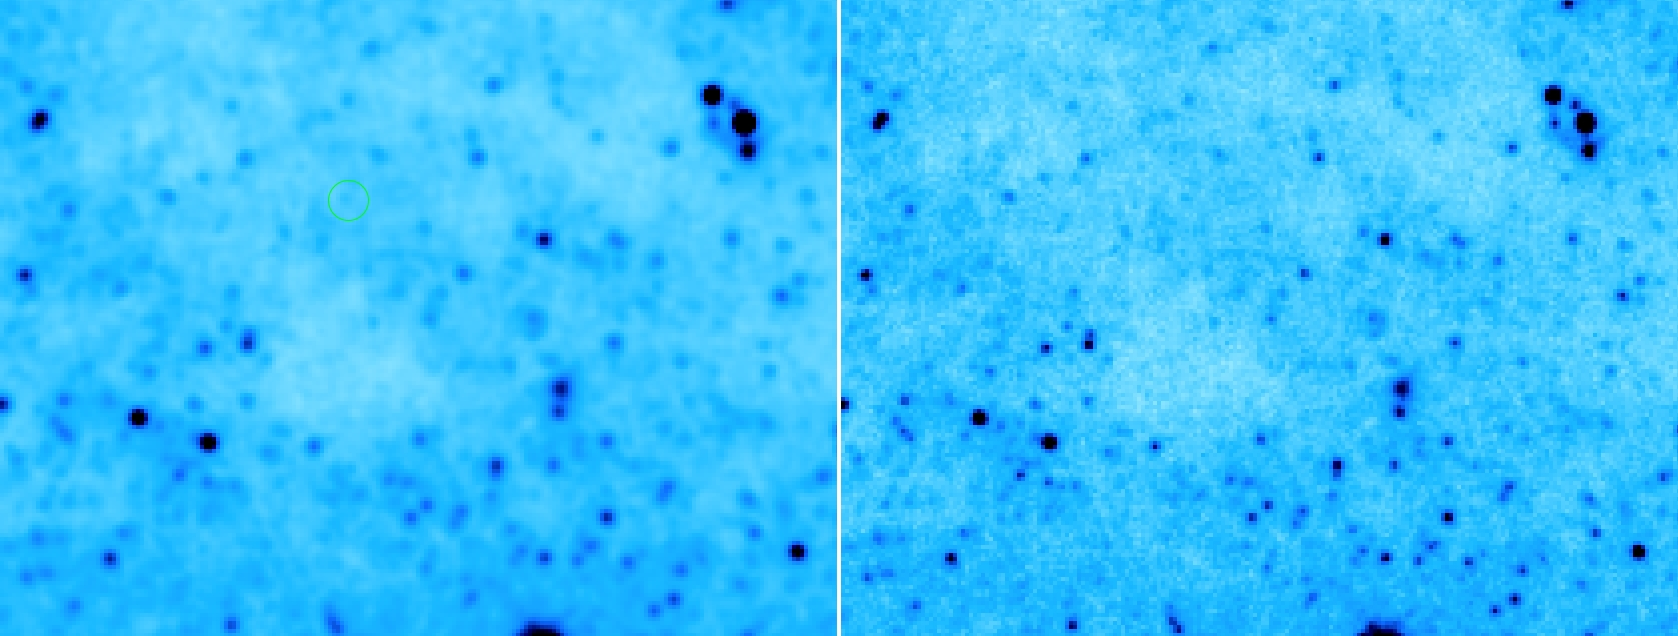
\includegraphics[width=0.87\textwidth]{conv.jpg}
    \caption{In this image you can observe how an observation looks, before and after convolution, this partícular image corresponds to the B band filter and was convolved to a 0.083 arc sec FWHM}
    \label{img:conv}
\end{figure}

\begin{table}[h]
  \centering
    \begin{tabular}{ c c c }
    \hline\hline
    
    Filter / Config. & Central $\lambda$ & FWHM (arc sec)\\
    \hline
    
    F225W & 235.9 nm & $\sim$0.083\\
    
    F336W & 335.5 nm & $\sim$0.075\\
    
    F373N & 373.0 nm & $\sim$0.070\\
    
    F438W & 432.5 nm & $\sim$0.070\\
    
    F487N & 487.1 nm & $\sim$0.067\\
    
    F502N & 501.0 nm & $\sim$0.067\\
    
    F657N & 656.7 nm & $\sim$0.070\\
    
    F673N & 676.6 nm & $\sim$0.070\\
    
    F814W & 802.4 nm & $\sim$0.074\\
    
    \hline
  \end{tabular}
  \caption{WFC3/UVIS PSF FWHM informations for the selected dataset, as you can see the largest number here is 0.083 which means the poorest spatial resolution, this is the number used to calculate the convolution kernel, in order to precess them all images must have the same spatial resolution.}
  \label{tab:dos}
\end{table}


\begin{figure}[h]
	\centering
    \includegraphics[width=0.47\textwidth]{uno.jpg}
    \caption{Look at the image, it is composed of two mosaics, therefore, there are some regions with missing data, now look at the borders of each mosaic there is noise near the edges, this is data that we don't want messing with our clustering algorithm and can be classified as outliers, it is very important to reduce them as much as possible so the output clusters can be correctly classified and correspond to the information that we are looking for}
    \label{img:dos}
\end{figure}



Well, what I wrote before it is a brief summary of what I did, but I'm sure that you can find a better way to do your own data pre-processing but here are some things that you should consider:
	\begin{itemize}
    	\item Create a method as general as possible, with input parameter that can be adapted to any kind of data, this will save you a lot of work in the future
        \item Understand first your algorithm, how the data is going to be processed and design the best way to input your data
        \item Accommodate your data according to the type of attributes that the algorithm can handle
        \item Consider the size of your dataset, if it's huge your program may never end
        \item Find out of your algorithm can work with high dimensional data (multi-wavelength), because if not, you won't be able to input data cubes
        \item Find out if your selected clustering algorithms is able to find clusters of irregular shapes, this will help you to device the best way to accommodate your patterns
        \item Handle outliers, if you identify them, know where they are, try to eliminate them as much as possible, we don't want them messing with our clusters
        \item In case that you come up with an artful mathematical method like PCA to reduce dimensionality, make sure that what you input can later make sense when is clustered, because you will be working in another space
        \item Remember that the most important goal is to find hidden knowledge therefore, you must know you to visualize and interpret your results
        \item For the let's call it \emph{astronomy image processing}, make sure that your data is scientifically approved ask people around you.
    \end{itemize}

This section is explained at length in the GitHub page, there you will find my codes and some helpful links, \url{https://github.com/LaurethTeX/Clustering/blob/master/Preprocessing.md}

\section{Software available}



This specific part is all explained in GitHub in this link. \url{https://github.com/LaurethTeX/Clustering/blob/master/Preprocessing.md#first-step-data-pre-processing}

\begin{remark}
	Some links to start,
    \begin{itemize}
    	\item Astropy, Convolution and filtering, \url{http://docs.astropy.org/en/stable/convolution/index.html}
        \item AstroDrizzle: New Software for Aligning and Combining
HST Images, With Improved Handling of Astrometric Data, \url{http://drizzlepac.stsci.edu/}
		\item Tiny Tim HST PSF Modelling, \url{http://www.stsci.edu/hst/observatory/focus/TinyTim}
        \item IRAF, Image Reduction and Analysis Facility, \url{http://iraf.noao.edu/}
    \end{itemize}
\end{remark}


%----------------------------------------------------------------------------------------
%	CHAPTER 4
%----------------------------------------------------------------------------------------

\chapterimage{head1.png} % Chapter heading image

\chapter{Experimenting}
 this wasn't the best way to tackle this problem I started considering only clustering on the independent images and not in the data cube due to the fact that the dimensionality was immense. So, in the end my selected methods have some results but not all, here is where all the work has to be done, analysed and tested again.

\section{Methods Selected}

\subsection{ESOM, Evolving Self Organizing Maps}
The \emph{official} manual for this method can de found here, \url{http://dame.dsf.unina.it/documents/ESOM_UserManual_DAME-MAN-NA-0021-Rel1.2.pdf}, there you will find a full explanation of the method, the meaning of 

The method is divided in three stages, \emph{Train}, \emph{Test} and \emph{Run}.
The first step to experiment with this method is Train. Here, the important variables to understand an look at are, the learning rate, epsilon and the pruning frequency. It is highly recommendable that you check the DAMEWARE manual for this function, there they will explain in detail the meaning of each on the mentioned variables.

\subsubsection{Expected Results}
	This partícular method as I mentioned before supports data cubes and considers as an independent pattern all the  numbers in the multi-dimensional array this means that our clusters are groups of patterns with similar characteristics, that correspond to volumes of similar fluxes of electrons inside the data cube.
    
    The output files from the experiment that will show us our results are, 
    \begin{itemize}
    	\item \emph{E\_SOM\_Train\/Test\/Run\_Results.txt}: File that, for each pattern, 
reports ID, features, BMU, cluster and activation of winner node
		\item \emph{E\_SOM\_Train\/Test\/Run\_Histogram.png}: Histogram of clusters found 
        \item \emph{E\_SOM\_Train\/Test\/Run\_U\_matrix.png}: U-Matrix image 
        \item \emph{E\_SOM\_Train\/Test\/Run\_Clusters.txt}: File that, for each clusters, reports label, number of pattern assigned, percentage of association respect total number of pattern and its centroids. 
        \item \emph{E\_SOM\_Train\_Datacube\_image.zip}: Archive that includes the 
clustered images of each slice of a data cube.\footnote{I have my doubts whether this file is produced or not, in none of my test was produced, you might need to contact the developers and ask about this.}
    \end{itemize}
The file that you will be looking forward to see is the last one, the zip where you will be able to see the slices of the volume, and how the final configuration of the clusters was arranged.

\subsubsection{Failed and still running tests: What no to do and what is still running}
 

In table \ref{tab:ds9failed} are the input parameters I used to the failed tests applied in the \emph{raw} data cube, and in table \ref{tab:ds9running} are the input parameters used on experiments that are still running since August 7th, 2014. (I wonder if they will ever end)

\begin{table}[h!]
  \centering
    \begin{tabular}{ c c c c c c }
    \hline\hline
    
    Name & Input nodes & Normalized data & Learning rate & Epsilon & Pruning Frequency\\
    \hline
    
    Train2 & 1 & 1 & 0.3 & 0.001 & 5\\
    Train3 & 1 & 1 & 0.7 & 10 & 100\\
    Train4 & 1 & 1 & 0.95 & 1 & 10\\
    Train5 & 1 & 1 & 0.99 & 0.1 & 10\\
    Train6 & 1 & 1 & 0.01 & 0.01 & 1\\
    Train7 & 1 & 1 & 0.5 & 0.7 & 5\\
    Train8 & 1 & 1 & 0.5 & 0.5 & 7\\
    Train11 & 1 & 1 & 0.25 & 0.00001 & 10\\
    
    \hline
  \end{tabular}
  \caption{This table describes all the failed experiments done in the workspace WFC3 with the \emph{raw} data cube as an input, using the ESOM method in the DAME platform selecting the number 3 as the dataset type and without using a previous configuration file.}
  \label{tab:ds9failed}
\end{table}

\begin{table}[h!]
  \centering
    \begin{tabular}{ c c c c c c }
    \hline\hline
    
    Name & Input nodes & Normalized data & Learning rate & Epsilon & Pruning Frequency\\
    \hline
    
    Train9 & 1 & 1 & 0.3 & 0.0001 & 5\\
    Train10 & 1 & 1 & 0.99 & 0.0001 & 10\\
    Train12 & 1 & 1 & 0.5 & 0.0001 & 5\\
    
    \hline
  \end{tabular}
  \caption{This table describes all the experiments done in the workspace WFC3 that are still running since August 7th, 2014 with the \emph{raw} data cube as an input, using the ESOM method in the DAME platform selecting the number 3 as the dataset type and without using a previous configuration file.}
  \label{tab:ds9running}
\end{table}

Some of the failed experiments had histogram like the one you can see on figure \ref{img:faildtrain2} where the clusters were created but reached a point where the neural network could not define how to differentiate a cluster from another cluster and failed.

\begin{figure}[h!]
	\centering
    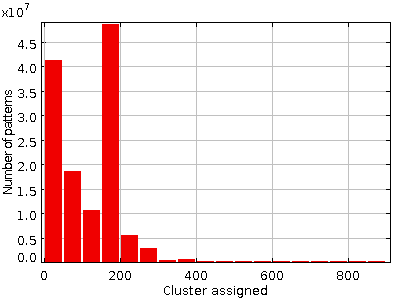
\includegraphics[width=0.47\textwidth]{Histogram_train2.png}
    \caption{In this partícular experiment, the neural network failed due to a very low pruning frequency, high number of patterns and all the outliers inclusions.}
    \label{img:faildtrain2}
\end{figure}




\begin{table}[h!]
  \centering
    \begin{tabular}{ c c c c c c }
    \hline\hline
    
    Name & Input nodes & Normalized data & Learning rate & Epsilon & Pruning Frequency\\
    \hline
    
    TrainHa1 & 1 & 1 & 0.5 & 0.01 & 5\\
    TrainHa2 & 1 & 1 & 0.5 & 0.001 & 5\\
    
    \hline
  \end{tabular}
  \caption{This table describes the failed experiments done in the workspace WFC3 for the \emph{halpha\_conv.fits} file, using the ESOM method for one layer in the DAME platform selecting the number 3 as the dataset type and without using a previous configuration file.}
  \label{tab:hafailed}
\end{table}

\begin{table}[h!]
  \centering
    \begin{tabular}{ c c c c c c }
    \hline\hline
    
    Name & Input nodes & Normalized data & Learning rate & Epsilon & Pruning Frequency\\
    \hline
    
    TrainHa3 & 1 & 1 & 0.5 & 0.0001 & 5\\
    
    \hline
  \end{tabular}
  \caption{This table describes the still running experiments since August 10th, 2014 in the workspace WFC3 for the \emph{halpha\_conv.fits} file, using the ESOM method for one layer in the DAME platform selecting the number 3 as the dataset type and without using a previous configuration file.}
  \label{tab:harun}
\end{table}



\begin{table}[h!]
  \centering
    \begin{tabular}{ c c c c c c }
    \hline\hline
    
    Name & Input nodes & Normalized data & Learning rate & Epsilon & Pruning Frequency\\
    \hline
    
    Train1 & 1 & 1 & 0.5 & 0.001 & 50\\
    Train2 & 1 & 1 & 0.5 & 0.01 & 50\\
    Train3 & 1 & 1 & 0.5 & 0.1 & 100\\
    Train4 & 1 & 1 & 0.5 & 0.001 & 100\\
    
    \hline
  \end{tabular}
  \caption{This parameters where used in three different workspaces (\emph{halphaCrop, uvwidecrop, ibandcrop}), with their own input file that corresponded to the convolved and cropped observation of each filter (halpha\_conv\_crp.fits, uvwide\_conv\_crp.fits, iband\_conv\_crp.fits), all of the experiments had no previous configuration file and the dataset type was 3 and all failed.}
  \label{tab:threefail}
\end{table}

\begin{figure}[h!]
	\centering
    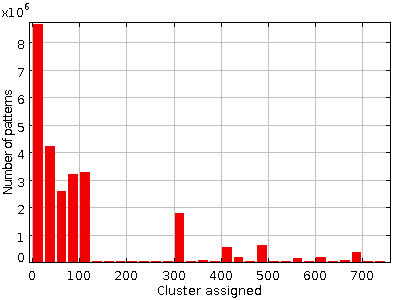
\includegraphics[width=0.31\textwidth]{Histogram-halpha1.png}
    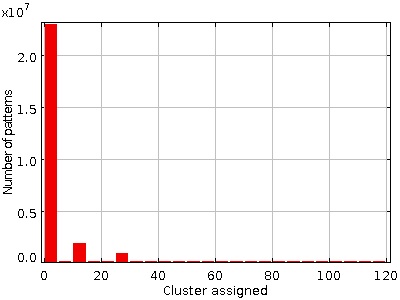
\includegraphics[width=0.31\textwidth]{Histogram-uvwide-2.png}
    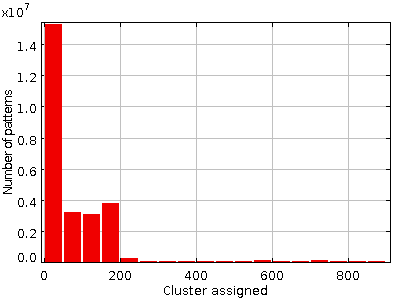
\includegraphics[width=0.31\textwidth]{Histogram-iband3.png}
    \caption{The histogram on the left corresponds to the halpha workspace in Train1, the one on the center to the iband workspace in Train3 and the one on the right to the uvwide workspace in Train2, all of them were failed experiments.}
    \label{img:fail3}
\end{figure}

\begin{table}[h!]
  \centering
    \begin{tabular}{ c c c c c c }
    \hline\hline
    
    Name & Input nodes & Normalized data & Learning rate & Epsilon & Pruning Frequency\\
    \hline
    
    Train5 & 1 & 1 & 0.5 & 0.0001 & 100\\
    Train6 & 1 & 1 & 0.99 & 0.0001 & 75\\

    \hline
  \end{tabular}
  \caption{This parameters where used in three different workspaces (\emph{halphaCrop, uvwidecrop, ibandcrop}), with their own input file that corresponded to the convolved and cropped observation of each filter (halpha\_conv\_crp.fits, uvwide\_conv\_crp.fits, iband\_conv\_crp.fits), all of the experiments had no previous configuration file and the dataset type was 3. The experiments mentioned are still running since August 11th, 2014.}
  \label{tab:threerun}
\end{table}

As you can see, I discovered that if I choose an epsilon of 0.0001 the experiments will be still running, and all of the other variables can be variated like the learning rate and the pruning frequency.

\subsubsection{The big and small re-projected data cube}
After a few days of waiting anxiously for the experiments to end and not getting any new results I decided to test the convolved, cropped and re-projected data cube including all the layers with a fixated pruning frequency of 0.0001, hopping that this time I could get some interesting results. The input parameters for the two experiments I tested can be seen in table \ref{tab:cubeesom}.

\begin{table}[h!]
  \centering
    \begin{tabular}{ c c c c c c }
    \hline\hline
    
    Name & Input nodes & Normalized data & Learning rate & Epsilon & Pruning Frequency\\
    \hline
    
    ESOMtrain1 & 1 & 1 & 0.5/0.75 & 0.0001 & 100\\
    ESOMtrain2 & 9 & 1 & 0.75 & 0.001 & 100\\

    \hline
  \end{tabular}
  \caption{This parameters where used in two different workspaces (\emph{Data Cube, RPDataCube}), the first experiment is still running since August 12th, 2014 and the second fail}
  \label{tab:cubeesom}
\end{table}


 I selected randomly a partícular HII region located in RA 204.26971, DEC -29.84933 (See figure \ref{img:h2region}) and centred it in a 605x605 pixels sample.

\begin{figure}[h!]
	\centering
    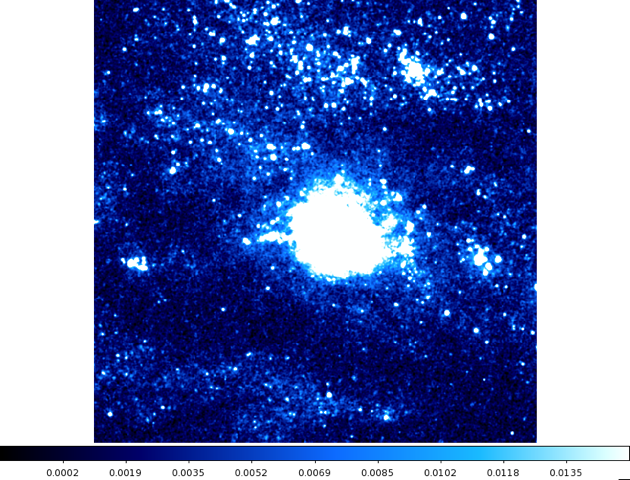
\includegraphics[width=0.52\textwidth]{small_ex.png}
    \caption{Illustration of the randomly chosen HII region for the small sample from the M83 re-projected data cube.}
    \label{img:h2region}
\end{figure}

This time, most of the experiments gave me immediate results failing or finishing. On table \ref{tab:small}, you can see the input parameters and the status of the experiments I tested with the small data cube.

\begin{table}[h!]
  \centering
    \begin{tabular}{ c c c c c c }
    \hline\hline
    
    Name & Normalized & Learning rate & Epsilon & Pruning Frequency & Status\\
    \hline
    
    ESOMtrain1 & 0 & 0.5 & 0.001 & 50 & Running\\
    Train2 & 1 & 0.5 & 0.0001 & 50 & Ended\\
    Train3 & 1 & 0.5 & 0.1 & 50 & Ended\\
    Train4 & 0 & 0.5 & 0.0001 & 50 & Running\\
    Train5 & 0 & 0.95 & 0.0001 & 100 & Running\\
    Train6 & 1 & 0.99 & 0.001 & 50 & Ended\\

    \hline
  \end{tabular}
  \caption{All the mentioned experiment belong to the SmallDataCube workspace, have 3 as data type and one input node, no previous configuration file and the input file is \emph{rp\_small\_datacube.fits}.}
  \label{tab:small}
\end{table}
interesting results, in the next figures (\ref{img:smallended},\ref{img:matrixended}) you can appreciate better what I'm taking about.

\begin{figure}[h!]
	\centering
    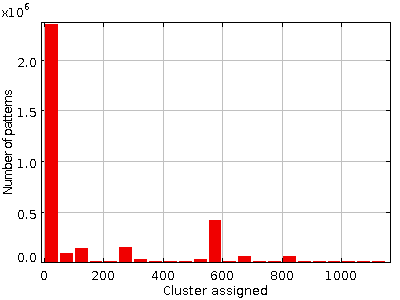
\includegraphics[width=0.31\textwidth]{Small-train2.png}
    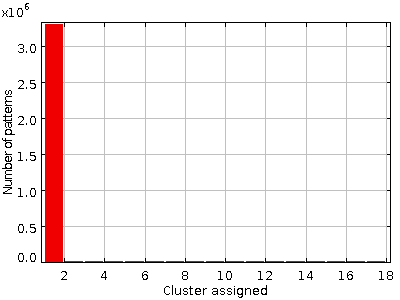
\includegraphics[width=0.31\textwidth]{Small-train3.png}
    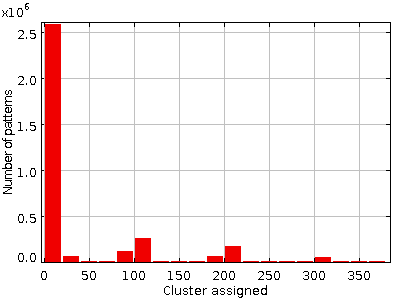
\includegraphics[width=0.31\textwidth]{Small-train6.png}
    \caption{rted, to understand further the results a visualization of the clusters is needed.}
    \label{img:smallended}
\end{figure}

\begin{figure}[h!]
	\centering
    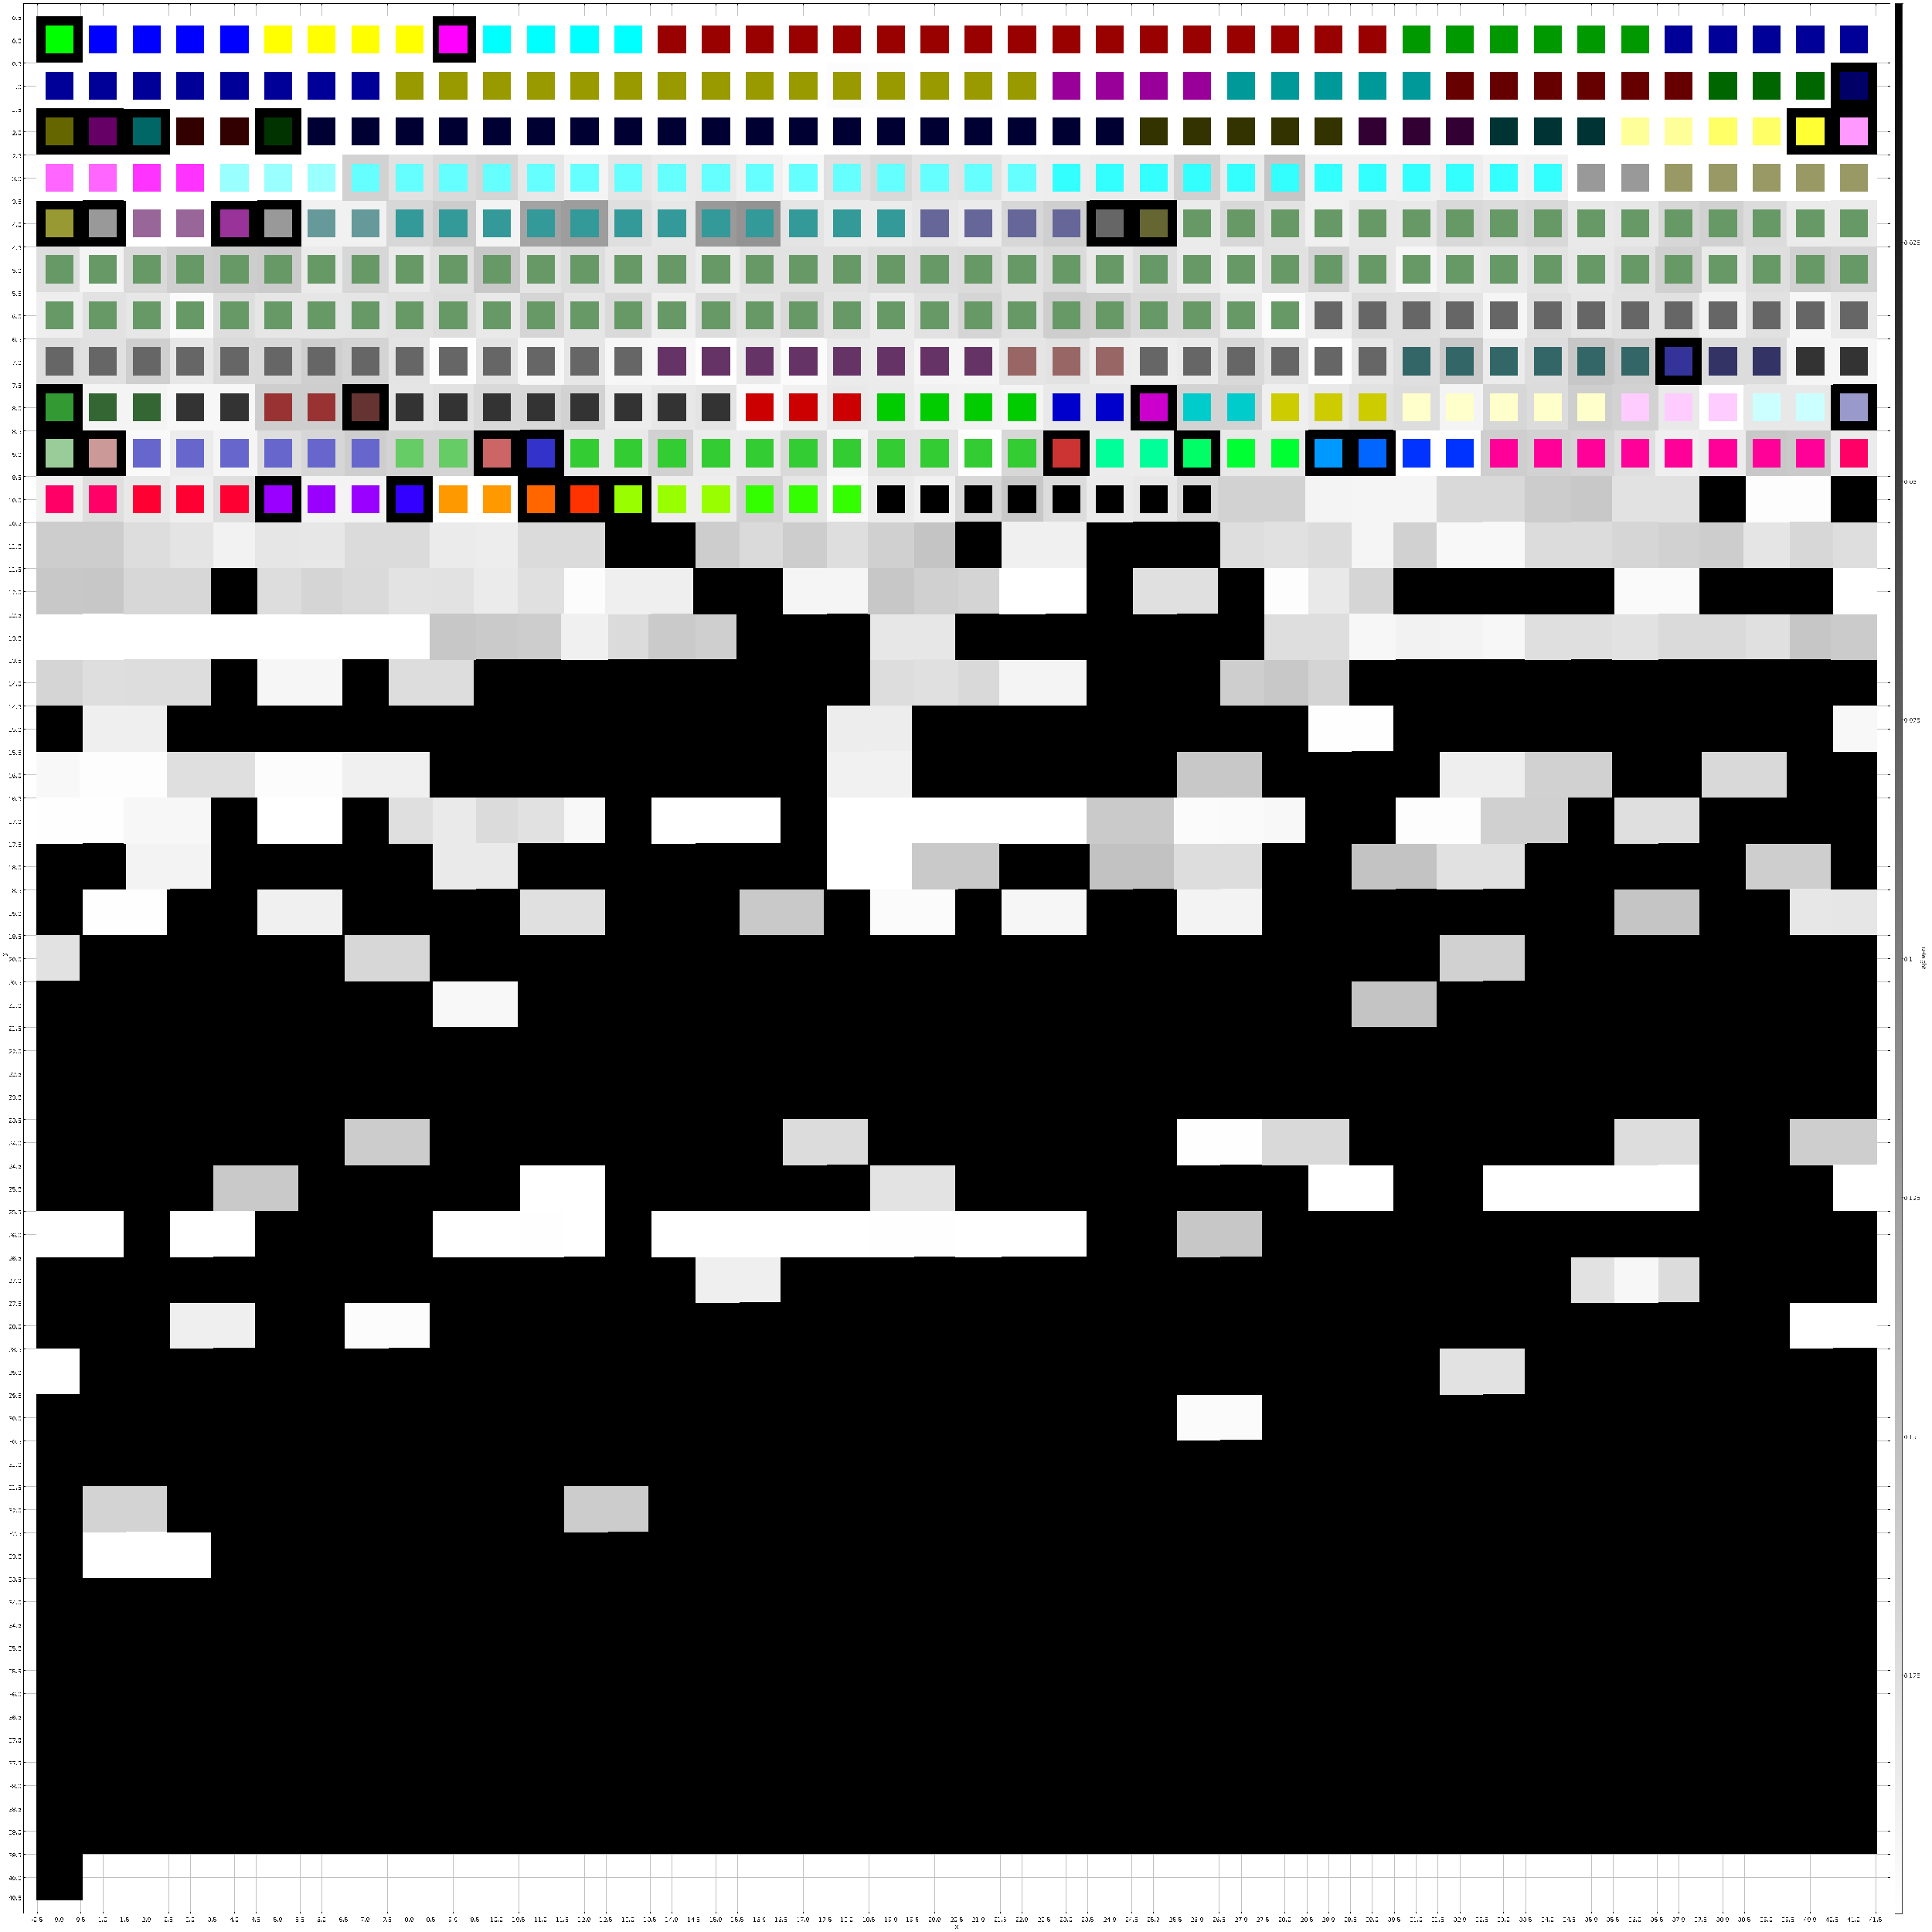
\includegraphics[width=0.31\textwidth]{matrix2-01.png}
    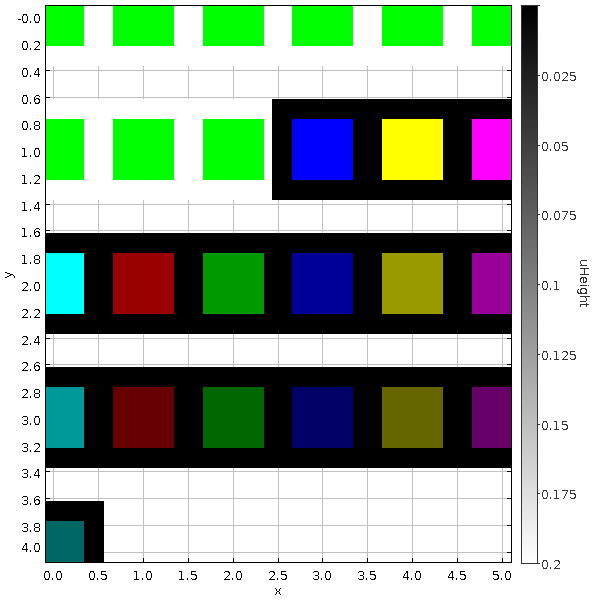
\includegraphics[width=0.31\textwidth]{Small-train3-matrix.png}
    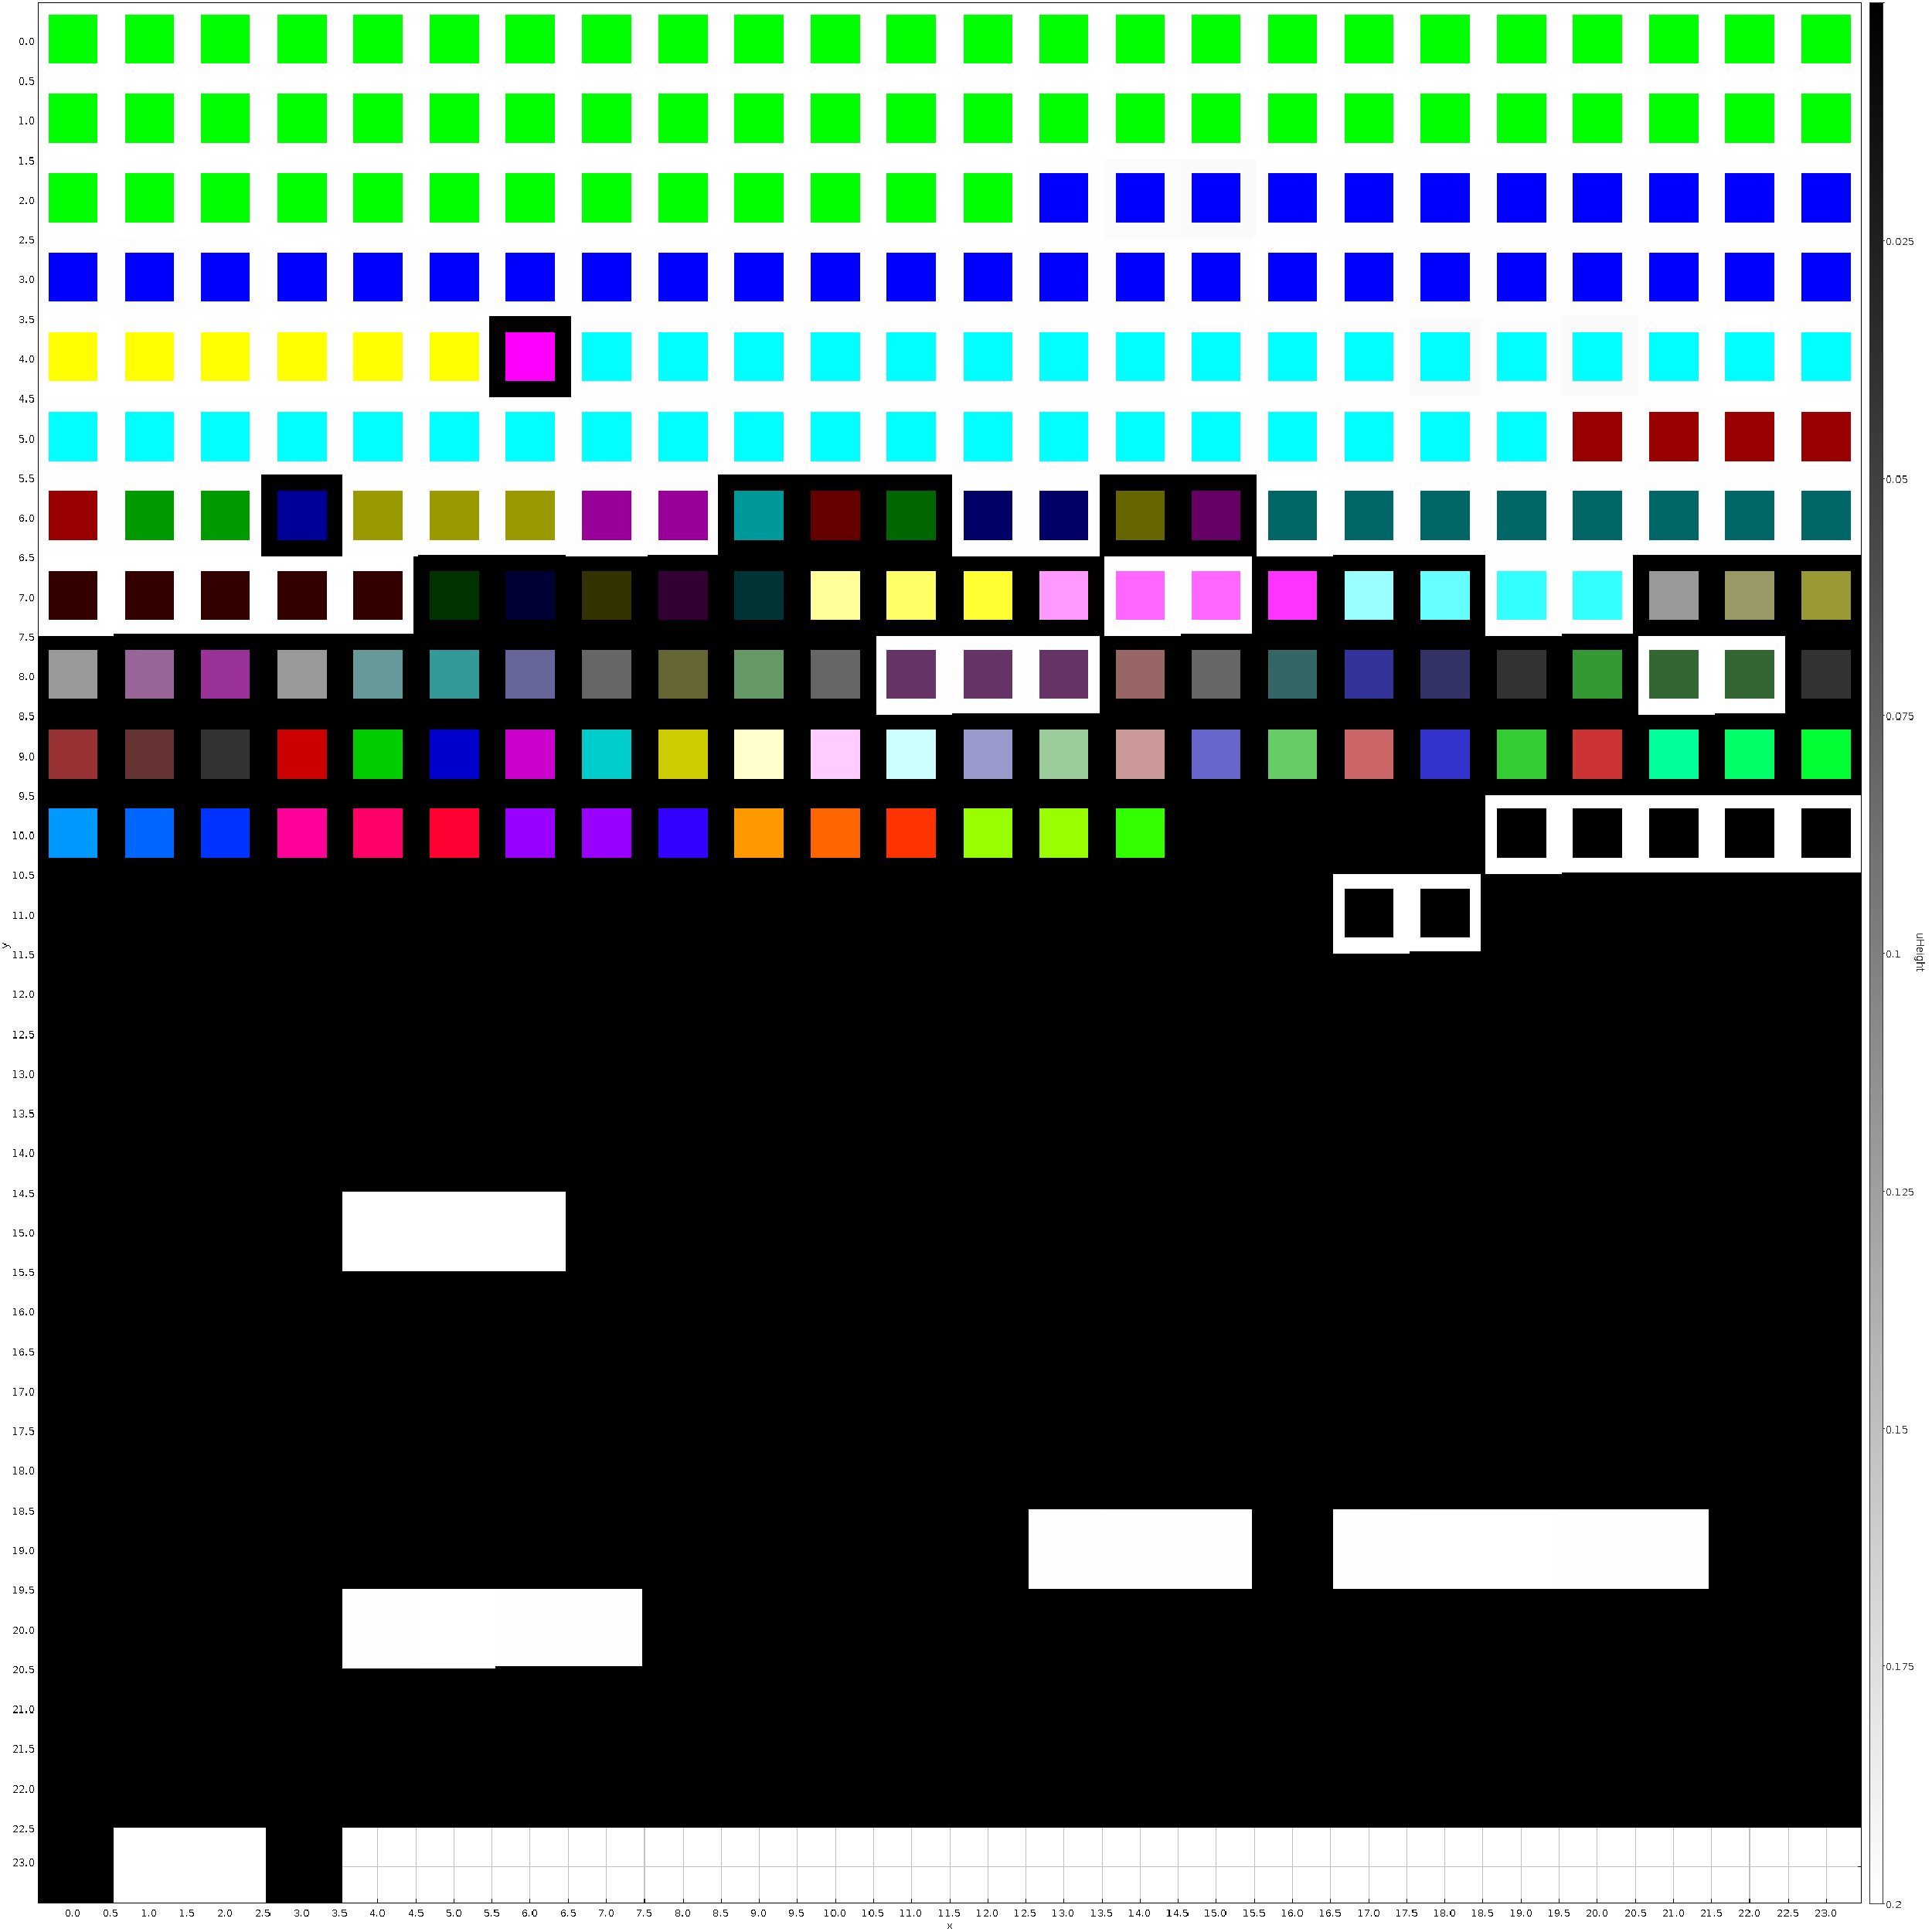
\includegraphics[width=0.31\textwidth]{matri6-01.png}
    \caption{All of the images correspond to U-matrices of the ended experiments mentioned above in order (Train2, Train3, Train6)}
    \label{img:matrixended}
\end{figure}
 There 
\subsection{CSOM}
%one image
\end{comment}

\nocite{*}
\bibliographystyle{ieeetr}
\bibliography{ref-statistics}


\vfill
\textit{Wish you all the best, Andrea Hidalgo}
\end{document}